%                                     MMMMMMMMM        
%                                                                             
%  MMO    MM   MMMMMM  MMMMMMM   MM    MMMMMMMM   MMD   MM  MMMMMMM MMMMMMM   
%  MMM   MMM   MM        MM     ?MMM              MMM$  MM  MM         MM     
%  MMMM 7MMM   MM        MM     MM8M    MMMMMMM   MMMMD MM  MM         MM     
%  MM MMMMMM   MMMMMM    MM    MM  MM             MM MMDMM  MMMMMM     MM     
%  MM  MM MM   MM        MM    MMMMMM             MM  MMMM  MM         MM     
%  MM     MM   MMMMMM    MM   MM    MM            MM   MMM  MMMMMMM    MM
%
%
%            - META-NET Language White Paper | Basque content -
% 
% ----------------------------------------------------------------------------

\begin{document}

\maketitle

\null
\pagestyle{empty} 

\makefundingnotice

\pagenumbering{Roman} 
\setcounter{page}{5}
\pagestyle{scrheadings}

\cleardoublepage

% --------------------------------------------------------------------------
\bsection*{Hitzaurrea --- Preface}

\begin{Parallel}[c]{78mm}{78mm}
\ParallelLText{\selectlanguage{basque}
Liburu zuri hau hizkuntza-teknologiei eta haien potentzialei buruzko jakintza sustatzea helburu duen bildumaren atal bat da, eta hezitzaileei, kazetariei, politikariei, hizkuntza-komunitateei eta besteri zuzenduta dago.

Europan, desberdina da, hizkuntza batetik bestera, hizkuntza-teknologien eskuragarritasuna eta erabilera. Horren ondorioz, desberdinak behar dute izan, halaber, hizkuntza bakoitzerako hizkuntza-teknologien ikerketa eta garapena bultzatzeko behar diren ekimenak. Ekimen horiek hainbat faktoreren araberakoak dira; besteak beste, hizkuntza jakin baten konplexutasuna eta haren hiztun-komunitatearen tamaina.

Europako Batzordeak sortutako META-NET Bikaintasun Sareak gaur egungo hizkuntza-baliabideei eta -teknologiei buruzko analisi bat bideratu du. Analisi hori Europako 23 hizkuntza ofizialentzako eta Europako beste zenbait nazio- eta eskualde-hizkuntza garrantzitsurentzako gauzatu da, eta, analisiaren ondorio gisa, ondorioztatu da ikerketa-hutsune esanguratsuak daudela hizkuntza bakoitzerako. Adituen gaur egungo egoeraren analisi eta ebaluazio xeheago batez, etorkizuneko ikerketen eragina handiagotu eta arriskuak gutxiagotu litezke.

Enpresa-munduko, administrazio publikoko, industria-sektoreko, ikerketa-alorreko, software-enpresetako, teknologia-hornitzaileetako eta unibertsitate europarretako parte-hartzaileekin lanean diharduten 33 herrialdetako 54 ikerketa-zentroz (p.~\pageref{metanetmembers}) osatuta dago META-NET. Denak elkarrekin, teknologiari buruzko ikuspegi bateratu bat ari dira sortzen, eta, aldi berean, 2020 bitartean ikerketa-hutsuneak hizkuntza-teknologien bidez betetzeko bideak zein izan daitezkeen azaltzen duen ikerketa-agenda estrategiko bat ere ari da garatzen.}

\ParallelRText{\selectlanguage{english}
This white paper is part of a series that promotes knowledge about language technology and its potential. It addresses educators, journalists, politicians, language communities and others. 

The availability and use of language technology in Europe varies between languages. Consequently, the actions that are required to further support research and development of language technologies also differ for each language. The required actions depend on many factors, such as the complexity of a given language and the size of its community.

META-NET, a Network of Excellence funded by the European Commission, has conducted an  analysis of current language resources and technologies in this white paper series (p.~\pageref{whitepaperseries}). This analysis focussed on the 23 official European languages as well as other important national and regional languages in Europe. The results of this analysis suggest that there are many significant research gaps for each language. A more detailed expert analysis and assessment of the current situation will help maximise the impact of additional research and minimise any risks.

META-NET consists of 54 research centres from 33 countries (p.~\pageref{metanetmembers}) that are working with stakeholders from commercial businesses, government agencies, industry, research organisations, software companies, technology providers and European universities. Together, they are creating a common technology vision while developing a strategic research agenda that shows how language technology applications can address any research gaps by 2020.} 
\ParallelPar
\end{Parallel}

\cleardoublepage

% --------------------------------------------------------------------------
\bsection*{Aurkibidea --- Table of Contents}

\renewcommand\contentsname{}

\tableofcontents
\addtocontents{toc}{\protect\thispagestyle{empty}\protect}
\addtocontents{toc}{{\Large\textsf{\centerline{EUSKARA ARO DIGITALEAN}}\par}}

\cleardoublepage


% --------------------------------------------------------------------------
\setcounter{page}{1}
\pagenumbering{arabic} 
\pagestyle{scrheadings}


% Start of origin language part
% --------------------------------------------------------------------------
\ssection[Laburpena]{Laburpena}

\selectlanguage{basque}

\begin{multicols}{2}
Hizkuntza gizakien arteko komunikazio-biderik garrantzitsuena da. Ideiak eta sentimenduak adierazteko aukera ematen digu, ikasten eta irakasten laguntzen digu, ezinbestekoa da bizitzeko, kulturaren transmisiorako tresnarik garrantzitsuena da, eta haren hiztunen identitate-ikurra da.

   \boxtext{Hizkuntza gizakien arteko komunikazio-biderik garrantzitsuena da}

Gaur egun, mundu globalizatu honetan, edozein lekutako pertsonekin erraz komunikatzeko tresna asko ditugu. Adibidez, informazio- eta komunikazio-teknologia berriek sare sozialak garatzeko aukera eman dute, eta, hala, ekarpen handia izan da herrialde eta kultura desberdinetako pertsonak harremanetan jartzea sustatzeko. Azken urteotan, halaber, atzerritarren mugimendua handia izan da gure herrialdeetan, dela turismoagatik, dela immigrazioagatik, eta horrek hainbat hizkuntzatan komunikatzeko beharra sortu du. Halere, hizkuntzarteko komunikazio-arazoak, maiz, lingua franca erabiliz gainditzen dira.

Europa aniztasun kultural eta linguistikoaren adibide garbia da, nahiz eta azken 60 urteetan zehar bateratzen politiko eta ekonomikoa izan duen. Hortaz, euskaratik polonierara zein italieratik islandierara, eragozpen linguistikoak gainditu behar dira, nahitaez, Europako hiritarren arteko eguneroko komunikazioan nahiz enpresaren eta politikaren esferetako komunikazioetan. Europar Batasunaren erakundeek bilioi bat euro behar dute urtean, beren eleaniztasun-politika betearazteko; alegia, testuak itzultzeko eta ahozko jarduerak interpretatzeko. Bitartean, ingelesa lingua franca bihurtzen ari da Europako hiritarren arteko komunikazioan.

Espainiar estatuan ere antzeko eszenatokia dugu. Estatu osoan, hizkuntza ofizial bakarra dago: espaniera edo gaztelania; horiez gainera, hiru hizkuntza koofizial daude: euskara, galiziera eta katalana. Estatuan eleaniztasunari eustea ez da lan erraza izan; aitzitik, espainierak gainerako hizkuntzen artean duen gailentasunean, identitate kulturalaren eta linguistikoaren babesean oinarritutako prozesu konplexu baten emaitza izan da. Europako kasuan lingua franca gisa ingelesa erabiltzen den era berean, espainiera erabiltzen da maiz espainiar estatuko hizkuntza-eremu desberdinetako hiritarren arteko komunikazio zuzenerako.   

 \boxtext{Eleaniztasuna babestu beharreko kultura-ondarea da}
 
Bai Europari dagokionez, bai espainiar estatuari dagokionez, babestu beharreko kultura-ondarea da eleaniztasuna. Globalizazioak, lingua francaren erabilera gailendu eta gure hizkuntzaren erabilera murrizteko arriskua sortzen baitu, ez luke gure hizkuntza- eta kultura-ondare aberatsa alboratzen duen mekanismo bihurtu behar. Komunikazio-mundu global baten barnean, gure hizkuntza eta, harekin batera, gure identitate kulturala babesteko bideak aurkitu behar ditugu.

Gaur egungo hizkuntza-teknologiek eta ikerketa linguistikoek ekarpen handia egin dezakete eragozpen linguistiko horiek gainditzeko; izan ere, hizkuntza-teknologiak, tresna eta aplikazio adimendunekin batera erabiliz, oso lagungarriak izango dira europarrek aise hitz egin eta salerosketak egin ditzaten, baita hizkuntza berean ari ez badira ere. Hizkuntza-teknologiek eskaintzen dituzten koponbideak hizkuntza europarren arteko zubi bikaina izan daitezke. Gaur egun merkatuan lor daitezkeen itzulpen automatikoko nahiz hizketa prozesatzeko tresnak –galderei erantzuteko sistemetatik hasi eta hizkuntza naturala darabilten interfazeetaraino, eta, besteak beste, itzulpen automatikoko sistemak eta laburpen-tresnak darabiltenak–, oraindik ere aski urrun daude asmo handiko helburu horretatik.

\boxtext{Hizkuntza-teknologiek eskaintzen dituzten koponbideak hizkuntza europarren arteko zubi bikaina izan daitezke}

1970eko hamarkadaren amaierarako, EB konturatua zen hizkuntza-teknologiek Europaren batasunaren gidaritzan izango zuten garrantziaz, eta, hala, lehen ikerketa-proiektua sortu zuen. Aldi berean, oso emaitza baliagarriak izan zituzten estatu-mailako proiektu asko ere jarri zituzten abian, baina inoiz ere ez europar ekintza kontzertatu baten gidaritzapean. Eremuko eragilerik garrantzitsuenak, batez ere, egoitza Amerikako Estatu Batuetan duten enpresa pribatu irabazi asmodunak dira. Gaur egungo hizkuntz-teknologia aurreratuenak hurbilketa estatistiko ez-zehatzetan oinarritzen dira eta ez dute aparteko metodo nahiz ezagutza linguistikorik erabiltzen. Esaterako, esaldiak automatikoki itzultzen dira esaldi bat gizakiek aurrez itzulitako milaka esaldirekin konparatuz. Emaitzaren kalitatea, hein handi batean, erabiliko den corpusaren tamainaren eta kalitatearen araberakoa da. Azaleko metodo estatistiko horiekin testu-material kantitate nahikoa duten hizkuntzetan esaldi sinpleak itzulita emaitza erabilgarriak lor daitezke, baina litekeena da huts egitea hizkuntza baten testu kopurua txikiagoa baldin bada edo egitura konplexuak dituzten esaldiak itzuli nahi badira. Hizkuntzen egitura-ezaugarri sakonagoa aztertuta, ondoriozta daiteke aurrerabide bakarra dela, Europako hizkuntza multzo zabaleko guztietarako ondo funtzionatuko duten aplikazioak garatuko badira.

Hortaz, hizkuntzarteko komunikazio-arazoen konponbidea da teknologia giltzarriak garatzea. Helburu hori betetzeko, baina Europako kultura- eta hizkuntza-aniztasunari eutsita, behar-beharrezkoa da lehendabizi Europako hizkuntza guztien bereizgarri linguistikoak aztertzea eta hizkuntza bakoitzerako hizkuntza-teknologiek duten gaur egungo laguntzen analisi sistematiko bat burutzea. Euskararako analisia aurkeztea da, hain zuzen, liburu honen xedea. Hala, euskarako hizkuntza-teknologien, aplikazioen eta konponbideen analisi xehatua aurkezten du ale honek.

\boxtext{Euskara ikerketa sustatu beharra duten EBko hizkuntzetariko bat da}

Hizkuntza-teknologien eremuan, hainbat produktu, teknologia eta baliabide daude euskararako. Badira aplikazio-tresnak hizketa sintetizatzeko, hizketa ezagutzeko nahiz ortografia zuzentzeko; badira, halaber, itzulpen automatikoko aplikazio batzuk ere, espainieratik euskarara batez ere. 

Liburu zuri bilduma honetan ageri denez, ikaragarrizko aldea dago Europako estatu kideen hizkuntza-baliabideen inbentarioen artean eta ikerketa-egoeren artean. Ondoriorik nabarmenenetariko bat da ikerketa sustatu beharra duten EBko hizkuntzetariko bat dela euskara, hizkuntza-teknologietan oinarritutako aplikazio benetan eraginkorrak eta egunero jardunean erabiltzeko modukoak garatuko badira. Euskararako kalitate handiko hizkuntza teknologiaren garapena oso larria eta garrantzitsua da euskara sustatzeko.

\end{multicols}

\clearpage


% --------------------------------------------------------------------------
\ssection[Arriskua, gure hizkuntzentzat, eta erronka, hizkuntza-teknologiarentzat]{Arriskua, gure hizkuntzentzat \newline  eta erronka\newline hizkuntza-teknologiarentzat}

\begin{multicols}{2}
    Komunikazioan eta gizartean izugarrizko eragina izaten ari den iraultza digital baten aurrean gaude. Komunikazio-teknologia digitalizatu eta sarekoetan izan berri diren aurrerapenak Gutenbergek inprenta asmatu zuenekoarekin alderatzen dira, batzuetan. Zer esaten digu analogia horrek Europako informazio-gizartearen eta geure hizkuntzen etorkizunari buruz?
\boxtext{Iraultza digitala Gutenbergek inprenta asmatu izanarekin alderatu daiteke}

Gutenbergen asmakizunaren ondoren, benetako aurrerapausoak eman ziren komunikazioan eta ezagutzen trukaketan, hainbat lani esker; esaterako, Lutherrek eginikoa, Biblia hizkuntza arrunt batera itzuli zuenean. Hurrengo mendeetan, teknika kulturalak garatu dira hizkuntza-prozesamendua eta ezagutza- trukaketa hobeto egiteko:
 
\begin{itemize}
      \item Hizkuntza handien ortografia eta gramatika estandarizatzeak aukera eman zuen ideia zientifiko eta intelektual berriak azkar zabaltzeko;
      \item Hizkuntzen ofizialtasunak aukera eman zien herritarrei muga jakin batzuen barruan (sarritan, politikoak) komunikatzeko;
      \item Hizkuntzen irakaskuntzari eta itzulpenari esker, hizkuntzen arteko trukaketa etorri zen;
      \item Kazetaritzako eta bibliografiako jarraibideak sortzeak material argitaratuaren kalitatea eta eskuragarritasuna bermatu zuten;
      \item Hedabide berriek —egunkariek, irratiak, telebistak, liburuek eta beste batzuek— komunikazio-beharrei erantzun zietent.
\end{itemize}
Azken hogei urteotan, informazio-teknologiak lagundu egin du prozesu horietako asko automatizatzen eta errazten:
\begin{itemize}
      \item Autoedizioko softwareak hartu du idazmakinaren eta monotipoaren tokia;
      \item Microsoft PowerPoint programak hartu du proiektagailuz erakutsitako gardenkien tokia;
      \item Mezu elektronikoen bidez faxez baino azkarrago bidali eta jasotzen dira dokumentuak;
      \item Skype erabiliz, Interneteko telefono-deiak egin daitezke, eta elkargune birtualak sortu;
      \item Audio- eta bideo-fitxategien kodetze-formatuei esker, erraza da multimedia-fitxategiak trukatzea;
      \item Bilatzaileetan gako-hitzak sartuz web-orrietara sar gaitezke;
      \item Lineako zerbitzuek itzulpen azkar eta gutxi gorabeherakoak sortzen dituzte; hor dugu, esaterako, Google Translate;
      \item Gizarte-hedabideen plataformek erraztu egiten dute elkarlana eta informazioa partekatzea. 
\end{itemize}
   Tresna eta aplikazio horiek lagungarriak badira ere, oraindik ez dute lortu informazio-gizarte europar eleaniztun eta jasangarri bat ezartzea; gizarte moderno eta inklusibo bat, non informazioa eta produktuak askatasunez ibiltzen diren alde batetik bestera.

\subsection{Hizkuntza-mugek oztopoak jartzen dizkiote Europako informazio-gizarteari}
  
Ezin dugu jakin etorkizuneko informazio-gizartea zehazki nolakoa izango den. Europaren energia-estrategiaz edo atzerriko politika bateratuaz hitz egin behar denean, Europako atzerriko ministroak beren jatorrizko hizkuntzan mintzatzen entzun nahi izango ditugu, beharbada. Agian, plataforma bat izan nahi dugu, non hainbat hizkuntza hitz egiten dituzten eta era askotako hizkuntza-mailak dituzten pertsonak gai jakin bati buruz solasean arituko diren, teknologiak haien iritziak bildu eta laburpen txikiak egiten dituen bitartean. Baliteke, halaber, beste herrialde batean dagoen osasun-aseguruen bulego batekin hitz egin nahi izatea.

\boxtext{Ekonomia- eta informazio-eremu globalak hizkuntza, hizlari eta eduki desberdinen aurrean jartzen gaitu}

Argi dago gaur egungo komunikazioak, duela urte batzuetakoaren aldean, beste kalitate batekoa izan behar duela. Ekonomia eta informazio-eremu globalean, hizkuntza, hiztun eta eduki gehiagorekin egiten dugu topo, eta hedabide mota berriekin berehala harremanetan jartzeko eskatzen digute. Gizarte-hedabideak (Wikipedia, Facebook, Twitter eta YouTube) izaten ari diren arrakasta icebergaren tontorra besterik ez da.

Gaur egun, hainbat gigabyteko testuak bidal ditzakegu mundu osora segundo gutxi batzuetan, ulertzen ez dugun hizkuntza batean dagoela ohartu baino lehen. Europako Batzordeak eskatuta duela gutxi egin den txosten baten arabera, Europako Internet-erabiltzaileen \% 57k bere jatorrizko hizkuntzaz bestelako hizkuntzetan erosten ditu produktuak eta zerbitzuak (ingelesa da gehien erabiltzen den atzerriko hizkuntza, eta, haren ondoren, frantsesa, alemana eta gaztelania). Erabiltzaileen \% 55ek irakurtzen ditu edukiak atzerriko hizkuntza batean, baina soilik \% 35ek idazten ditu mezu elektronikoak edo sareko iruzkinak \cite{BAS-Nota1}.  Duela urte gutxi batzuk, ingelesa izan zen sareko lingua franca —sareko edukiaren parte oso handi bat ingelesez zegoen—, baina egoera goitik behera aldatu da orain. Beste hizkuntza batzuetan idatzitako edukien kantitatea izugarri handitu da sarean (batez ere, asiar eta arabiar hizkuntzetan idatzitakoena).

Hizkuntza-mugek eragin duten nonahiko banaketa digitalak ez du toki handirik hartu diskurtso publikoan. Alabaina, galdera bat sortzen du behin eta berriz: “Europako zein hizkuntzak egingo du aurrera eta iraungo du sareko informazioaren eta ezagutzaren gizartean?”.

\subsection{Gure hizkuntzak arriskuan}

    Inprentak informazio-trukaketa eskerga ekarri zuen Europara, baina bertako hizkuntza asko desagertzea ere eragin zuen. Eskualdeetako hizkuntzak eta hizkuntza txikiak apenas erabiltzen ziren argitalpenetarako. Horren ondorioz, hizkuntza asko ahozko transmisiora mugatu ziren —adibidez, kornubiera eta dalmaziera—, eta, beraz, mugatuta gelditu zen haien etengabeko ikaskuntza, zabalkundea eta erabilera. 

\boxtext{Hizkuntza-aniztasuna da Europako kultura-ondasun aberats eta garrantzitsuenetarikoa}

Hizkuntza-aniztasuna da Europaren kultura-ondasun aberats eta garrantzitsuenetakoa (80 bat hizkuntza ditu). Europaren hizkuntza-aniztasuna haren arrakasta sozialaren ezinbesteko parte ere bada.  Hiztun askoko hizkuntzek eutsiko diote suspertzen ari den gizartean eta merkatu digitalean duten tokiari, dudarik gabe, baina baliteke Europako hizkuntza asko komunikazio digitaletatik baztertuta geratzea eta garrantzia galtzea Interneteko gizartearen begietara. Hori ez litzateke batere ona izango. Alde batetik, aukera estrategiko bat galduko litzateke, eta horrek ahuldu egingo luke Europaren posizioa munduan. Bestetik, gertaera horiek ez datoz bat Europako herritar guztien (edozein hizkuntza izanda ere) berdintasunezko parte-hartzea bermatzeko helburuarekin. UNESCOk eleaniztasunaren inguruan eginiko txostenak dioenez, hizkuntza funtsezko bitartekoa da oinarrizko eskubideez gozatzeko —adibidez, adierazpen politikoa, hezkuntza eta gizarteko parte hartzea— \cite{BAS-Nota3}.

\subsection{Hizkuntza-teknologia teknologia bideratzaile giltzarria da}

   Lehen, hizkuntzaren irakaskuntzara eta itzulpenetara bideratzen ziren inbertsioak. Adibidez, kalkulu batzuen arabera, itzulpen, interpretazio, software-lokalizazio eta webgune globalizazioaren merkatu europarra 8,4 mila milioi eurokoa zen 2008an, eta urtean \% 10 haztea espero zen \cite{BAS-Nota4}. Alabaina, merkatu horren ahalmena ez da nahikoa oraingo eta geroko beharrak asetzeko. 

Hizkuntza-teknologia teknologia bideratzaile giltzarria da, Europako hizkuntzak babestu eta bultzatu ditzakeena. Hizkuntza-teknologiak laguntza ematen dio jendeari elkarlanean aritzeko, negozioak egiteko, ezagutza besteekin banatzeko, eta eztabaida sozial eta politikoetan parte hartzeko, dena delako hizkuntza-mugak eta informatikako trebetasunak izanda ere. Hizkuntza-teknologiak laguntzen digu jada eguneroko lanetan, hala nola mezu elektronikoak idaztean, lineako ikerketa bat egitean edo hegaldi bat erreserbatzean. Eragiketa hauek egitean ere hizkuntza-teknologiaz baliatzen gara:

    \begin{itemize}
      \item Interneteko bilatzaile baten bidez informazioa aurkitzen dugunean.;
      \item Testu-prozesadore batean ortografia eta gramatika egiaztatzen dugunean;
      \item Lineako denda batean produktu baten gaineko gomendioak begiratzen ditugunean;
      \item Nabigazio-sistema baten ahozko jarraibideak entzuten ditugunean;
      \item Lineako zerbitzu baten bidez web-orriak itzultzen ditugunean.
    \end{itemize}
    Lan honetan agertzen diren hizkuntza-teknologiak etorkizuneko aplikazio berritzaileen oinarrizko osagaia dira. Hizkuntza-teknologia, normalean, teknologia bideratzailea izaten da, eta aplikazio-plataforma handiago baten barruan joan ohi da, nabigazio-sistema edo bilatzaile baten barruan adibidez. Liburu zuri honetan aztertzen da teknologia komunak hizkuntza bakoitzerako zenbateraino dauden prestatuta. 

\boxtext{Europak hizkuntza-teknologia sendoak eta modu onean erosteko modukoak behar ditu hango hizkuntza guztietarako}

Laster behar izango dugu Europako hizkuntza guztietarako hizkuntza-teknologia bat, eskuragarri dagoena, modu onean eros daitekeena eta software-esparru handiagoetan ondo integratuta dagoena. Erabiltzaileak ez du funtzio interaktiboak, multimediakoak eta eleaniztunak erabiltzerik hizkuntza-teknologiarik gabe.

\subsection{Hizkuntza-teknologiaren aukerak}

    Hizkuntza-teknologiak aukera eman diezaieke Europako hizkuntza guztiei itzulpen automatikoak egiteko, edukiak sortzeko, informazioa prozesatzeko eta ezagutzak kudeatzeko. Hizkuntza-teknologiak balio dezake, halaber, etxetresna elektroniko, aparailu, ibilgailu, ordenagailu eta robotentzako hizkuntzan oinarritutako interfaze intuitiboak garatzeko. Hainbat prototipo atera diren arren, aplikazio komertzial eta industrialak hasierako fasean daude oraindik. Ikerketan eta garapenean egin berri diren lorpenek benetako abagunea eman diote. Adibidez, itzulpen automatikoak (IA) zehaztasun handi samarra ematen du jada esparru jakin batzuetan, eta aplikazio esperimentalek informazio eleaniztuna eta ezagutza-kudeaketa eskaintzen dute, baita Europako hizkuntza askotan edukiak sortzeko aukera ere. 

Hizkuntza-aplikazioak, ahots bidezko erabiltzaile-interfazeak eta elkarrizketa-sistemak oso eremu espezializatuetan egon ohi dira eskuarki, eta errendimendu mugatua izan ohi dute maiz. Hizkuntza-teknologia hondamen eremuetako erreskate-lanetarako erabiltzea ari dira ikertzen orain. Arrisku handiko inguru horietan, itzulpenaren zehaztasuna hil ala biziko kontua izan daiteke. Antzekoa gertatzen da osasungintzan ere. Hizkuntzarteko ahalmenak dituzten robot inteligenteek biziak salba ditzakete. 

Hizkuntza-teknologiek sekulako merkatu-aukerak dituzte hezkuntzan eta entretenimenduen industrian; izan ere, jokoetan, joko hezigarrietan, simulazioetan eta prestakuntza-programetan integra daitezke. Hizkuntza-teknologiak zeregin garrantzitsua izan dezake beste hainbat tokitan ere; besteak beste, mugikorretako informazio zerbitzuetan, ordenagailuz lagundutako hizkuntza-ikaskuntzarako softwarean, Internet bidezko ikaskuntzako inguruneetan, autoebaluazio-tresnetan eta plagioak aurkitzeko gailuetan. Gizarte-hedabideen aplikazioek (adib. Twitter eta Facebook) duten arrakastak iradokitzen du gero eta gehiago behar direla hizkuntza-teknologia sofistikatuak, gai direnak mezuak behatzeko, eztabaidak laburbiltzeko, iritzi-joerak iradokitzeko, erantzun emozionalak detektatzeko, copyrightaren arau-hausteak identifikatzeko eta erabilera desegokien jarraipena egiteko.

\boxtext{Aniztasun linguistikoak sortzen dituen "eragozpenak" gainditzen laguntzen dute hizkuntza-teknologiek}

Hizkuntza-teknologiak aukera paregabea ematen dio Europar Batasunari, bai ekonomia aldetik, bai kultura aldetik. Eleaniztasuna arau bilakatu da Europan. Europako negozioak, erakundeak eta eskolak ere nazioartekoak eta askotarikoak dira. Herritarrek elkarrekin komunikatu nahi dute Europako Merkatu Batuan, oraindik ere hor dauden hizkuntza-mugez harago. Hizkuntza-teknologiak hor jarraitzen duten muga horiek gainditzen lagundu dezake, eta, era berean, hizkuntzaren erabilera askea eta irekia bultzatu. Gainera, Europako hizkuntzetarako hizkuntza-teknologia eleaniztun eta berritzaileak munduko beste herrialdeekin eta haietako komunitate eleaniztunekin komunikatzen lagunduko liguke. Hizkuntza-teknologiek nazioarteko ekonomia-aukera ugari ematen dituzte. 

\subsection{Hizkuntza-teknologiaren erronkak}

   Azken urteotan hizkuntza-teknologiak aurrerapen handi samarra egin badu ere, aurrerapen teknologikoa eta produktuen berrikuntza erritmo motelean doaz gaur egun. Ezin dugu hamar edo hogei urtez itxaron gure inguru eleaniztuneko komunikazioa eta produktibitatea areagotuko duten hobekuntza nabariak agertu arte.

\boxtext{Aurrerapen teknologikoa eta produktuen berrikuntza erritmo motelean doaz gaur egun}

Erabilera handiko hizkuntza-teknologiak —hala nola testu prozesadoreetako ortografia- eta gramatika-zuzentzaileak— hizkuntza bakarrean izaten dira normalean, eta hizkuntza gutxi batzuetan bakarrik egon ohi dira eskuragarri. Komunikazio eleaniztunerako aplikazioek sofistikazio-maila bat eskatzen dute.  Itzulpen automatikoa eta lineako zerbitzuak —esaterako, Google Translate edo Bing Translator— apartak dira dokumentu baten edukien gutxi gorabeherako itzulpenetarako. Baina, lineako zerbitzu eta IA aplikazio profesional horiek hainbat zailtasun izaten dituzte oso itzulpen zehatzak eta osatuak behar direnean. Okerreko itzulpen barregarri ezagunak asko dira (hor ditugu, esaterako, Bush edo Kohl izenen itzulpen literalak), eta agerian uzten dute zer-nolako erronkei egin behar dien aurre hizkuntza-teknologiak.

\boxtext{Aurrerabide teknologikoak arinago joan beharra du}

\subsection{Hizkuntzaren jabetzea gizakiengan eta makinetan}

   Ordenagailuek hizkuntza nola tratatzen duten eta hizkuntzaren jabetzea horren zaila zergatik den azaltzeko, ikus dezagun gizakiok nola jabetzen garen lehen eta bigarren hizkuntzez, eta, gero, itzulpen automatikoko sistemen funtzionamenduaren eskema egingo dugu —zerbaitengatik du hizkuntza-teknologiaren alorrak horren lotura estua adimen artifizialaren arloarekin—.

Gizakiak bi modutan jabetzen dira hizkuntza-gaitasunez. Hasieran, hizkuntza bateko hiztunen arteko elkarreragina entzunez ikasten du umeak hizkuntza hori. Hizkuntzaren erabiltzaileek —gurasoek, anai-arrebek edo beste senide batzuek, esaterako— eratutako hizkuntza-adibide zehatzak entzuteak lehen hitzak eta esaldi laburrak esaten laguntzen die bi urte inguruko umeei. Hizkuntzak ikasteko antolaketa genetiko bereziak eman digu gizakioi gaitasun hori. 

Normalean, bigarren hizkuntza ikasteak ahalegin askoz handiagoa eskatzen du, umea ez baitago bertako hiztunen hizkuntza komunitate baten barruan. Eskola garaian, atzerriko hizkuntzez jabetzeko, haien egitura gramatikala, hiztegia eta ortografia ikasten dira liburuetatik eta ikasmaterialetatik, eta, haietan, arau abstraktu, taula eta adibidezko testuen bidez azaltzen da hizkuntza. Atzerriko hizkuntza bat ikasteak denbora asko eta ahalegin handia eskatzen ditu, eta orduan eta zailagoa da adinean aurrera egin ahala.
 
\boxtext{Gizakiak bi modutan jabetzen dira hizkuntza-gaitasunez: adibideetatik ikasiz eta arau linguistikoak ikasiz}
 
Hizkuntza-teknologiaren bi sistema-mota nagusiak gizakien antzera jabetzen dira hizkuntza-ahalmenez. Metodo estatistikoan, hizkuntza bakarrean idatzitako adibidezko testu zehatzen bildumetatik edo bi hizkuntza edo gehiagoko testu paralelo deritzenetatik lortzen da hizkuntza-ezagutza. Ikaskuntza automatikoko algoritmoen nolabaiteko hizkuntza-gaitasunak adieraz dezake hitzak, esaldi laburrak eta esaldi osoak zuzentasunez nola erabili hizkuntza batean edo nola itzuli hizkuntza batetik bestera. Metodo estatistikoetarako behar den esaldi-kopurua ikaragarria da. Lanaren kalitatea handiagotu egiten da zenbat eta testu gehiago aztertu. Milioika esaldiko testuen gainean probatzen dituzte maiz sistema horiek. Horregatik ibiltzen dira bilatzaileen hornitzaileak ahalik eta idatzizko material gehien bildu nahian. Testu-prozesadoreen ortografia-zuzentzaileek, linean eskuragarri dagoen informazioak eta Google Search eta Google Translate bezalako itzulpen-zerbitzuek metodo estatistikoa (datuek gidaturikoa) dute oinarrian. 

Erregeletan oinarritutako sistemak dira bigarren hizkuntza-teknologia nagusia. Hizkuntzalaritzako, hizkuntzalaritza konputazionaleko eta informatikako adituek azterketa gramatikalak (itzulpen-arauak) kodetu eta hiztegi-zerrendak (lexikoiak) osatzen dituzte. Erregeletan oinarritutako sistema ezartzeko, denbora eta esku-lan asko behar da. Era berean, oso aditu espezializatuak behar dira halako sistemak sortzeko. Erregeletan oinarritutako itzulpen automatikoko sistema garrantzitsuenetako batzuek etengabeko garapena izan dute azken hogei urteotan. Erregeletan oinarritutako sistemen alde ona da adituek kontrol zehatzagoa lor dezaketela hizkuntzaren prozesamenduaren gainean. Hortaz, softwareko akatsak sistematikoki zuzendu daitezke eta feedback zehatza eman dakioke erabiltzaileari, erregeletan oinarritutako sistemok hizkuntza ikasteko erabiltzen direnean batik bat. Finantza-sarrera mugatuak direla bide, erregeletan oinarritutako hizkuntza-teknologia hizkuntza handietan bakarrik erabil daiteke. 

Sistema estatistikoaren eta erregelatan oinarritutako sistemaren indarguneak eta ahuleziak osagarriak izan ohi direnez, gaur egungo ikerketen joera da bi metodologiak batera lantzen dituen metodo hibridoa erabiltzea. Hala eta guztiz ere, metodo horiek, aplikazio industrialetan ez dute izan, orain arte, ikerketa-laborategietan bezain emaitza onik.

Kapitulu honetan ikusi dugunez, gaur egungo informazio-gizartean oso erabiliak diren aplikazio askok hizkuntza-teknologiak dituzte oinarrian. Areago gertatzen da hori Europako ekonomiaren eta informazioaren esparruan, hizkuntza anitzeko komunitatea dela kontuan hartzen badugu. Hizkuntza-teknologiek urte gutxian aurrerapauso handiak eman badituzte ere, bide luzea dago, oraindik ere, hizkuntza-teknologietan oinarritutako sistemen kalitatea hobetzeko. Datozen ataletan, euskarak Europako informazio-gizartean duen eginkizuna deskribatuko dugu, eta, halaber, euskarazko hizkuntza-teknologien egungo egoera aztertuko dugu. 
\end{multicols}

\clearpage


% --------------------------------------------------------------------------
\ssection[Euskara Europako informazio gizartean]{Euskara Europako informazio gizartean}

\begin{multicols}{2}

\subsection{Datu orokorrak}

    Euskara, Nafarroako Erresumako hizkuntza nagusia zelako latinez “Lingua Navarrorum" esaten zitzaiona, mendebaldeko Europan bizirik dagoen hizkuntza preindoeuropar bakarra da. Hizkuntza bakartutzat jotzen da, ez baitzaio loturarik aurkitu beste hizkuntzekin, antzinako akitanierarekin izan ezik. Euskararen jatorria nahiz beste hizkuntzekiko duen lotura gai gatazkatsuak eta interesgarriak dira oraindik ikerlarientzat.

\boxtext{Euskarak 800.000 hiztun inguru ditu}

Euskara, gaur egun, eskualde txiki batean hitz egiten da, Pirinioen mendebaldean, Espainiaren eta Frantziaren arteko mugaren bi aldeetan, euskaldunek \textit{Euskal Herria} deritzen eskualdean. Hizkuntza lurrak galduz joan da hainbat mendez, hegoaldean batez ere. Duela gutxi, Francoren diktaduraren garaian, euskara erabiltzea debekatu zutela eta, hizkuntzak berreskuratu ezinezko galera izan zuen. Ikaragarrizko ahaleginak egin ziren hizkuntza biziberritzeko; batez ere, 1960ko hamarkadan, ikastolen sorrerari esker euskara hezkuntza-sisteman sartu zenean; klandestinitatean hasierako urteetan. Alabaina, euskararen berreskuratze-prozesua ez zen hasi 1980ko hamarkadara arte, autonomiak sortu eta Eusko Jaurlaritzari hizkuntzaren gaineko eskumen politikoak eman zitzaizkion arte. 

Ahalegin ikaragarriak egin ziren arren, euskara hizkuntza “ahul” moduan agertu zen 2009an Unescok Munduko Arriskupeko Hizkuntzen Mapan \cite{BAS-Nota5}  atera zuenean. Gaur egun, kalkulatzen da Euskal Herriko biztanleriaren \cite{BAS-Nota6}   \% 26 inguruk hitz egiten duela euskara, Espainiaren administraziopeko aldean nahiz Frantziaren administraziopeko aldean, baina bietan ez du estatus bera. Alde batetik, Euskal Herriaren Espainiako partea bi eskualde politikotan banatuta dago: Euskal Autonomia Erkidegoan, euskara koofiziala da gaztelaniarekin batera, baina gaztelaniaren alderako zenbait desberdintasunekin; Nafarroako Foru Erkidegoan, hiru eremu daude, euskararen legezko estatusaren araberakoak: euskalduna, erdalduna eta mistoa. Hizkuntzarekiko atxikimendua eta hizkuntza-eskubideak ezberdinak dira hiru eremu horietan. Bestetik, Frantziako aldean, Pirinio Atlantikoetako Departamentuaren mendebaldeko partean hitz egiten da euskara, baina inoiz ez du izan inolako legezko estatusik eta ez da ofiziala inongo erakundetan. Dena dela, duela urte batzuk (2004an), erakunde publiko bat sortu zen Iparraldean euskara bultzatzeko helburuarekin.

Ahozko euskarak oso dialekto-sakabanaketa handia du. Gaur egun, onartzen da sei euskalki daudela, elkarren artean alde nabariak dituztenak. Euskara batua ez zen ofizialki ezarri 1968. urtera arte, orduan egin baitzuen Euskaltzaindiak \cite{BAS-Nota7}  lehen estandarizazio-proposamena. Euskalkiok ezberdintasun nabariak dituzte hainbat alderditan: hiztegia, fonetika, morfofonologia eta prosodia, azentua eta intonazioa. Euskalkiak ez dira entitate homogeneoak; etengabe aldatzen dira batetik bestera, eta, batzuetan, ez dago hain argi bi edo hiruren arteko muga.

\subsection{Euskararen berezitasunak}
   Euskara hizkuntza eranskaria eta flexio handikoa da, eta hizkuntza ergatibo-absolutiboa izatea da bereizgarri nagusia. Horrek esan nahi du aditz iragangaitz baten subjektua absolutibozko kasuan (markatu gabekoan) joan ohi dela, eta kasu hori bera erabiltzen dela aditz iragankorren objektu zuzenarentzat; aditz iragankorraren subjektua beste era batean markatzen da, ergatibozko kasuaren bidez: \textit{-k} atzizkia.

\boxtext{Euskarak sei soinu bokaliko eta hogeita hamabost soinu kontsonantiko ditu}

Euskara postposiziozko hizkuntza da; beraz, kasuzko eta postposiziozko esaldiak sintagmaren amaieran atzizki bat edo gehiago gehituta eratzen dira, eskema honen arabera:

\hspace{10pt}erroa + (artikulua) + (numeroa) + [kasua(k)]

Adibidez, “mutilarenagana” honela dago osatuta: «mutil+a+Ø+r\-+en+gan+a», —“mutil” lema edo izen-erroa da; “a”, artikulua; “Ø”, singularreko marka; “r”, epentesi-partikula; “en”, edutezko genitiboa; “gan” izaki bizidunen marka; eta “a”, adlatiboa—.

Ezaugarri garrantzitsua da hori, hizkuntza naturalean eta hizketa-prozesamenduan kontuan hartu beharrekoa; bada, izen sintagma bakoitzak 17 deklinabide-kasu izan ditzake, eta lau aldiz forma gehiago har ditzake zehaztasunaren eta numeroaren arabera. Hasierako 68 forma horiek are gehiago alda daitezke esaldiko beste zati batzuen arabera —hango izenen arabera ere deklinatzen direlako—. Kalkulatzen da bi mailatako errekurtsioarekin euskarazko izen batek 275 deklinabide-marka izan ditzakeela, eta hori oso ohiko fenomenoa \cite{BAS-Nota8}  da, gainera. Horrek aditzera ematen du beharrezkoa dela hainbat eratako bukaera horiek guztiak tratatzeko modu bat aurkitzea, oinarrizko hiztegi batetik abiatuta. 

Aditzak dira euskara hizkuntza eranskaria dela erakusten duen beste adibide bat. Aditz laguntzailea aditz nagusi gehienekin batera joan ohi da, eta, subjektuarekin ez ezik, esaldian dagoen beste edozein objektu zuzen edo zeharkakorekin ere komunztatzen da. Europako hizkuntzen artean, pertsona askorekiko komunztadura hori euskaran, Kaukasoko hizkuntza batzuetan eta hungarieran baino ez da topatu (guztiak ez-indoeuroparrak). Euskaran, aditzen eskema honi jarraitzen zaio:

\hspace{10pt}[aditz-erroa + aspektu-marka] [aditz laguntz.]

Adibidez, euskara batuan, «esaten zenizkidaten» honela dago osatuta: «esan» (aditz-erroa) + «ten» (maiztasun-aspektua) eta «zen+i+zki+da+Ø+te+n» aditz laguntzailea («zen» bigarren pertsonaren ergatibo-marka da; «i», aditz laguntzailearen erroa; «zki», hirugarren pertsona pluralaren absolutibo-marka; «da», lehen pertsona singularraren datibo-marka; «Ø», indikatibo marka; «te», pluralaren ergatibo-marka; eta «n», iraganaldiko marka).  Aditza horren konplexua izanda, aditz laguntzaile bakoitza morfemetan banatu beharrean osorik tratatu ohi da hizkuntza naturalaren prozesamendurako ikerketetan.

Esaldiko hitzen hurrenkerari dagokionez, oinarrizko eraikuntza sintaktikoa subjektua-objektuak-aditza da (gaztelanian, frantsesean eta ingelesean, aldiz, subjektua-aditza-objektuak da ohikoena). Esaldi barruko sintagmen hurrenkera alda daiteke mintzagaiaren arabera, baina sintagma barruko hitzen hurrenkera zurruna da normalean. Bada, argitu behar da euskararen sintagma-hurrenkera mintzagaia-galdegaia dela; hau da, esaldi neutroetan (norbaiti gertaera baten berri emateko esaldiak, kasurako), mintzagaia ematen da lehenik, eta galdegaia ondoren. Halako esaldietan, aditz-sintagma amaieran joan ohi da. Laburbilduz, galdegaia aditz-sintagmaren aurre-aurrean doa. Galderetan ere betetzen da arau hori; esaterako, «Zer da hau?» edo «Hau zer da?» esan daiteke, baina bietan «zer» galdetzailea «da» aditzaren aurre-aurrean doa. Arau hori horren garrantzitsua da euskaran, non beste hizkuntzetan ematen diren euskararen deskribapen gramatikaletan ere euskarazko hitza (\textit{galdegai}) erabiltzen baita.

Euskararen ortografia fonemikoa da ia erabat: grafema bakoitza fonema bati dagokio, eta, beraz, hitz baten ahoskera erraz iragar daiteke idatzizko formatik. Dena dela, badaude salbuespen gutxi batzuk: <l> eta <n> letrek aurretik <i> letra eta atzetik bokal bat badute, bustidura egin ohi da; adib. mutila => <mutiLa>. Beste adibide bat "ez" ezezko partikularen amaierako kontsonante fonemarena da, atzetik datorren fonema ahoskabe bihurtzen baitu; adib. ez dira => <eztira>.

\subsection{Azken gertaerak}
    Euskaltzaindiak, euskal hizkuntzaz arduratzen den erakunde ofizialak, euskararen forma estandarizatua atera zuen 1960ko hamarkadan, \textit{Euskara Batua} izenekoa. Euskara egoera formaletan (hezkuntzan, hedabideetan, literaturan…) eta euskal hiztun guztiek ulertzeko eran erabil zedin asmatu zen euskara batua, eta gaur egun ere horretarako erabiltzen da batik bat. Literatura klasikoko tradizioa dela eta, euskara batua erdialdeko euskalkian eta nafar-lapurteran oinarritzen da nagusiki. Ertzetako euskalkiak oso ezberdinak dira, nahiz eta mendebaldekoa hiztun gehien dituenetako bat izan erdialdekoarekin batera.

Euskara batuak oinarri sendoak ditu, eta aurrerapausoak ematen ari da sintaxiaren eta naturaltasunaren aldetik. Gaur egun, euskara ikasten duten ia guztiek euskara batua ikasten dute. Horren ondorioz, fenomeno berezi bat gertatu da Euskal Herri osoan: euskaldun zaharrak beren euskalkian mintzatzen dira herriko jendearekin eta euskara batuan euskaldun berriekin. Mendebaldean, hango euskalkiaren eta batuaren arteko desberdintasun nabariak direla eta, euskara-ikasleei iruditzen zaie ikasten ari diren hizkuntza oso urrun dagoela jendearen ahotan dabilen euskara horretatik. Bestalde, jada badaude euskara batua ama-hizkuntzatzat duten euskaldun batzuk, euskaldun berri askok beren umeei euskaraz egitea erabaki baitute, nahiz eta beren lehen hizkuntza gaztelania izan. 

Hala eta guztiz ere, euskararen teorialariek \cite{BAS-Nota9}  gero eta argiago ikusten dute, euskararen geroa bermatuko bada, beharrezkoa dela euskara batua ez ezik egungo euskalkiak ere sustatzea. Hortaz, euskalkiek izango dute nolabaiteko garrantzia euskaraz eskainiko diren HTko aplikazioetan.

Euskal hizkuntza-teknologiaren komunitatea eta ikerlariak ohartu dira zer-nolako garrantzia duten teknologiek hiztun gutxiko hizkuntza batek XXI. mendean aurrera egin dezan, eta sekulako ahaleginak egin dituzte euskara gehien erabiltzen diren hizkuntzen maila berean jartzeko teknologia aldetik. Eskarmentu zientifiko sendoa du euskarak, bai eta aldameneko zenbait hizkuntzek ere, hala nola katalanak eta galizierak; hori ez da Europan beste inon gertatu, ez eta eskualdeko hizkuntza batzuek hizkuntzarteko produktu eta zerbitzuak garatzea ere.

Argi dago zeinen garrantzitsua den euskararako hizkuntza-teknologiaren industria garatzea, eta horrexegatik sortu da \textit{Langune} \cite{BAS-Nota10}  elkartea ere. Langune hizkuntzen industriaren alorreko Euskal Herriko enpresen elkartea da. Elkartea 2010ean sortu zen, eta itzulpengintzaren, edukien, irakaskuntzaren eta hizkuntza-teknologiaren alorreko 30 enpresa baino gehiago biltzen ditu. Languneren helburu nagusia da hizkuntza-teknologiaren sektorea garatzea, eta erreferentzia-puntu bilakatzea Europako hizkuntzen industriarentzat, ahaleginak biderkatu gabe eta sinergiak lortuz. Langune hasi besterik ez da egin, baina urrats ikaragarriak ari da egiten.

\subsection{Hizkuntza-lanketa}
    Euskararen ordezkari nagusia Euskaltzaindia da, euskal hizkuntzaren akademia ofiziala (1919). Hizkuntza ikertzen du, babesten saiatzen da eta erabilera-arauak ezartzen ditu. Onarpen ofizial osoa du Espainian (1976), eta onura publikorako kultura-elkartetzat onartzen da Frantzian (1995). 

Euskal Autonomia Erkidegoan euskara hizkuntza ofizial deklaratu zenetik, Eusko Jaurlaritzak hainbat arau eta lege egin ditu euskararen erabilera babesteko eta bultzatzeko. Hainbat erakunde sortu dira harrezkero: Euskararen Aholku Batzordea (1982), EiTB (Euskal Irrati Telebista, 1982), HABE (Helduen Alfabetatze eta Berreuskalduntzerako Erakundea, 1983) eta beste hainbat. 

Euskara Biziberritzeko Plan Nagusia (EBPN) 1998an jarri zen abian, tresna estrategiko moduan eta hiru helburu nagusirekin: adostasun batera iritsi erakundeen xede eta ekintzen artean, eratze-programetarako lehentasunak ezarri eta euskararen alde lan egiten duten erakundeen, enpresen eta elkarteen jarduerak koordinatu. Plan estrategiko horren barruan, aldian behin egiten diren inkesta soziolinguistikoak baliagarriak dira beste helburu batzuk eta zuzenketa-ildoak ezartzeko. Eusko Jaurlaritzak badu euskarari buruzko web-atari bat (www.euskara.euskadi.net), eta, han, hizkuntzari, haren historiari eta gaur egungo egoerari buruzko informazioa ez ezik, hizkuntzarekin lotutako era guztietako zerbitzu, produktu eta aplikazioetarako estekak ere badaude —eratze-programa publikoetarakoak barne—. Frantziako aldean, “Euskararen Erakunde Publikoa” \cite{BAS-Nota11}  2004an sortu zen, interes publikoko elkarte moduan, lau erakunde publiko —herri- edo eskualde-erakundeak— eta estatua elkartuta, eta eskualdean hizkuntza-politika bateratua sortu eta ezartzeko asmoz.

\subsection{Hizkuntza hezkuntzan}
Euskal Autonomia Erkidegoan, 1983an sartu zen euskara hezkuntza-sistema publikoan, Lehen eta Bigarren Hezkuntzan euskararen eta gaztelaniaren erabilera arautzen duen legearekin. Lehen eta Bigarren Hezkuntzarako, hiru eredu sortu ziren, eta ikastetxe bakoitzari aukeran eman zitzaion zein eredu eskaini. A ereduan, komunikazio-hizkuntza gaztelania da, eta euskara “Euskal hizkuntza eta literatura” irakasgaian ematen da. D ereduan —euskaraz, c letra ez da erabiltzen, normalean—, euskara da komunikazio-hizkuntza, eta ikasgai bat ematen da gaztelaniaz, “Gaztelania eta literatura”. B ereduan edo tarteko ereduan, ikasgai batzuk gaztelaniaz ematen dira (batez ere, irakurketa eta idazketa eta matematika) eta beste batzuk euskaraz (nagusiki, zientziak eta plastika). Alabaina, A eredua gero eta ikasle gehiago galduz joan zen, eta B eredua gero eta ikasle gehiago hartuz, Haur Hezkuntzan eta Lehen Hezkuntzan batik bat —ikasleen erdiak baino gehiagok D ereduan ikasten du aldi horietan—. Dena den, 15 urteko ikasleen \% 85ek gaztelaniaz egin zituen PISA programaren \cite{BAS-Nota12} azterketak, eta \% 15ek bakarrik egin zituen euskaraz; horrek argi uzten du gaztelania dela hizkuntza nagusia hezkuntzan. 

Nafarroako Erkidegoan, euskarak hainbat mailatako estatus ofiziala duen tokian, laugarren eredu bat ere jarri zuten, euskara derrigorrezko ikasgai gisa ere eskaintzen ez zuena. Iparraldeko probintziei dagokienez, euskarazko Lehen Hezkuntza eskola-sare pribatu batek ematen du, Seaskak, eta, gaur egun, 2.700 bat ikasle ditu 29 ikastetxetan —Bigarren Hezkuntzako ikastetxe bat eta lizeo bat bakarrik daude—. 

Azkenaldian, eredu berriak ari dira proposatzen eta probatzen, ingelesaren ikasketa goiztiarrari garrantzia ematen dioten ereduak. Eusko Jaurlaritzak eredu hirueleduna jarri du martxan duela gutxi, eta, Nafarroan, berriz, gaztelaniaz eta ingelesez ematen den hezkuntza elebiduna jarri dute, nahiz eta euskara aukeran eskaintzen duten.  

Hezkuntza-maila handiagoetan, gaztelania da nagusi, ezbairik gabe. Hiru unibertsitate daude, eta publikoa, bakarra: Universidad del País Vasco / Euskal Herriko Unibertsitatea’ (\textit{UPV/EHU}). EHUk euskaraz ikasteko aukera ematen du, eta, euskaraz eta gaztelaniaz eskaintza bera egiteko sekulako ahaleginak egin diren arren, oso gradu gutxi ikas daitezke euskara hutsean. Nabarmentzekoa da Hizkuntzaren Azterketa eta Prozesamendua \cite{BAS-Nota13}  master eta doktorego-programa euskara hutsean ematen dela 2001. urtetik. Mondragon unibertsitate pribatuak euskaraz eskaintzen ditu gradu gehienak, eta master batzuk ere bai. Hirugarren unibertsitateak, Deustuko Unibertsitateak, ikasketa batzuk baino ez ditu eskaintzen euskaraz.

\subsection{Nazioartean}

    2009ko urtarriletik, Etxepare Euskal Institutua da euskal hizkuntza eta kultura mundu osoan zabaltzeaz arduratzen den euskal erakunde publikoa. Institutu horren asmoa da euskararen irakaskuntza, ikaskuntza eta erabilera bultzatzea mundu osoan, eta euskara hizkuntza komuntzat daukaten komunitate guztien ekarpenak biltzen ditu. Institutuaren xedea da, halaber, euskal kultura nazioarteko komunitatean barreiatzea, euskara hitz egiten duten talde horiei erreferentzia berezia eginez, euskal diaspora barne. Historian, euskaldun askok alde egin dute Euskal Herritik munduko beste txoko batzuetara, arrazoi ekonomiko eta politikoak direla eta; euskal diaspora izena jarri zitzaion aberritik kanpo bizi den euskal jatorriko jendeari. Gaur egun, euskal jatorriko jende dezente bizi da Txilen, Argentinan, Bolivian, Ekuadorren, Kolonbian, Kuban, Mexikon, Venezuelan, Kanadan eta Estatu Batuetan. Haietan guztietan, euskal kulturaguneak daude, Euskal Etxeak, helburu bera lortzeko sortutakoak: euskal kultura eta nortasunari eustea. 24 herrialdetako hiri handi gehientsuenetan daude Euskal Etxeak \cite{BAS-Nota14}. 

Euskararen jatorriak eta egitura bereziak euskal hizkuntza eta kultura ikasteko interesa piztu dute. Gaur egun, Amerikako eta Europako 13 herrialdetako 29 unibertsitatetan ikas daiteke.

Nazioarteko erakundeetan duen tokiari dagokionez, Espainiako gobernua saiatu da Europako erakundeen hizkuntza ofizialetan euskara sartzen, katalanarekin eta galegoarekin batera. Baina, gaur egun, ez dira hizkuntza ofizialtzat jotzen; erdiofizialak dira, eskoziera, gaelikoa eta galesarekin batera. Euskara oso leku gutxitan erabil daiteke: Eskualdeetako Lantaldearen eta Kontseiluaren saioetan hitz egin daiteke, baina Europar Legebiltzarraren osoko bilkuretan, ez. Herritarrek eskubidea dute, halaber, Europako erakundeei euskaraz idazteko eta erantzuna hizkuntza berean jasotzeko, baina Espainiako Gobernuaren bitartez egin behar dute beti, eta hark ordaindu behar ditu gastuak.

Euskara sartuta dago Europar Batasuneko Eskualdeetako Hizkuntzen eta Hizkuntza Txikien Zerrendan \cite{BAS-Nota15}, eta, beraz, jasotzen du laguntza Europar Legebiltzarrak eskualde-hizkuntzetako eta hizkuntza txikietako ekintzak sustatzeko egindako ebazpenetatik. 

\boxtext{Mundu osoan zehar 29 unibertsitatetan euskara irakasten da}

Hizkuntza-teknologiak beste ikuspegi batetik egin diezaioke aurre erronka horri, atzerriko hizkuntzako testurako itzulpen automatikoa edo hizkuntzarteko informazio-berreskurapena bezalako zerbitzuak eskainiz, eta, hala, lagundu egin dezake berezko ingeles-hiztunak ez direnek dituzten desabantaila pertsonal eta ekonomikoak murrizten.

\subsection{Euskara Interneten}
    2010. urtearen lehen hiruhilabetekoan, Euskal Herriko etxeen \% 61,4tan (513.000) ordenagailua zegoen. 460.000 familia baino gehixeago zeuden, eta horietatik \% 54,9k Interneterako sarbidea zuten beren etxeetan. Horrenbestez, 15 urte edo gehiagoko milioi bat lagun baino gehiago Internet-erabiltzaileak ziren. Gehienek esan zuten egunero konektatzen zirela. \% 22,9k bakarrik erabiltzen zuen euskara Interneten.  Hala eta guztiz ere, euskaldunen artean Internet-erabiltzaileen talde sendo eta gogotsu bat dago. Euskarazko blogek, euskarazko Wikipediak nahiz lineako zerbitzuek eta doako softwarean oinarritutako sistema eragile eta tresnen kokapenak euskara eta euskal kultura Interneten nahiz IKTetan egotearen aldeko apustua egin dute, eta, hala, euskara zabaldu dute. Esaterako, Euskal Wikipediak 120.000 artikulu baino gehiago ditu; wikipedia guztien artean artikulu gehien dituen 36.a da. Eta ahalegin handiak egin dira software-programa  \cite{BAS-Nota17,BAS-Nota18}  eta baliabide arruntak  \cite{BAS-Nota19,BAS-Nota20,BAS-Nota21,BAS-Nota22,BAS-Nota22b}   euskaraz eskaintzeko.

\boxtext{Interneteko 1.000 webgune garrantzitsuenen artean, \% 0,5etan erabiltzen da euskara}

Lehen mailako domeinu berri bat erregistratu da, .eus, eta 2012. urtean jarriko da abian. Aurretiko izen-emateak 193 dira jada. Proposaturiko .eus domeinua euskal hizkuntza eta kulturaren komunitatea Interneten ordezkatuko duen izena izango da. Ikur hori euskal kultura eta euskara sustatzeko tresna bihurtuko da, eta, alde horretatik, .eus domeinua mekanismo eraginkorra izango da euskara mundu osoan estandarizatzeko. .eus domeinuak, Interneteko toki birtualean, euskara modu eraginkorrean sustatzen dela ziurtatuko du, eta, era berean, nazioartearen onespena bermatuko du. Era berean, .eus domeinuak Interneten kulturaniztasuna indartu eta zabalduko du, hizkuntza- eta kultura-komunitateei beren domeinua izaten uzteak Interneten bihotz-bihotzean jartzen baitu kulturaniztasuna. Hizkuntzarekin eta kulturekin zerikusia duten domeinuak indargarri eta onuragarri dira hizkuntza- eta kultura-komunitate horientzat, baina Internetentzat berarentzat ere bai \cite{BAS-Nota23}. 

\boxtext{Euskal Wikipediak 123.787 artikulu ditu, eta 36. Wikipediarik handiena da, artikulu kopuruari dagokionez}

Hizkuntza-teknologiarentzat garrantzitsua da Internet gero eta indartsuagoa izatea, bi arrazoirengatik. Batetik, eskuragarri dauden hizkuntzari buruzko datu digitalizatuak iturri aberatsa dira hizkuntza naturalaren erabilera aztertzeko, informazio estatistikoa bilduz nagusiki. Bestetik, hizkuntza-teknologia erabiltzen duten era askotako aplikazio-eremuak eskaintzen ditu Internetek. 

\end{multicols}

\clearpage

% --------------------------------------------------------------------------

\ssection[Hizkuntza-teknologia euskararako]{Hizkuntza-teknologia euskararako}

\begin{multicols}{2}

  Hizkuntza-teknologiak giza hizkuntzarekin lan egiteko espezializatutako informazio-teknologiak dira. Horregatik, giza hizkuntzaren teknologia izenpean ere ezagutzen dira maiz teknologia hauek. Giza hizkuntza ahoz nahiz idatziz agertzen da. Hizkuntza-komunikazioko modurik zaharrena eta naturalena hizketa bada ere, informazio konplexua eta giza ezagutzaren zati handiena testu idatzien bidez gorde eta transmititzen da. Hizketa- eta testu-teknologiek bi modu horietan prozesatzen edo sortzen dute hizkuntza. Baina, hizkuntzak baditu hizketan nahiz testuetan agertzen diren alderdiak ere, hala nola hiztegiak, gramatikaren zati handi bat eta esaldien esanahia. Hortaz, hizkuntza-teknologiako atal asko ezin dira bietako batean sartu, hizketa-teknologian ala testu-teknologian. Horien artean daude hizkuntza ezagutzarekin lotzen duten teknologiak. \ref{fig:ltincontext_eu}. irudiak hizkuntza-teknologiaren egoera irudikatzen du. Elkarrekin komunikatzen garenean, beste komunikazio-modu batzuk eta beste informazio-bide batzuk erabiltzen ditugu hizkuntzarekin batera. Hizketarekin batera, imintzioak eta aurpegierak erabiltzen ditugu. Testu digitalak irudiekin eta hotsekin lagunduta joan ohi dira. Filmetan, hizkuntza ahoz eta idatziz ager daiteke. Beraz, hizketa- eta testu-teknologiak gainjarri egiten dira eta interakzioan daude askotariko komunikazioa eta multimedia dokumentuak errazago prozesatzeko aukera ematen duten beste teknologia askorekin. 
  
 
   \begin{figure*}[htb]
  \colorrule{grey3}{\textwidth}{1.5pt}
 % \vspace{-25mm}
  \center
  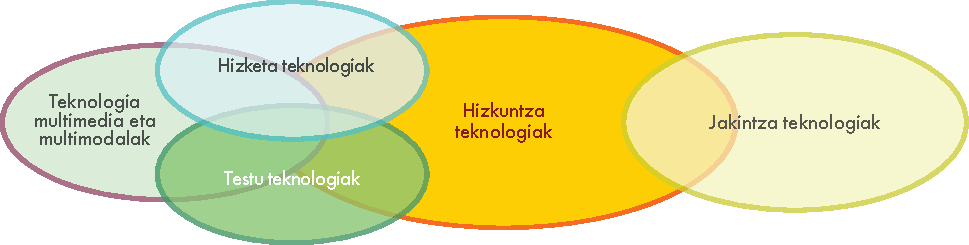
\includegraphics[width=\textwidth]{../_media/basque/language_technologies}
  \caption{Hizkuntza teknologien ingurua}
  \label{fig:ltincontext_eu}
  \colorrule{grey3}{\textwidth}{1.5pt}
\end{figure*}

\subsection[Hizkuntza-teknologia aplikatzeko arkitekturak]{Hizkuntza-teknologia aplikatzeko arkitekturak}
    Hizkuntza prozesatzeko software-aplikazio ohikoenetan, hizkuntzaren hainbat alderdi eta haien zereginak kopiatzen dituzten zenbait osagai egon ohi dira. \ref{fig:textprocessingarch_eu}. irudian, testuak prozesatzeko sistema batean topa dezakegun arkitektura bat ageri da, asko sinplifikatuta. Lehenengo hiru moduluek sarrerako testuaren egitura eta esanahia hartzen dute kontuan:

    \begin{itemize}
      \item Aurretratamendua: datuak garbitu, formatua kendu, sarrerako hizkuntza detektatu eta abar. 
      \item Analisi gramatikala: aditza eta haren objektuak, modifikatzaileak eta abar aurkitu; esaldiaren egitura detektatu.
      \item Analisi semantikoa: desanbiguazioa (“hori” hitzaren zein adiera da egokia testuinguru jakin batean?), anaforak eta erreferentziako adierazpenak (adib. “bera” edo “autoa”) ulertzea; esaldi baten esanahia ordenagailuak irakurtzeko moduan eman.
    \end{itemize}
    Zeregin espezifikoko moduluek era askotako eragiketak egiten dituzte, hala nola sarrerako testu baten laburpen automatikoa, datu-baseko bilaketak eta beste hainbat. Hemen behean, aplikazio-eremu komunak erakutsiko ditugu, eta eremu horietako modulu nagusiak nabarmendu. Hor ere, aplikazioen arkitekturak oso sinplifikatuta eta idealizatuta ageri dira, hizkuntza-teknologiako (HT) aplikazioak edonork ulertzeko moduan azaltzearren. Tresna eta baliabide garrantzitsuenak azpimarratuta daude testuan, eta kapitulu amaierako taulan ere ageri dira. Aplikazio-eremu komunei buruzko ataletan, dagokion euskarazko esparruan lanean ari diren industrien ikuspegi orokor bat ere ematen da.
    
\begin{figure*}[b]
  \colorrule{grey3}{\textwidth}{1.5pt}
  \center
 % \vspace{-5mm} 
 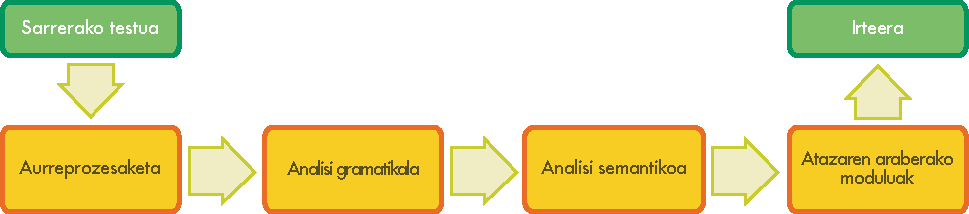
\includegraphics[width=\textwidth]{../_media/basque/text_processing_app_architecture}
  \caption{Testua prozesatzeko aplikazioen ohiko arkitektura}
  \label{fig:textprocessingarch_eu}
  \colorrule{grey3}{\textwidth}{1.5pt}
\end{figure*}

Aplikazio-eremu komunak aurkeztu ondoren, HTen ikerketa eta hezkuntzako egoeraren azalpen labur bat emango dugu, eta, bukatzeko, egin diren eta egiten ari diren ikerketa-programen berri emango dugu. Atal honen amaieran, adituaren ikuspuntutik HTen tresna eta baliabide komunen egoera nolakoa den azalduko dugu, hainbat alderditatik (eskuragarritasuna, heldutasuna eta kalitatea). Taula honek ikuspegi orokor on bat ematen du euskararako HTen egoeraren gainean.  

\subsection{Aplikazio-eremu komunak} 
Atal honetan, HTen tresna eta baliabide garrantzitsuenak aztertu, eta euskarazko HTen jardueren ikuspegi bat emango dugu. Tresna eta baliabide garrantzitsuenak nabarmenduta daude testuan, eta kapitulu amaierako taulan ere ageri dira.

\subsubsection{Hizkuntza-zuzentzailea}
   Testu-prozesadore bat erabili duen edonork egin du topo \textbf{ortografia-zuzentzaile} batekin —ortografia-akatsak markatu eta zuzenketak proposatzen dituen osagaia da—. Ralph Gorin-ek ortografia zuzentzeko lehen programa asmatu zuenetik berrogei urte igaro ondoren, gaur egungo hizkuntza-zuzentzaileek ez dute, besterik gabe, erauzitako hitzen zerrenda bat ortografia zuzeneko hitzen hiztegi batekin alderatzen; gero eta sofistikatuagoak dira. \newline{Morfologia}rako hizkuntzaren menpeko algoritmoez gainera (adibidez, plurala egiteko), batzuk gai dira orain sintaxiarekin lotutako akatsak identifikatzeko, hala nola aditz baten falta edo pertsona edo numeroan subjektuarekin komunztatzen ez duen aditza (“Haiek gutuna idazten ari *\textit{da}”). Alabaina, eskura dauden ortografia-zuzentzaile gehienek (Microsoft Word-ekoa barne) ez dute akatsik aurkituko Jerrold H. Zar-en poema bateko (1992) lehen bertso honetan: 

\hspace{10pt}\textit{Eye have a spelling chequer},

\hspace{10pt}\textit{It came with my Pea Sea}.

\hspace{10pt}\textit{It plane lee marks four my revue}

\hspace{10pt}\textit{Miss Steaks I can knot sea.}

Mota horretako akatsak aurkitzeko, \textbf{testuin\-gurua} aztertu beharra dago maiz, hala nola euskaraz ergatiboa erabili behar den ala ez erabakitzeko orduan:

\hspace{10pt}\textit{Liburua neskak dauka }
 
\hspace{10pt}\textit{Irakurlea neska da.} 
 \begin{figure*}[htb]
  \colorrule{grey3}{\textwidth}{1.5pt}
  %\vspace{-9mm}
  \center
  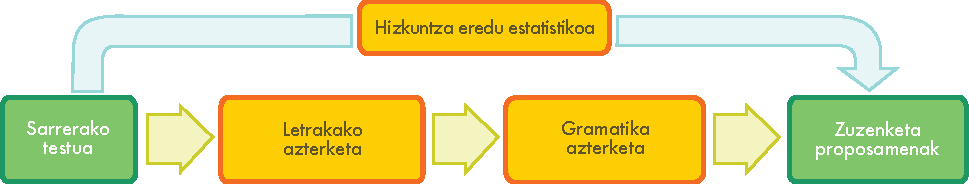
\includegraphics[width=\textwidth]{../_media/basque/language_checking}
  \caption{Hizkuntza azterketa (behean: arauetan oinarritua; goian: estatistikoa)}
  \label{fig:langcheckingaarch_eu}
  \colorrule{grey3}{\textwidth}{1.5pt}
\end{figure*}

Hizkuntza zuzentzailea lortzeko (\ref{fig:langcheckingaarch_eu}), bietakoren bat egin behar da: hizkuntza espezifikoko gramatika-arauak formulatu —trebetasun eta eskulan handia eskatzen du horrek— edo \textbf{hizkuntza-eredu} estatistiko delakoa erabili. Ereduok hitz jakin bat inguru zehatz batean (hots, aurretik eta atzetik dituen hitzak) ateratzeko zer probabilitate dagoen kalkulatzen dute. Adibidez, \textit{neskak dauka} hitz-sekuentzia agertzeko probabilitatea neska dauka agertzekoa baino askoz handiagoa da. Hizkuntza eredu estatistikoa automatikoki atera daiteke hizkuntza-datu zuzenen kantitate handietatik (hots, corpusetatik). Orain arte, ingelesezko hizkuntza-datuetan oinarrituta garatu eta ebaluatu dira metodo horiek. Horrek ez du esan nahi, ordea, euskarara zuzenean transferitu daitezkeenik, euskarak inflexio handiagoa eta morfologia eranskaria du eta. Egia esanda, zailtasun izugarriak daude euskararako hizkuntza-ereduak sortzeko, ezinezkoa baita balizko hitz-forma guztiak biltzea. 

Hizkuntza-zuzentzailea ez da testu-prozesamenduko tresnetan bakarrik erabiltzen; testuak sortzen laguntzeko sistemetan ere erabiltzen da. Produktu teknikoek gora egin duten bezalaxe, dokumentazio teknikoa ere asko ugaritu da azken hamarkadetan. Enpresak, bezeroen aldetik erabilera txarragatiko kexak edo matxuragatiko erreklamazioak (gaizki idatziriko edo ulerturiko jarraibideengatik) jasotzeko beldurrez, dokumentazio teknikoan arreta gehiago jartzen hasi dira, eta nazioarteko merkatuan sartzen ere bai. Hizkuntza naturalaren prozesamenduan egin diren aurrerapenek testuak sortzen laguntzeko softwarea ekarri dute; programa horrek dokumentazio teknikoa jartzen du idazlearen eskura, arau jakin batzuk eta (enpresaren) terminologia-murrizketa batzuk dituzten hitzak eta esaldi-egiturak erabil ditzan. 

\boxtext{Hizkuntza-zuzentzailea ez da testu-prozesamenduko tresnetan bakarrik erabiltzen; testuak sortzen laguntzeko sistemetan ere erabiltzen da}

Euskararako gehien erabiltzen den zuzentzaile ortografikoa Xuxen da \cite{BAS-Nota24}, IXA unibertsitateko ikerkuntza-taldeak (\url{http://ixa.si.ehu.es}) garatu eta Eleka Ingeniaritza Linguistikoa enpresak eskaintzen duena. Zuzentzaile ortografiko hori ez da hiztegi bat erabiltzera mugatzen, ingelesean edo inflexio txikiagoko beste hizkuntza batzuetan egin ohi den moduan. Horren ordez, analisi morfologikoa egiten du. Zuzentzaile ortografiko honen bertsio berrienak gramatika eta estiloa ere zuzentzen ditu. Bertsio horretan, Hizkia \cite{BAS-Nota25} enpresak eta UZEI \cite{BAS-Nota26}  erakundeak garatutako kodea ere badago. 

Zuzentzaile ortografikoetan eta editatzen laguntzeko programetan ez ezik, ordenagailuz lagundutako hizkuntza-ikaskuntzaren esparruan ere garrantzitsua da hizkuntza-zuzentzailea, eta web bilatzaileetara bidalitako dudak automatikoki zuzentzeko ere erabiltzen da; adib. Google-ren "esan nahi zenuen" iradokizunak. 

\subsubsection{Web bilaketak}
   Webeko, intranetetako edo liburutegi digitaletako, bilaketak dira gaur egun gehien erabiltzen den hizkuntza-teknologia, eta, hala ere, gutxi garatuta dago. Google bilatzailea 1998an sortu zen, eta mundu osoko bilaketa guztietatik\% 80tan erabiltzen da gaur egun \cite{BAS-Nota27}. 

Lehenengo bertsio hartatik ez da aldaketa esanguratsurik egon, ez bilaketaren interfazean, ez berreskuratutako emaitzen aurkezpenean. Oraingo bertsioan, Google-k gaizki idatzitako hitzak ortografikoki zuzentzen ditu, eta, 2009an, oinarrizko bilaketa semantikorako ahalmenak gehitu zizkioten bere algoritmo-taldekatzeari \cite{BAS-Nota28} ; hala, bilaketa zehatzagoa egin daiteke, sartutako terminoen esanahia testuinguruan aztertzen da eta. Google-ren arrakastak erakusten du, eskura datu asko eta horiek indexatzeko teknika eraginkorrak izanda, nagusiki estatistiketan oinarritzen den metodo batek emaitza onak eman ditzakeela. 

Dena dela, informazio-eskaera sofistikatuagoetarako, ezagutza linguistiko sakonagoa integratu beharra dago. Ikerketa-laborategietan, makinak irakurtzeko moduko thesaurusak eta hizkuntza-baliabide ontologikoak —adibidez, Wordnet— erabili dituzten esperimentuek hobekuntzak izan dituzte orriak bilaketa terminoen sinonimoen bidez bilatzeko aukerari esker. Aurrerapen horietarako ere hizkuntzaren baliabide espezifikoak behar dira. Euskal Herriko Unibertsitateko IXA ikerkuntza-taldeak EuskalWordnet (BasWN) asmatu du, eta ELRAren bitartez eros daiteke. 

Bilatzaileen hurrengo belaunaldiak hizkuntza-teknologia sofistikatuagoa izan beharko du. Bilaketa-kontsulta galdera bat edo beste mota bateko esaldi bat bada —gako-hitz batzuk izan beharrean—, kontsulta horri erantzun egokiak emateko, esaldi hori sintaktikoki eta semantikoki aztertu behar da, eta indize batek egon behar du dagozkion dokumentuak azkar berreskuratzeko. Adibidez, demagun erabiltzaile batek kontsulta hau egiten duela: “Azken bost urteotan beste enpresa batek xurgatu dituen enpresa guztien zerrenda bat eman iezadazu". Erantzun egokia lortzeko, \textbf{analisi} sintaktikoa egin beharra dago, esaldiaren egitura gramatikala aztertzeko eta jakiteko erabiltzaileak bilatzen duena xurgatuak izan diren enpresak direla, eta ez beste enpresa batzuk xurgatu dituzten enpresak. \textit{Azken bost urteotan} esamoldea ere prozesatu egin behar da, jakiteko zein urteri egiten dien erreferentzia. 

\begin{figure*}[htb]
  \colorrule{grey3}{\textwidth}{1.5pt}
 % \vspace{-9mm}
  \center
  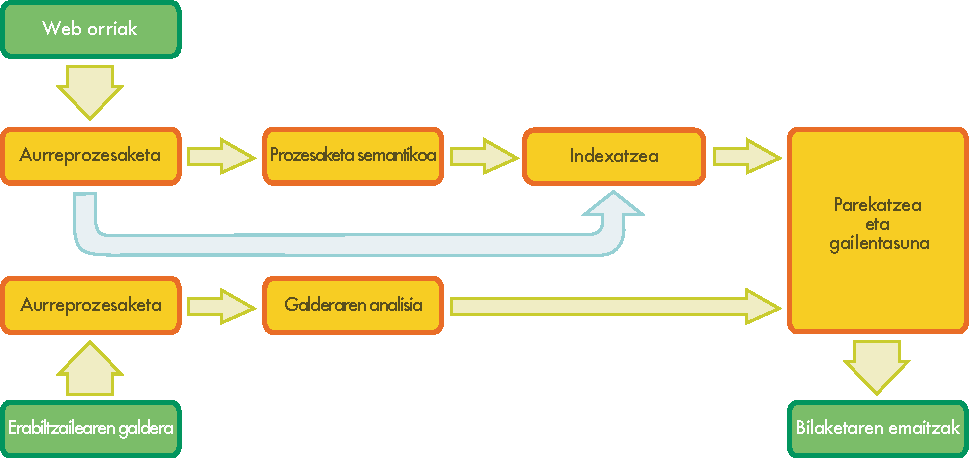
\includegraphics[width=\textwidth]{../_media/basque/web_search_architecture}
  \vspace{-5mm}
  \caption{Web bilaketaren arkitektura}
  \label{fig:websearcharch_eu}
  \colorrule{grey3}{\textwidth}{1.5pt}
\end{figure*}

Azkenik, kontsulta prozesatua egituratu gabeko datu-kantitate handi batekin lotu beharra dago, erabiltzaileak lortu nahi duen informazioa aurkitze aldera. \textbf{Informazio-berreskurapena} esaten zaio horri, eta dokumentu egokiak bilatu eta mailakatzen ditu. Gainera, enpresa-zerrenda bat sortzeko, dokumentu bateko hitz kate bat enpresa-izen bat dela adierazten digun informazioa erauzi behar dugu. Era horretako informazioa \textbf{entitateen izenen ezagutzaile} izenekoen bitartez dago eskuragarri. 

Are zailagoa da bilaketa bat beste hizkuntza batean idatzitako dokumentuekin lotzea. \textbf{Hizkuntzarteko informazio-berresku\-ratzerako}, balizko iturburu-hizkuntza guztietara itzuli behar dugu kontsulta automatikoki, eta berreskuratutako informazioa helburuko hizkuntzara eraman. Testu-formatuez bestelakoetan ematen diren datuen proportzioa handitu den heinean, gero eta gehiago eskatzen dira \textbf{multimedia-informazioa berreskurapenerako} zerbitzuak, hots, irudi-, audio- eta bideo-datuen bilaketak. Audio- eta bideo-fitxategietarako, \textbf{hizketa ezagutzeko} modulua izan behar da, hizketaren edukia testu edo irudikapen fonetiko bihurtzeko, eta, hala, erabiltzailearen kontsultak haiekin lotzeko.

Enpresa horien garapena interes bereziko atariei gehigarriak eta bilatzaile aurreratuak eskaintzean datza, gaiari dagokion semantika erabiliz. Oraindik ere prozesatze-indar handia eskatzen duela eta, bilatzaile horiek \textbf{testu-corpus} nahiko txikietan bakarrik erabil daitezke. Prozesatze-denbora bilatzaile estatistiko arrunt batena baino mila aldiz handiagoa da, gutxienez —adibidez, Google-k eskaintzen duen bilatzailearekin alderatuta—. Bilatzaile horiek eskari handia dute gai espezifikoko domeinuen modelazioan, eta ezinezkoa da mekanismo horiek web-mailan erabiltzea.

\boxtext{Bilatzaileen hurrengo belaunaldiak hizkuntza-teknologia sofistikatuagoa izan beharko du}

Euskal Autonomia Erkidegoan, Eleka Ingeniaritza Linguistikoa enpresa txikia buru-belarri aritu da lanean, euskararako aplikazioak eta webean oinarritutako zerbitzuak garatzen. HTren ikerketa-emaitzak eta baliabideak integratzen dituzte normalean, hala nola IXA taldearen eta Elhuyar Fundazioaren lematizatzaileak eta datu-base lexikalak. Elebila bilatzaile eleaniztunak kontuan hartzen ditu euskararen berezitasunak, eta hainbat hizkuntza-tresna eta -baliabide integratzen ditu, kalitatezko euskarazko emaitzak lortzeko. Beste adibide bat Miatu izeneko tresna da; liburutegi bat da, eta helburu bereziarekin indexatutako datu baseen gainean lematizatzaileak eta analisi morfologikorako beste tresna batzuk erabiliz bilaketak egiteko funtzioak eskaintzen ditu. www.zientzia.net zientziarekin lotutako ataria eta www.ikasbil.net eduki pedagogikoko ataria sortzeko erabili da.
  
\subsubsection{Ahozko interakzioa}
  Erabiltzaile bati grafikoak, teklatua eta saguaren partez ahozko hizkera erabiliz makinekin interakzioan jartzeko aukera ematen dioten interfazeen oinarrian dagoen teknologia da Ahozko Interakzioa. Gaur egun, enpresek beren bezeroei, langileei edo lankideei telefonoz eskaintzen dizkieten automatizazio partzial edo osoko zerbitzuetan erabiltzen dira, normalean, ahotsaren bidezko erabiltzaile-interfazeak (AEI). Lan-arlo hauetan asko erabiltzen dira ahotsaren bidezko erabiltzaile-interfazeak: banketxeak, logistika, garraio publikoa eta telekomunikazioak. Ahozko interakzioaren teknologia gailu jakin batzuen interfazeetan ere egon ohi da —esaterako, autoan txertatuta doazen nabigazio-sistemetan—, eta erabiltzaile-interfaze grafikoen sarrera/irteera modalitateen ordez ahozko hizkera ezartzeko ere erabiltzen dira, Smartphone gailuetan esaterako.


\begin{figure*}[htb]
  \colorrule{grey3}{\textwidth}{1.5pt}
  %\vspace{-9mm}
  \center  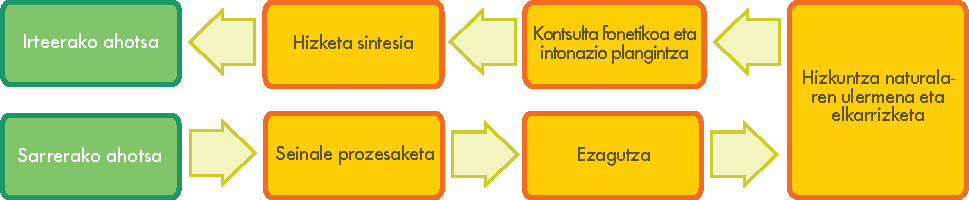
\includegraphics[width=\textwidth]{../_media/basque/simple_speech-based_dialogue_architecture}
  \center
  \caption{Ahots bidezko elkarrizketa sinple baten arkitektura}
  \label{fig:dialoguearch_eu}
  \colorrule{grey3}{\textwidth}{1.5pt}
\end{figure*}

Ahozko interakzioaren oinarrian, lau teknologia hauek daude:

    \begin{itemize}
      \item \textbf{Hizketaren ezagutza} automatikoak: zer hitz esan diren ateratzen du, erabiltzaileak egindako hots-sekuentzia batetik.
      \item Analisi sintaktikoak eta interpretazio semantikoak: erabiltzaile batek esandakoaren egitura sintaktikoa aztertzen du eta interpretatu egiten du sistemaren helburuaren arabera.
      \item Elkarrizketa-kudeaketa: beharrezkoa da erabiltzailearen interakzioko sistema-zatian zer egin zehazteko, behin erabiltzailearen inputa emandakoan eta sistemaren funtzioak kontuan hartuta.
      \item \textbf{Hizketaren sintesirako} teknologia (TTS edo Text-to-Speech): esandako hitz horiek hots bihurtzeko eta erabiltzailearentzako irteera gisa emateko erabiltzen da. 

    \end{itemize}

\boxtext{Erabiltzaile bati ahozko hizkera erabiliz makinekin interakzioan jartzeko aukera ematen dioten interfazeen oinarrian dagoen teknologia da Ahozko Interakzioa}

  Erronkarik handienetarikoa da hizketaren ezagutza automatikoko sistema batek zehaztasun osoz ezagutzea erabiltzaile batek esandako hitzak. Horretarako, bietakoren bat egin behar da: erabiltzailearen balizko esaldiak gako-hitzen sorta mugatu batera murriztu, edo \textbf{hizkuntza-ereduak} sortu eskuz, hizkuntza naturalaren erabiltzailearen esaldi-sorta handia hartzen dutenak. Lehenengoak ahotsaren bidezko erabiltzaile-interfazeen erabilera zorrotz eta zurruna dakar eta erabiltzailearen onarpen eskasa izango du, ziur asko; bestalde, hizkuntza-ereduak sortu, doitu eta zaintzeak asko igo ditzake kostuak. Haatik, hizkuntza-ereduak erabiltzen dituzten eta hasieran erabiltzaile bati zer nahi duen adierazteko malgutasuna ematen dioten —adibidez, “Lagundu zaitzaket?” edo antzeko galderen bidez— ahots bidezko erabiltzaile-interfazeek automatizazio-abiadura hobea dute eta erabiltzaileen onarpen zabalagoa; horregatik, abantailak ikusten zaizkio elkarrizketa-metodo zurrunagoen aldean.


Ahots bidezko erabiltzaile-interfazeen emaitzetarako, enpresek erabiltzen dituzten esaldiak aldez aurretik grabatutakoak izan ohi dira eta hiztun profesionalek esandakoak —ahal izanez gero, enpresakoak bertakoak—. Esaldi estatikoak diren kasuan, hitzen formulazioa erabilera-testuinguru jakin baten edo erabiltzaile horren datu pertsonalen menpekoa ez denean, erabiltzailearen esperientzia ona izango da. Aldiz, esaldi batek zenbat eta eduki dinamikoagoa hartu behar duen kontuan, are txarragoa izango da erabiltzailearen esperientzia,  audio-fitxategi solteak elkarrekin lotzeagatik sortutako prosodia kaskarragoa izango baita. Gaur egungo TTS sistemak, ostera, hobeak dira esaldi dinamikoen naturaltasun prosodikoari dagokionez, nahiz eta oraindik ere hobetu daitezkeen. 

Ahozko interakzioaren teknologiaren merkatuan, azken hamarkadan, teknologia-osagaien arteko interfazeak asko estandarizatu ziren, eta aplikazio jakin baterako software-tresna jakin batzuk sortzeko irizpideak ere agertu ziren. Era berean, merkatua asko indartu da azken hamar urteotan, batez ere hizketaren ezagutza automatikoaren eta TTSen esparruetan. Esparru horietan, G20 herrialdeetako —populazio dezentea eta indar ekonomiko handia duten herrialdeak— merkatu nazionalak mundu osoko bost enpresa baino gutxiagoren eskuetan daude; Europan, Nuance eta Loquendo dira garrantzitsuenak. 2007. urtetik, Eusko Jaurlaritzak emandako babesari esker, Nuanceren produktu-katalogoan sartuta dago euskara. Alabaina, hizketaren ezagutza automatikoaren eskaintza tamaina txiki eta ertaineko hiztegi-aplikazioetara mugatzen da, eta ez da eskaintzen diktaketa-produkturik. TTSrako, emakumezko ahots bakarra eskaintzen da. Espainiako merkatuan, Verbio Speech Technologies \cite{BAS-Nota29}  enpresa kataluniarrak bietarako eskaintzen du euskara, hizketaren ezagutza automatikorako nahiz TTSrako. Euskararako diktaketa-sistema komertzialik ez dago, ordea. 

Elkarrizketa-kudeaketako teknologia eta ezagutzei dagokienez, enpresa nazionalak dira nagusi merkatuetan, ETEak normalean. TTSen Espainiako merkatuan, enpresa gehienak aplikazio sortzaileak dira. Espainiako merkatuko enpresa nagusiak hauek dira: Indsys \cite{BAS-Nota30}  (Intelligent Dialogue Systems), Fonetic \cite{BAS-Nota31}, Ydilo \cite{BAS-Nota32}  eta NaturalVox \cite{BAS-Nota33}. Horietako zenbaitek badute eskaintza mugatu bat euskararentzat. Euskararako doaneko TTS softwarea ere badago, Euskal Herriko Unibertsitateko (UPV/EHU)  Aholab \cite{BAS-Nota34}  ikerkuntza-taldeak eskainia.

Gaur egungo teknologiatik harago begiratuta, aldaketa esanguratsuak egongo dira, Smartphone gailuak hedatu egingo baitira bezeroekiko harremanak kudeatzeko plataforma berri moduan —telefono, Internet eta posta elektronikoarekin batera—. Joera horrek eragina izango du ahozko interakziorako teknologiaren erabileran ere. Alde batetik, epe luzera, behera egingo du telefonian oinarritutako ahotsaren bidezko erabiltzaile-interfazeen eskariak. Bestetik, gero eta gehiago erabiliko da ahozko hizkera Smartphonetarako sarrera-modalitate erabilerraz moduan. Joera hori erakusten dute hiztuna kontuan hartu gabeko hizketaren ezagutzaren zehaztasunean egin diren hobekuntza nabariek —Smartphone-erabiltzaileei zerbitzu zentralizatu moduan jada eskaintzen ari zaizkien ahozko diktaketa-zerbitzuetarako egindakoak—. Ezagutzaren eginkizuna aplikazioen azpiegiturara bideratzeko joera hori ikusita, uste da hizkuntza-teknologia komunen aplikazio espezifikoko erabilerak garrantzia hartuko duela. 

\subsubsection{Itzulpen automatikoa}
  Hizkuntza naturala itzultzeko ordenagailu digitalak erabiltzearen ideia A. D. Booth-ek izan zuen 1946an, eta esparru hori ikertzeko finantzaketa handia egin zen 1950eko hamarkadan, eta,  berriro, 1980eko hamarkadan. Hala ere, \textbf{itzulpen automatikoak} (IA) ez dio oraindik behar bezala erantzun hasierako urteetan sortu zuen itxaropenari. 

\boxtext{Itzulpen Automatikoak, bere oinarrizko mailan, hizkuntza natural bateko hitzak kendu eta beste batekoak jarri besterik ez du egiten}

\begin{figure*}[htb]
  \colorrule{grey3}{\textwidth}{1.5pt}
 % \vspace{-21mm}
  \center
  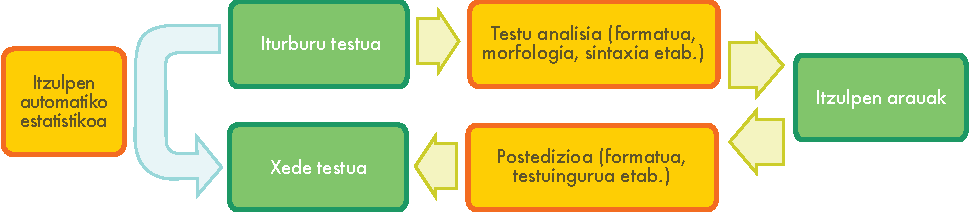
\includegraphics[width=\textwidth]{../_media/basque/machine_translation}
  \vspace{-2mm}
  \caption{Itzulpen automatikoa (ezkerrean: estatistikoa, eskuinean: arau bidezkoa)}
  \label{fig:mtarch_eu}
  \colorrule{grey3}{\textwidth}{1.5pt}
\end{figure*}

IAk, bere oinarrizko mailan, hizkuntza natural bateko hitzak kendu eta beste batekoak jarri besterik ez du egiten. Hori baliagarria izan daiteke esapide gutxiko hizkera oso mugatua darabilten esparruetan, hala nola eguraldi-iragarpenetan. Estandarizazio gutxiagoko testuak ondo itzultzeko, ordea, testu-unitate handiagoak (esapideak, esaldiak eta pasarte osoak ere bai) xede-hizkuntzako baliokide aproposenekin lotu behar dira. Horko zailtasunik handiena giza hizkuntzaren anbiguotasuna da, erronkak ezartzen baititu hainbat mailatan; esaterako, \textbf{adiera desanbiguazioa} lexiko-mailan (“Jaguar” hitzak autoari edo animaliari egin diezaioke erreferentzia) edo beste maila batzuetan, adibidez:

\textit{Egon garenetan ez dugu topatu}

\textit{[Egon garen aldietan ez dugu topatu] edo} 

\textit{[Egon garen tokietan ez dugu topatu]}

\textit{Aitak semeari bere bizikleta eman dio}

\textit{[Aitarena ala semearena?]}

Halakoak konpontzeko modu bat hizkuntza-arauetan oinarritzen da. Familia bereko hizkuntzekin ari bagara lanean, beharbada zuzeneko itzulpena egin daiteke bigarren adibidearen gisako perpausetan. Baina, sarritan, arauan oinarritutako sistemek (edo ezagutzak gidaturikoek) sarrera-testua aztertu eta tarteko adierazpide sinboliko bat sortzen dute, eta hortik sortzen da xede-hizkuntzako testua. Metodo horiek arrakasta izan dezaten, hiztegi handiak izan behar dituzte, informazio morfologiko, sintaktiko eta semantikoa biltzen dutenak, eta gramatika-arauen bilduma handia, hizkuntzalari aditu batek tentuz diseinaturikoa.

1980ko hamarkadaren amaieratik hasita, ordenagailua garrantzia hartuz eta merkatuz joan zen heinean, gero eta jakin-min handiagoa pizten zuten IArako eredu estatistikoek. Eredu estatistiko horien parametroak testu elebidunen corpusen analisitik atera dira; hor dugu, esaterako, Europarl corpus paraleloa, Europako Legebiltzarraren aktak 11 hizkuntza europarretan ematen dituena. Datu nahikoa izanez gero, IA estatistikoa nahiko baliagarria da atzerriko hizkuntzan idatzitako testu baten gutxi gorabeherako esanahia ateratzeko. Alabaina, ezagutzak gidaturiko sistemekin alderatuta IA estatistikoak (edo datuek gidaturikoak) duen desabantaila da emaitza agramatikalak sortzen dituela maiz. Bestalde, datuek gidaturiko IAk, gramatika idazteko giza ahalegin txikiagoa behar izateaz gainera, badu beste abantaila bat: ezagutzak gidaturiko sistemei ihes egiten dizkieten berezitasunak ondo trata ditzake, esapideak kasurako. 

Ezagutzak gidaturiko IAren eta datuek gidaturiko IAren indarguneak eta ahulguneak elkarrekiko osagarriak direnez, bietako metodologiak nahasten dituzten metodo hibridoetara jotzen dute ikerlari guztiek gaur egun. Hori egiteko era bat baino gehiago daude. Batean, bi sistemak erabiltzen dira —ezagutzak gidaturikoa eta datuek gidaturikoa—, eta hautapen-modulu batek erabakitzen du zein den esaldi bakoitzaren irteerako esaldi onena. Esaldi luzeetarako, ordea, ez du topatzen emaitza egokirik. Konponbide hobea da irteera askotako esaldien zatirik onenak elkartzea; hori nahiko zaila izan daiteke, askotariko aukerei dagozkien atalak ez baitira beti agerikoak eta lerrokatu egin behar izaten baitira. 

Euskararentzat, IA bereziki zaila da. Euskara hizkuntza eranskaria, morfologia aberatsekoa eta flexio maila handikoa izanda, hiztegiaren analisia eta hiztegi-estaldura zailagoa da. Gainera, esaldiko osagaien hurrenkera dela bide, lan nekeza da \textbf{corpus paraleloak} kudeatzea. 

\textit{Matxin} transferentzian oinarritutako IA sistema bat da, gaztelaniatik euskararakoa, IXA taldeak Euskal Herriko Unibertsitatean garatutakoa.  Irekia da, berrerabilgarria, eta euskarri elkarreragingarria eskaintzen du beste hizkuntza bikoteentzat ere (matxin.sourceforge.org). Kode irekiko beste programa batzuk erabiltzen ditu, hala nola Freeling, eta euskararen morfologia berrerabiltzen du morfologia sorkuntzarako. IXA taldeak Itzulpen Automatiko Estatistikoko sistema bat ere sortu du euskara eta gaztelaniarako, hitzen segmentazioa eta berrordenaketa egiten duena (EUSMT). IA sistema horiek garatzeko, lankidetza estua dago unibertsitateko ikerkuntza-taldearen, Eleka Ingeniaritza Linguistikoa enpresa txikiaren eta Elhuyar Fundazioaren artean —azken horrek hizkuntza-baliabide asko jartzen ditu—. Eleka enpresak Batua-Bizkaiera bihurtzailea ere atera du. Alacanteko Unibertsitateko Transducens taldeak ere garatu du euskaratik gaztelaniara itzultzeko hasierako sistema bat, Apertium plataforma erabiltzen duena. Google Itzultzaileak alfa bertsio bat eskaintzen du euskararentzat.

Lucy Software enpresak —IAko aplikazioen sortzaile garrantzitsuenetakoa da nazioartean— filial bat dauka Espainian, Lucy Iberica \cite{BAS-Nota35}, lehen Trans\-len\-dium zena. Eusko Jaurlaritzak enpresa hori hautatu zuen 2008an, gaztelaniatik euskararako itzulpen-sistema bat sortzeko, eta 2011an berriro hautatu zuen lan horrekin jarrai zezan. 

Erabiltzailearekiko espezifikoa den terminologia eta lan-prozesuen integrazioa behar bezala egokituz gero, oro har, uste da IAren erabilerak produktibitatea asko hobetu dezakeela. Halaber, IA sistemen kalitatea oraindik asko hobetu daitekeela uste da. Hainbat erronka daude oraindik; besteak beste, hizkuntza-baliabideak esparru edo erabiltzaile-talde jakin batera egokitzea eta lehendik dauden prozesuetan integratzea, terminoen datu-baseekin eta itzulpen-memoriekin batera. Gainera, hizkuntza-bikote asko falta dira oraindik.

\begin{figure*}[tb]
  \centering
  \setlength{\tabcolsep}{0.17em}
  \small
  \begin{tabular}{>{\columncolor{corange1}}cccccccccccccccccccccccc}
    & \multicolumn{22}{>{\columncolor{corange1}}c}{Xede hizkuntza-- \textcolor{grey1}{Target language}}\\\addlinespace[{-.009cm}]
    \rowcolor{corange1}  & EN & BG & DE & CS & DA & EL & ES & ET & FI & FR & HU & IT & LT & LV & MT & NL & PL & PT & RO & SK & SL & SV\\
    EN & -- & \textcolor{blue}{40.5} & \textcolor{blue}{46.8} & \textcolor{green2}{52.6} & \textcolor{green2}{50.0} & \textcolor{blue}{41.0} & \textcolor{green2}{55.2} & \textcolor{purple}{34.8} & \textcolor{purple}{38.6} & \textcolor{green2}{50.1} & \textcolor{purple}{37.2} & \textcolor{green2}{50.4} & \textcolor{purple}{39.6} & \textcolor{blue}{43.4} & \textcolor{purple}{39.8} & \textcolor{green2}{52.3} & \textcolor{blue}{49.2} & \textcolor{green2}{55.0} & \textcolor{blue}{49.0} & \textcolor{blue}{44.7} & \textcolor{green2}{50.7} & \textcolor{green2}{52.0}\\
    BG & \textcolor{green}{61.3} & -- & \textcolor{purple}{38.7} & \textcolor{purple}{39.4} & \textcolor{purple}{39.6} & \textcolor{purple}{34.5} & \textcolor{blue}{46.9} & \textcolor{red3}{25.5} & \textcolor{red3}{26.7} & \textcolor{blue}{42.4} & \textcolor{red3}{22.0} & \textcolor{blue}{43.5} & \textcolor{red3}{29.3} & \textcolor{red3}{29.1} & \textcolor{red3}{25.9} & \textcolor{blue}{44.9} & \textcolor{purple}{35.1} & \textcolor{blue}{45.9} & \textcolor{purple}{36.8} & \textcolor{purple}{34.1} & \textcolor{purple}{34.1} & \textcolor{purple}{39.9}\\
    DE & \textcolor{green2}{53.6} & \textcolor{red3}{26.3} & -- & \textcolor{purple}{35.4} & \textcolor{blue}{43.1} & \textcolor{purple}{32.8} & \textcolor{blue}{47.1} & \textcolor{red3}{26.7} & \textcolor{red3}{29.5} & \textcolor{purple}{39.4} & \textcolor{red3}{27.6} & \textcolor{blue}{42.7} & \textcolor{red3}{27.6} & \textcolor{purple}{30.3} & \textcolor{red2}{19.8} & \textcolor{green2}{50.2} & \textcolor{purple}{30.2} & \textcolor{blue}{44.1} & \textcolor{purple}{30.7} & \textcolor{red3}{29.4} & \textcolor{purple}{31.4} & \textcolor{blue}{41.2}\\
    CS & \textcolor{green2}{58.4} & \textcolor{purple}{32.0} & \textcolor{blue}{42.6} & -- & \textcolor{blue}{43.6} & \textcolor{purple}{34.6} & \textcolor{blue}{48.9} & \textcolor{purple}{30.7} & \textcolor{purple}{30.5} & \textcolor{blue}{41.6} & \textcolor{red3}{27.4} & \textcolor{blue}{44.3} & \textcolor{purple}{34.5} & \textcolor{purple}{35.8} & \textcolor{red3}{26.3} & \textcolor{blue}{46.5} & \textcolor{purple}{39.2} & \textcolor{blue}{45.7} & \textcolor{purple}{36.5} & \textcolor{blue}{43.6} & \textcolor{blue}{41.3} & \textcolor{blue}{42.9}\\
    DA & \textcolor{green2}{57.6} & \textcolor{red3}{28.7} & \textcolor{blue}{44.1} & \textcolor{purple}{35.7} & -- & \textcolor{purple}{34.3} & \textcolor{blue}{47.5} & \textcolor{red3}{27.8} & \textcolor{purple}{31.6} & \textcolor{blue}{41.3} & \textcolor{red3}{24.2} & \textcolor{blue}{43.8} & \textcolor{red3}{29.7} & \textcolor{purple}{32.9} & \textcolor{red3}{21.1} & \textcolor{blue}{48.5} & \textcolor{purple}{34.3} & \textcolor{blue}{45.4} & \textcolor{purple}{33.9} & \textcolor{purple}{33.0} & \textcolor{purple}{36.2} & \textcolor{blue}{47.2}\\
    EL & \textcolor{green2}{59.5} & \textcolor{purple}{32.4} & \textcolor{blue}{43.1} & \textcolor{purple}{37.7} & \textcolor{blue}{44.5} & -- & \textcolor{green2}{54.0} & \textcolor{red3}{26.5} & \textcolor{red3}{29.0} & \textcolor{blue}{48.3} & \textcolor{red3}{23.7} & \textcolor{blue}{49.6} & \textcolor{red3}{29.0} & \textcolor{purple}{32.6} & \textcolor{red3}{23.8} & \textcolor{blue}{48.9} & \textcolor{purple}{34.2} & \textcolor{green2}{52.5} & \textcolor{purple}{37.2} & \textcolor{purple}{33.1} & \textcolor{purple}{36.3} & \textcolor{blue}{43.3}\\
    ES & \textcolor{green}{60.0} & \textcolor{purple}{31.1} & \textcolor{blue}{42.7} & \textcolor{purple}{37.5} & \textcolor{blue}{44.4} & \textcolor{purple}{39.4} & -- & \textcolor{red3}{25.4} & \textcolor{red3}{28.5} & \textcolor{green2}{51.3} & \textcolor{red3}{24.0} & \textcolor{green2}{51.7} & \textcolor{red3}{26.8} & \textcolor{purple}{30.5} & \textcolor{red3}{24.6} & \textcolor{blue}{48.8} & \textcolor{purple}{33.9} & \textcolor{green2}{57.3} & \textcolor{purple}{38.1} & \textcolor{purple}{31.7} & \textcolor{purple}{33.9} & \textcolor{blue}{43.7}\\
    ET & \textcolor{green2}{52.0} & \textcolor{red3}{24.6} & \textcolor{purple}{37.3} & \textcolor{purple}{35.2} & \textcolor{purple}{37.8} & \textcolor{red3}{28.2} & \textcolor{blue}{40.4} & -- & \textcolor{purple}{37.7} & \textcolor{purple}{33.4} & \textcolor{purple}{30.9} & \textcolor{purple}{37.0} & \textcolor{purple}{35.0} & \textcolor{purple}{36.9} & \textcolor{red3}{20.5} & \textcolor{blue}{41.3} & \textcolor{purple}{32.0} & \textcolor{purple}{37.8} & \textcolor{red3}{28.0} & \textcolor{purple}{30.6} & \textcolor{purple}{32.9} & \textcolor{purple}{37.3}\\
    FI & \textcolor{blue}{49.3} & \textcolor{red3}{23.2} & \textcolor{purple}{36.0} & \textcolor{purple}{32.0} & \textcolor{purple}{37.9} & \textcolor{red3}{27.2} & \textcolor{purple}{39.7} & \textcolor{purple}{34.9} & -- & \textcolor{red3}{29.5} & \textcolor{red3}{27.2} & \textcolor{purple}{36.6} & \textcolor{purple}{30.5} & \textcolor{purple}{32.5} & \textcolor{red2}{19.4} & \textcolor{blue}{40.6} & \textcolor{red3}{28.8} & \textcolor{purple}{37.5} & \textcolor{red3}{26.5} & \textcolor{red3}{27.3} & \textcolor{red3}{28.2} & \textcolor{purple}{37.6}\\
    FR & \textcolor{green}{64.0} & \textcolor{purple}{34.5} & \textcolor{blue}{45.1} & \textcolor{purple}{39.5} & \textcolor{blue}{47.4} & \textcolor{blue}{42.8} & \textcolor{green}{60.9} & \textcolor{red3}{26.7} & \textcolor{purple}{30.0} & -- & \textcolor{red3}{25.5} & \textcolor{green2}{56.1} & \textcolor{red3}{28.3} & \textcolor{purple}{31.9} & \textcolor{red3}{25.3} & \textcolor{green2}{51.6} & \textcolor{purple}{35.7} & \textcolor{green}{61.0} & \textcolor{blue}{43.8} & \textcolor{purple}{33.1} & \textcolor{purple}{35.6} & \textcolor{blue}{45.8}\\
    HU & \textcolor{blue}{48.0} & \textcolor{red3}{24.7} & \textcolor{purple}{34.3} & \textcolor{purple}{30.0} & \textcolor{purple}{33.0} & \textcolor{red3}{25.5} & \textcolor{purple}{34.1} & \textcolor{red3}{29.6} & \textcolor{red3}{29.4} & \textcolor{purple}{30.7} & -- & \textcolor{purple}{33.5} & \textcolor{red3}{29.6} & \textcolor{purple}{31.9} & \textcolor{red2}{18.1} & \textcolor{purple}{36.1} & \textcolor{red3}{29.8} & \textcolor{purple}{34.2} & \textcolor{red3}{25.7} & \textcolor{red3}{25.6} & \textcolor{red3}{28.2} & \textcolor{purple}{30.5}\\
    IT & \textcolor{green}{61.0} & \textcolor{purple}{32.1} & \textcolor{blue}{44.3} & \textcolor{purple}{38.9} & \textcolor{blue}{45.8} & \textcolor{blue}{40.6} & \textcolor{red3}{26.9} & \textcolor{red3}{25.0} & \textcolor{red3}{29.7} & \textcolor{green2}{52.7} & \textcolor{red3}{24.2} & -- & \textcolor{red3}{29.4} & \textcolor{purple}{32.6} & \textcolor{red3}{24.6} & \textcolor{green2}{50.5} & \textcolor{purple}{35.2} & \textcolor{green2}{56.5} & \textcolor{purple}{39.3} & \textcolor{purple}{32.5} & \textcolor{purple}{34.7} & \textcolor{blue}{44.3}\\
    LT & \textcolor{green2}{51.8} & \textcolor{red3}{27.6} & \textcolor{purple}{33.9} & \textcolor{purple}{37.0} & \textcolor{purple}{36.8} & \textcolor{red3}{26.5} & \textcolor{red3}{21.1} & \textcolor{purple}{34.2} & \textcolor{purple}{32.0} & \textcolor{purple}{34.4} & \textcolor{red3}{28.5} & \textcolor{purple}{36.8} & -- & \textcolor{blue}{40.1} & \textcolor{red3}{22.2} & \textcolor{purple}{38.1} & \textcolor{purple}{31.6} & \textcolor{purple}{31.6} & \textcolor{red3}{29.3} & \textcolor{purple}{31.8} & \textcolor{purple}{35.3} & \textcolor{purple}{35.3}\\
    LV & \textcolor{green2}{54.0} & \textcolor{red3}{29.1} & \textcolor{purple}{35.0} & \textcolor{purple}{37.8} & \textcolor{purple}{38.5} & \textcolor{red3}{29.7} & \textcolor{red2}{8.0} & \textcolor{purple}{34.2} & \textcolor{purple}{32.4} & \textcolor{purple}{35.6} & \textcolor{red3}{29.3} & \textcolor{purple}{38.9} & \textcolor{purple}{38.4} & -- & \textcolor{red3}{23.3} & \textcolor{blue}{41.5} & \textcolor{purple}{34.4} & \textcolor{purple}{39.6} & \textcolor{purple}{31.0} & \textcolor{purple}{33.3} & \textcolor{purple}{37.1} & \textcolor{purple}{38.0}\\
    MT & \textcolor{green}{72.1} & \textcolor{purple}{32.2} & \textcolor{purple}{37.2} & \textcolor{purple}{37.9} & \textcolor{purple}{38.9} & \textcolor{purple}{33.7} & \textcolor{blue}{48.7} & \textcolor{red3}{26.9} & \textcolor{red3}{25.8} & \textcolor{blue}{42.4} & \textcolor{red3}{22.4} & \textcolor{blue}{43.7} & \textcolor{purple}{30.2} & \textcolor{purple}{33.2} & -- & \textcolor{blue}{44.0} & \textcolor{purple}{37.1} & \textcolor{blue}{45.9} & \textcolor{purple}{38.9} & \textcolor{purple}{35.8} & \textcolor{blue}{40.0} & \textcolor{blue}{41.6}\\
    NL & \textcolor{green2}{56.9} & \textcolor{red3}{29.3} & \textcolor{blue}{46.9} & \textcolor{purple}{37.0} & \textcolor{blue}{45.4} & \textcolor{purple}{35.3} & \textcolor{blue}{49.7} & \textcolor{red3}{27.5} & \textcolor{red3}{29.8} & \textcolor{blue}{43.4} & \textcolor{red3}{25.3} & \textcolor{blue}{44.5} & \textcolor{red3}{28.6} & \textcolor{purple}{31.7} & \textcolor{red3}{22.0} & -- & \textcolor{purple}{32.0} & \textcolor{blue}{47.7} & \textcolor{purple}{33.0} & \textcolor{purple}{30.1} & \textcolor{purple}{34.6} & \textcolor{blue}{43.6}\\
    PL & \textcolor{green}{60.8} & \textcolor{purple}{31.5} & \textcolor{blue}{40.2} & \textcolor{blue}{44.2} & \textcolor{blue}{42.1} & \textcolor{purple}{34.2} & \textcolor{blue}{46.2} & \textcolor{red3}{29.2} & \textcolor{red3}{29.0} & \textcolor{blue}{40.0} & \textcolor{red3}{24.5} & \textcolor{blue}{43.2} & \textcolor{purple}{33.2} & \textcolor{purple}{35.6} & \textcolor{red3}{27.9} & \textcolor{blue}{44.8} & -- & \textcolor{blue}{44.1} & \textcolor{purple}{38.2} & \textcolor{purple}{38.2} & \textcolor{purple}{39.8} & \textcolor{blue}{42.1}\\
    PT & \textcolor{green}{60.7} & \textcolor{purple}{31.4} & \textcolor{blue}{42.9} & \textcolor{purple}{38.4} & \textcolor{blue}{42.8} & \textcolor{blue}{40.2} & \textcolor{green}{60.7} & \textcolor{red3}{26.4} & \textcolor{red3}{29.2} & \textcolor{green2}{53.2} & \textcolor{red3}{23.8} & \textcolor{green2}{52.8} & \textcolor{red3}{28.0} & \textcolor{purple}{31.5} & \textcolor{red3}{24.8} & \textcolor{blue}{49.3} & \textcolor{purple}{34.5} & -- & \textcolor{purple}{39.4} & \textcolor{purple}{32.1} & \textcolor{purple}{34.4} & \textcolor{blue}{43.9}\\
    RO & \textcolor{green}{60.8} & \textcolor{purple}{33.1} & \textcolor{purple}{38.5} & \textcolor{purple}{37.8} & \textcolor{blue}{40.3} & \textcolor{purple}{35.6} & \textcolor{green2}{50.4} & \textcolor{red3}{24.6} & \textcolor{red3}{26.2} & \textcolor{blue}{46.5} & \textcolor{red3}{25.0} & \textcolor{blue}{44.8} & \textcolor{red3}{28.4} & \textcolor{red3}{29.9} & \textcolor{red3}{28.7} & \textcolor{blue}{43.0} & \textcolor{purple}{35.8} & \textcolor{blue}{48.5} & -- & \textcolor{purple}{31.5} & \textcolor{purple}{35.1} & \textcolor{purple}{39.4}\\
    SK & \textcolor{green}{60.8} & \textcolor{purple}{32.6} & \textcolor{purple}{39.4} & \textcolor{blue}{48.1} & \textcolor{blue}{41.0} & \textcolor{purple}{33.3} & \textcolor{blue}{46.2} & \textcolor{red3}{29.8} & \textcolor{red3}{28.4} & \textcolor{purple}{39.4} & \textcolor{red3}{27.4} & \textcolor{blue}{41.8} & \textcolor{purple}{33.8} & \textcolor{purple}{36.7} & \textcolor{red3}{28.5} & \textcolor{blue}{44.4} & \textcolor{purple}{39.0} & \textcolor{blue}{43.3} & \textcolor{purple}{35.3} & -- & \textcolor{blue}{42.6} & \textcolor{blue}{41.8}\\
    SL & \textcolor{green}{61.0} & \textcolor{purple}{33.1} & \textcolor{purple}{37.9} & \textcolor{blue}{43.5} & \textcolor{blue}{42.6} & \textcolor{purple}{34.0} & \textcolor{blue}{47.0} & \textcolor{purple}{31.1} & \textcolor{red3}{28.8} & \textcolor{purple}{38.2} & \textcolor{red3}{25.7} & \textcolor{blue}{42.3} & \textcolor{purple}{34.6} & \textcolor{purple}{37.3} & \textcolor{purple}{30.0} & \textcolor{blue}{45.9} & \textcolor{purple}{38.2} & \textcolor{blue}{44.1} & \textcolor{purple}{35.8} & \textcolor{purple}{38.9} & -- & \textcolor{blue}{42.7}\\
    SV & \textcolor{green2}{58.5} & \textcolor{red3}{26.9} & \textcolor{blue}{41.0} & \textcolor{purple}{35.6} & \textcolor{blue}{46.6} & \textcolor{purple}{33.3} & \textcolor{blue}{46.6} & \textcolor{red3}{27.4} & \textcolor{purple}{30.9} & \textcolor{purple}{38.9} & \textcolor{red3}{22.7} & \textcolor{blue}{42.0} & \textcolor{red3}{28.2} & \textcolor{purple}{31.0} & \textcolor{red3}{23.7} & \textcolor{blue}{45.6} & \textcolor{purple}{32.2} & \textcolor{blue}{44.2} & \textcolor{purple}{32.7} & \textcolor{purple}{31.3} & \textcolor{purple}{33.5} & --\\
    \end{tabular}
  \caption{22 hizkuntza europear arteko itzulpen automatikoa -- \textcolor{grey1}{Machine translation between 22 EU-languages \cite{euro1}}}
  \label{fig:euromatrix_en}
\end{figure*}


\subsection{Beste erabilera-eremu batzuk}

   Hizkuntza-teknologiako aplikazioak sortzeko, era askotako lanak egin behar dira, eta, batzuetan, lan horiek ez dira agertzen erabiltzailearekiko elkarreraginean, baina zerbitzu-funtzio garrantzitsuak betetzen dituzte sistemaren “erraietan”. Horregatik, ikergai garrantzitsuak dira, eta esparru akademikoko hizkuntzalaritza konputazionalaren barruko banakako diziplinak dira orain. 

Galderei erantzutea ikerketa-arlo bizia da orain; corpus etiketatuak egin dira horretarako eta lehiaketa zientifikoak antolatu dira. Ideia da gako-hitzetan oinarritutako bilaketa atzean uztea (bilatzaileak garrantzitsuak izan daitezkeen dokumentuen sorta handi bat ematen du), eta bilaketa zehatza egin ahal izatea (erabiltzaileak galdera zehatz bat egiten du, eta sistemak erantzun bakar bat ematen dio):

\begin{itemize}
\item[] \textit{Question: Zer adin zuen Neil Amstrongek ilargira iritsi zenean?}  %%Please translate "Question"
\item[] \textit{Answer: 38.}  %%Please translate "Answer"
\end{itemize}

Argi dago hori lehen aipatu dugun web-bilaketaren esparru komunarekin dagoela lotuta, baina, galderei erantzutea, gaur egun termino zabala da eta hainbat zalantza sortzen ditu, hala nola “Zer galdera mota ezberdindu behar lirateke eta nola tratatu behar lirateke”, “Nola azter eta erka daitezke erantzuna izan dezaketen dokumentuak” (bat ez datozen erantzunak eman ditzakete?) eta “Nola erauz daiteke informazio espezifikoa (erantzuna) testu batetik testuingurua gehiegi baztertu gabe?”. 

Horrek lotura du informazio-erauzketa (IE) delako lanarekin ere; garrantzi eta eragin handiko alorra izan zen hori 1990eko hamarkadaren hasieran, hizkuntzalaritza konputazionalaren barruan "aldaketa estatistikoa" gertatu zen garaian. IEren xedea da dokumentu mota espezifikoetan informazio espezifikoa aurkitzea; adibidez, egunkarietako pasarteetan kontatzen diren enpresa-xurgatzeetan partaide nagusiak zein diren aurkitzea. Landutako beste alor bat terroristen erasoei buruzko albisteena da; horietan, erasoaren egilea, helburua, ordua, tokia eta ondorioak jasotzen dituen txantiloi batera pasatzea da arazoa. Esparru espezifikoko txantiloiak betetzeko gaitasuna IEren bereizgarri nagusia da, eta, horregatik, “atzeko” teknologiaren beste adibide bat da; ondo zedarritutako ikerketa-eremuak ditu, baina, erabilgarria izan dadin, aplikazio-inguru egoki batean txertatu behar da. 

\boxtext{Hizkuntza-teknologiako aplikazioek zerbitzu-funtzio garrantzitsuak beetetzen dituzte software-sistema handiagoen baitan}

Bi “mugako” eremu daude: \textbf{testu-labur\-pe\-nak} eta \textbf{testu-sorkuntza}; batzuetan, aplikazio autonomoak dira, eta, beste batzuetan, azpiko aplikazio laguntzaileak. Testu-laburpenak, agerikoa den moduan, testu luze bat laburtzeko lanari egiten dio erreferentzia, eta MS Word-en barruko funtzio moduan eskaintzen da, esaterako. Batez ere estatistiketan oinarrituta egiten du lan; lehenik, testu bateko hitz “garrantzitsuak” aurkitzen ditu (adibidez, testuan oso maiz eta hizkuntzaren erabilera orokorrean askoz gutxiagotan agertzen diren hitzak), eta, gero, hitz garrantzitsu asko dituzten esaldiak detektatzen ditu. Esaldi horiek dokumentuan markatu edo handik erauzi egiten ditu, eta laburpena egiteko erabiltzen ditu. Zeregin horretan —eta horixe da bere zeregin nagusia—, testu-laburpena eta esaldi-erauzketa gauza bera dira: testua txikiagotu egiten da bere esaldien azpimultzo batera. Testu-laburpenerako tresna komertzial guztiek ideia horixe erabiltzen dute. Zertxobait ikertu den beste metodo bat laburpenean esaldi berriak sartzea da; hots, jatorrizko testuan forma horretan agertu beharrik ez duten esaldiez osaturiko laburpena egitea. Horretarako, testua sakonagotik ulertu behar da, eta, beraz, ez da horren metodo sendoa. Azken batean, testu-sortzaile bat normalean ez da izaten aplikazio autonomo bat, software handiagoko batean txertatutako aplikazioa baizik; adibidez, informazio klinikoaren sistemetan, pazienteen datuak bildu, gorde eta prozesatu egiten dira, eta txostena sortzea da sisteman txertatutako testu-sortzailearen funtzioetako bat. 

\boxtext{Euskararako eta, halaber, hizkuntza gehienetarako, testu-teknologia gehienetako ikerketa ez dago ingeleserako bezain garatua}

Ikerkuntza-eremu horiek guztiak ez daude ingeleserako bezainbeste garatuta euskararako. Bada, ingelesean, hainbat eta hainbat lehiaketa ireki egin dira galderei erantzutearen, informazio-erauzketaren eta testu-laburpenen esparruetan, Estatu Batuetako DARPA eta NISTek antolatuta. Horrek aurrerapen handiak ekarri ditu esparruan, baina jomuga ingelesa izan da beti; lehiaketa batzuetan sartu izan dira hainbat hizkuntza, baina euskara ez da inoiz horietako bat izan. Hori dela eta, corpus etiketatu edo baliabide gutxi daude eskuragarri zeregin horietarako. Testu-laburpenetarako sistemak, metodo estatistikoak bakarrik erabiltzen dituztenean, hizkuntzaren mendekoak dira, neurri handi batean, eta, beraz, zenbait ikerketa-prototipo daude eskuragarri. Testu-sorkuntzarako, osagai berrerabilgarriak gainazala egiteko moduluetara (“sorkuntza-gramatiketara”) mugatuta egon izan dira; hor ere, eskura dauden software gehienak ingeleserako dira. 

\subsection{Hizkuntza-teknologia hezkuntzan}
   Hizkuntza-teknologia diziplinarteko alorra da, eta hainbat adituren lana hartzen du; besteak beste, hizkuntzalariak, informatikariak, matematikariak, filosofoak, psikolinguistak eta neurozientzialariak. Hortaz, gaur egun, Espainian, hizkuntzalari konputazional izateko oinarrizko prestakuntza filologia edo hizkuntzalaritzako gradu baten barruan emango da, beharbada —irakasgai komunen artean hizkuntzalaritza konputazionala ematen bada—, edo informatika-fakultatean, bestela. Lehen aukera eskaintzen duten unibertsitateak hauek dira: Universitat de Barcelona, Universitat Pompeu Fabra, Universitat Oberta de Catalunya eta Universidade de Vigo. Hizkuntzalaritza konputazionala irakasgaitzat ematen duten informatika-fakultate nagusiak, berriz, beste hauek dira: Universidad Politécnica de Madrid, Universidad Carlos III, Universidad Autónoma de Madrid, Universitat d’Alacant, Universidad Nacional de Educación a Distancia eta Euskal Herriko Unibertsitatea. Bi aukerak eskaintzen dituenik ere bada: Universidad Complutense.

Graduondoko ikastaroek helburu zehatzagoa duen prestakuntza profesionala eskaintzen dute. Doktore-ikastaro batzuetan ematen dira hizkuntzaren eta hizketaren prozesamenduarekin lotutako masterrak eta irakasgaiak. Euskal Herriko Unibertsitateak hizkuntzaren prozesamenduari buruzko doktoretza-ikastaro oso bat eskaintzen du, euskara hutsean ere ikas daitekeena. Beste master edo doktoretza-ikastaro batzuetako ikasleei ere eskaintzen zaizkie hizkuntza-teknologiako moduluak, hizketaren prozesamendua batik bat (adib. EHUren Sare Mugikorretako Informazio- eta Komunikazio-teknologiak masterreko ikasleei). 

Euskal Autonomia Erkidegoko hiru unibertsitateetan banatuta dauden zenbait ikerketa-talde ari dira gai hauek lantzen: hizketaren prozesamendua, hizketaren sintesia eta bihurketa, hizketaren eta hiztunaren ezagutza, hizkuntzaren ezagutza, hizkuntza naturalaren prozesamendua, testutik testurako itzulpena eta hizketatik hizketarako itzulpena. Guztiak dira Hizkuntza Naturalaren Prozesamendurako Espainiar Elkarteko kide (SEPLN, Sociedad Española para el Procesamiento del Lenguaje Natural). SEPLN irabazi asmorik gabeko erakundea da, esparru akademikoko nahiz industria-arloko 300 kide baino gehiago dituena, eta 1984an sortu zen, helburu honekin: irakaskuntza, ikerkuntza eta LNPren garpenarekin lotutako jarduerak sustatu eta zabaltzea, Espainian bertan nahiz nazioartean. SEPLN elkarteak mintegiak, sinposioak eta hitzaldiak antolatzen ditu, eta Espainiako nahiz nazioarteko erakundeekiko lankidetza sustatzen du.

SEPLNk urteroko kongresu bat antolatzen du, eta, urtetik urtera, LNP lantzen duten ikerlari gehiago erakartzen ditu, Espainiatik nahiz kanpotik datozenak. Elkarteak aldizkari bat ere kaleratzen du, eta web-zerbitzari bat du, hizkuntza naturalaren prozesamenduarekin lotutako gaiei buruzko informazioa eta kideentzako foro ireki bat eskaintzen dituena.

Espainiako Hizketa Teknologietako Sarea (RTTH) \cite{BAS-Nota36}  foro komun bat da, eta han elkartzen diren hizketa-teknologien ikerlariek (25o baino gehiago dira gaur egun) zeregin osagarriak egin eta esperientziak elkarbanatzen dituzte, helburu hauekin:

\begin{itemize}

 \item Hizketa-teknologien ikerkuntza sustatzea, alor horretara ikerlari gazte gehiago erakartzeko prestakuntza, ikasle-trukeak, bekak eta sariak eskainiz.

 \item Negozio-ikerkuntzarako inbertsioak erakartzea, beste negozio aukera batzuk eskaintzen dituzten aplikazio berriak aurkituz. 

 \item Aurrerapenak egitea elkarteak sortzen, eta sareko kideak integratzea, Espainiak gaztelaniaren ikerkuntzan duen nagusitasunari eusteko eta hizkuntza koofizialei ere bultzada emateko (katalana, euskara eta galegoa).

\end{itemize}

RTTH elkarteak “Hizketaren teknologiari buruzko jardunaldiak” antolatzen ditu urtero, 2000. urtetik. Ikastaro horren xedea da elkargune bat izatea,  iberiar penintsulako hizkuntzetan dauden hizketa- eta hizkuntza-teknologien gaineko ikerkuntzaren emaitzen berri emateko eta horiei buruzko eztabaida sustatzeko. Enpresen eta unibertsitatearen arteko elkarlana ere sustatzen du. Era askotako jarduerak antolatzen ditu: txosten teknikoen aurkezpenak, hitzaldi magistralak, proiektu-txostenen eta laborategiko jardueren aurkezpenak, erakustaldiak eta azken doktore-tesien aurkezpenak.

\subsection{Hizkuntza-teknologiako programak}
   Euskararako teknologia-programak Eusko Jaurlaritzak eta Espainiako Gobernuak bultzatu dituzte, batez ere. 

Espainiako Hezkuntza Ministerioak eta Zientzia eta Berrikuntzako Ministerioak ikerketa-programa nazionalen bidez bultzatu dute informazio-teknologien alorreko ikerketa. Programa horietarako, ikerketa-proiektu asko egin behar izan dira, eta elkarlana egin nazioarteko ikerketa zentro eta  enpresekin. Euskararen prozesamendu automatikorako aplikazio komertzialen eta aurrerapen teknologikoaren oinarria proiektu horien ondorioz sortu da, hein batean.

2000. urtetik hona, Espainiako Gobernuak, Ikerketarako eta Teknologia Berrikuntzarako Plan Nazionalaren barruan, proiektu batzuk bultzatu ditu hizketa-teknologia eleaniztunen alorrean: TEHAM, AVIVAVOZ eta BUCEADOR. Haien helburu nagusia zen hizketaren ezagutza, hizketaren itzulpena eta testutik hizketarako sintesia hobetzea Espainiako hizkuntza ofizial guztietan: euskara, galegoa, katalana eta gaztelania.

Industria Teknologia Garatzeko Zentroa (CDTI) Espainiako erakunde publiko bat da, Zientzia eta Berrikuntza Ministerioaren mendekoa, eta Espainiako enpresen maila teknologikoa areagotzen laguntzea du helburu. CDTIk I+G proiektuak ebaluatu eta finantzatzen ditu, CENIT (2010ean bukatutakoa) eta AVANZA bezalako programen bitartez.

Eusko Jaurlaritzak ikerketa eta berrikuntzaren alde egiten du “Zientzia, teknologia eta berrikuntzarako plana”ren bitartez (ZTBP). Plan horren barruan, erakunde eta ikerketa- eta berrikuntza-agentzia batzuk eratu dira azken urteotan: Zientzia, Teknologia eta Berrikuntzaren Euskal Kontseilua (ikerketa eta berrikuntza bultzatzeko eta garatzeko ekintzak egiten dituen erakunde politiko ahaltsuena), InnoBasque (berrikuntzaren euskal agentzia) eta IkerBasque (zientziaren euskal fundazioa, talentudun ikerlariak euskal zientzia- eta teknologia-sistemara erakartzeaz arduratzen dena). ZTBP planaren tresna garrantzitsuenak ikerketa- eta berrikuntza-proiektuetarako deialdiak dira: ETORTEK programa —Zientzia, Teknologia eta Berrikuntzarako Euskal Sareko erakundeei zuzendutakoa— eta ETORGAI programa —enpresa pribatuei zuzendutakoa—. 

Azken ZTBP planean (2010ekoan) identifikatutako alor estrategiko bat hizkuntza-teknologiena izan da, aurrekoetan bezalaxe. Hala, azken hamar urteotan, HIZKING21, ANHITZ eta BERBATEK \cite{BAS-Nota37} proiektuak gauzatu dira ETORTEK programaren barruan. Euskararako gaur egun dauden baliabide eta tresna gehienak proiektu horien bidez eskuratutakoak dira.

\subsection{Euskararako tresna eta baliabideak}

   Atal honetako ~\ref{fig:lrlttable_eu}. taulan, euskararako dauden Hizkuntza Teknologien gaur egungo egoeraren laburpena ageri da.  Adostutako estimazioetan oinarrituta, dauden tresna eta baliabideak balioetsi dituzte zenbait adituk, zazpi irizpideei jarraiki (0tik 6ra):

\begin{figure*}[htb]
\centering
%\begin{tabular}{>{\columncolor{orange1}}p{.33\linewidth}ccccccc} % ORIGINAL
\begin{tabular}{>{\columncolor{orange1}}p{.33\linewidth}@{\hspace*{6mm}}c@{\hspace*{6mm}}c@{\hspace*{6mm}}c@{\hspace*{6mm}}c@{\hspace*{6mm}}c@{\hspace*{6mm}}c@{\hspace*{6mm}}c}
\rowcolor{orange1}
 \cellcolor{white}&\begin{sideways}\makecell[l]{Kantitatea}\end{sideways} &
 \begin{sideways}\makecell[l]{\makecell[l]{Eskuragarritasuna} }\end{sideways} &
 \begin{sideways}\makecell[l]{Kalitatea}\end{sideways} &
 \begin{sideways}\makecell[l]{Estaldura}\end{sideways} &
 \begin{sideways}\makecell[l]{Heldutasuna}\end{sideways} &
 \begin{sideways}\makecell[l]{Iraunkortasuna}\end{sideways} &
 \begin{sideways}\makecell[l]{Moldagarritasuna}\end{sideways} \\ \addlinespace

\multicolumn{8}{>{\columncolor{orange2}}l}{\textcolor{black}{Hizkuntza teknologiak (Tresna, Teknologiak eta Aplikazioak)}} \\ \addlinespace

Hizketa Ezagutza &2&1&1&1&4&3&2 \\ \addlinespace
Hizketa Sintesia &2&3&4&4&4&3&3 \\ \addlinespace
Analisi gramatikala &4&2.5&4&4&4&2.5&2.5 \\ \addlinespace
Analisi semantikoa &1&1.5&2&1&1&1&1\\ \addlinespace
Testu-sorkuntza &1&0&0&0&0&0&0\\ \addlinespace
Itzulpen automatikoa &3&5&2&3&3&2&2\\ \addlinespace

\multicolumn{8}{>{\columncolor{orange2}}l}{\textcolor{black}{Hizkuntza baliabideak (Baliabideak, Datuak eta Jakintza-Baseak)}} \\ \addlinespace

Testu-corpusak &2&4&3&2&3&4&2.5\\ \addlinespace
Hizketa-corpusak &3&2&3&2&3&3&2\\ \addlinespace
Corpus paraleloak &2&4&2&2&2&2&1\\ \addlinespace
Baliabide lexikalak &4&4&4&5&5&4&3\\ \addlinespace
Gramatikak &2&2&2&2&2&2&2\\
\end{tabular}
\label{tab:lrlttable}
\caption{Hizkuntza-teknologien sustapenaren egoera euskararako.}
\label{fig:lrlttable_eu}
\end{figure*}

Liburu Zurien bilduma honetan, Europako hainbat hizkuntzaren egoera orokorra balioesteko lehendabiziko ahalegina egin da, hizkuntza-teknologien egoerari dagokienez. Hutsuneak eta beharrak zehatz-mehatz konparatzeko eta identifikatzeko aukera emango du azterketa horrek.

Euskararako, teknologiei eta baliabideei erreparatuz ateratako ondorioak honako hauek dira:

\begin{itemize}
      \item Gaur egun, hizketaren prozesamendurako tresnek argi adierazten dute hizketaren sintesia garatuago dagoela hizketa-ezagutza baino. Hala ere, oso zaila da euskararako eguneroko aplikazioak aurkitzea; hala nola, telefono mugikorretarako ahots bidezko interfazeak, auto-nabigazio sistemak edo ahots bidezko elkarrizketa-sistemak.
     \item Ikerketa-talde batzuek hizketaren eta hizkuntzaren prozesamenduan dihardute lanean. Hala ere, ikerketako ahaleginak eta norabideak ez daude koordinatuta, eta tokiko eta aldizkako finantzaketaren menpe daude. 
     \item Euskararako HT ikerketak arrakasta lortu du kalitate handiko tresna jakin batzuk diseinatzerakoan, baina zaila da ebazpen jasangarriak eta estandarrak proposatzea. Era berean, baliabide asko ez dira estandarrak, hau da, existitzen badira ere jasangarritasuna ez dago bermatua; programa eta ekimen itunduak behar dira datuak eta truketarako formatuak estandarrak bihurtzeko. 
     \item Semantika sintaxia baino zailagoa da prozesatzeko; testu-semantika hitz- eta perpaus-semantika baino zailagoa da prozesatzeko. Tresna batek gero eta semantika gehiago kontuan hartu,  gero eta zailagoa da datu zuzenak aurkitzea; prozesaketa sakona sustatzeko ahalegin gehiago behar dira. 
\end{itemize}

Horrenbestez, argi dago ahalegin handiagoak bideratu behar direla, bai euskararako baliabideak sortzeko, bai ikerketarako, berrikuntzarako eta garapenerako. Datu kopuru handien beharra eta hizkuntza-teknologietan oinarritutako sistemen konplexutasun handia direla medio, nahitaezkoa da harremanetarako eta lankidetzarako azpiegitura berriak garatzea.

\subsection{Hizkuntzarteko konparaketa}
    HTen gaur egungo egoera oso desberdina da hizkuntza-komunitate batetik bestera. Hizkuntzen arteko egoerak alderatzeko, bi aplikazio-eremutan (itzulpen automatikoa eta hizketa-prozesaketa), oinarrizko teknologia batean (testu-analisia) eta, orobat, HTetan oinarritutako aplikazioak garatzeko behar diren funtsezko baliabideetan oinarritutako ebaluazio bat aurkeztu da atal honetan.Hizkuntzak multzokatzeko, bost puntuko honako eskala hau baliatu da:

\begin{enumerate}
\item HTen egoera bikaina
\item egoera ona
\item egoera ertaina
\item egoera osagabea
\item egoera apala
\end{enumerate}

LT support was measured according to the following criteria:\\
\textbf{Hizketa Prozesaketa:} hizketa ezagutzeko dauden teknologien kalitatea, hizketa-sintesirako dauden teknologien kalitatea, landutako eremuen kopurua, dauden hizketazko corpusen kantitatea eta tamaina, hizketan oinarritutako aplikazio eskuragarrien kantitatea eta motak.

\textbf{Itzulpen Automatikoa:} Dauden MT teknologien kalitatea, landutako hizkuntza pareen kopurua, landutako fenomeno linguistikoen eta eremuen kopurua, dauden corpus paraleloen kalitatea eta tamaina, MT aplikazio eskuragarrien kantitatea eta motak.

\textbf{Testu Analisia:} Testua analizatzeko dauden teknologien kalitatea eta motak (morfologia, sintaxia, semantika), landutako fenomeno linguistikoen eta eremuen kopurua, eskuragarri dauden aplikazioen kantitatea eta motak, dauden testu-corpusen (etiketatuen) kalitatea eta tamaina, dauden baliabide lexikalen (adibidez, WordNet) eta gramatiken kalitatea eta motak.

\textbf{Baliabideak:} Dauden \textit{testu-corpusen} kalitatea eta tamaina, \textit{hizketa-corpusak} eta \textit{corpus paraleloak}, dauden \textit{baliabide lexikal} eta \textit{gramatiken} kalitatea eta motak.

%\begin{itemize} 
%\item HTen egoera bikaina
%\item egoera ona
%\item egoera ertaina
%\item egoera osagabea
%\item egoera apala
%\end{itemize}

%HTen egoera irizpide hauen bidez neurtu da:
%\begin{itemize}
%\item Hizketa Prozesaketa: hizketa ezagutzeko dauden teknologien kalitatea, hizketa-sintesirako dauden teknologien kalitatea, landutako eremuen kopurua, dauden hizketazko corpusen kantitatea eta tamaina, hizketan oinarritutako aplikazio eskuragarrien kantitatea eta motak.
%\item Itzulpen Automatikoa: Dauden MT teknologien kalitatea, landutako hizkuntza pareen kopurua, landutako fenomeno linguistikoen eta eremuen kopurua, dauden corpus paraleloen kalitatea eta tamaina, MT aplikazio eskuragarrien kantitatea eta motak.
%\item Testu Analisia: Testua analizatzeko dauden teknologien kalitatea eta motak (morfologia, sintaxia, semantika), landutako fenomeno linguistikoen eta eremuen kopurua, eskuragarri dauden aplikazioen kantitatea eta motak, dauden testu-corpusen (etiketatuen) kalitatea eta tamaina, dauden baliabide lexikalen (adibidez, WordNet) eta gramatiken kalitatea eta motak.
%\item Baliabideak: Dauden \textbf{testu-corpusen} kalitatea eta tamaina, \textbf{hizketa-corpusak} eta \textbf{corpus paraleloak}, dauden \textbf{baliabide lexikal} eta \textbf{gramatiken} kalitatea eta motak.
%\end{itemize} 

\begin{figure*}[tb]
  \small
  \centering
  \begin{tabular}
  { 
  >{\columncolor{corange5}}p{.13\linewidth}@{\hspace{.040\linewidth}}
  >{\columncolor{corange4}}p{.13\linewidth}@{\hspace{.040\linewidth}}
  >{\columncolor{corange3}}p{.13\linewidth}@{\hspace{.040\linewidth}}
  >{\columncolor{corange2}}p{.13\linewidth}@{\hspace{.040\linewidth}}
  >{\columncolor{corange1}}p{.13\linewidth} 
  }
  \multicolumn{1}{>{\columncolor{white}}c@{\hspace{.040\linewidth}}}{\textbf{Bikaina}} & 
  \multicolumn{1}{@{}>{\columncolor{white}}c@{\hspace{.040\linewidth}}}{\textbf{Ona}} &
  \multicolumn{1}{@{}>{\columncolor{white}}c@{\hspace{.040\linewidth}}}{\textbf{Ertaina}} &
  \multicolumn{1}{@{}>{\columncolor{white}}c@{\hspace{.040\linewidth}}}{\textbf{Osagabea}} &
  \multicolumn{1}{@{}>{\columncolor{white}}c}{\textbf{Apala/Ez}} \\ 
  \multicolumn{1}{>{\columncolor{white}}c@{\hspace{.040\linewidth}}}{\textbf{egoera}} & 
  \multicolumn{1}{@{}>{\columncolor{white}}c@{\hspace{.040\linewidth}}}{\textbf{egoera}} &
  \multicolumn{1}{@{}>{\columncolor{white}}c@{\hspace{.040\linewidth}}}{\textbf{egoera}} &
  \multicolumn{1}{@{}>{\columncolor{white}}c@{\hspace{.040\linewidth}}}{\textbf{egoera}} &
  \multicolumn{1}{@{}>{\columncolor{white}}c}{\textbf{egoera}} \\ \addlinespace
% "Pobre/Inexistent" may be changed to "Pobre/No" if "Inexistent" is too long

& \vspace*{0.5mm}
Ingelesa
& \vspace*{0.5mm}
Alemana \newline   
Esainiera \newline
Finlandiera \newline 
Frantsera \newline 
Nederlandera \newline 
Italiera \newline  
Portugalera \newline 
Txekiera \newline 
& \vspace*{0.5mm}
\textbf{Euskara} \newline 
Bulgariera \newline 
Katalana \newline 
Daniera \newline 
Eslovakiera \newline 
Esloveniera \newline 
Estoniera \newline 
Galiziera \newline 
Grekera \newline  
Hungariera  \newline
Irlandera \newline  
Norvegiera \newline 
Poloniera \newline 
Serbiera \newline 
Suediera \newline
& \vspace*{0.5mm}
Croaziera \newline 
Islandiera \newline  
Letoniera \newline 
Lituaniera \newline 
Maltera \newline 
Errumaniera\\
\end{tabular}
\label{fig:speech_cluster}
\caption{Hizketa-prozesaketarako hizkuntza-multzoak}
\end{figure*}

\begin{figure*}[tb]
  \small
  \centering
  \begin{tabular}
  { 
  >{\columncolor{corange5}}p{.13\linewidth}@{\hspace{.040\linewidth}}
  >{\columncolor{corange4}}p{.13\linewidth}@{\hspace{.040\linewidth}}
  >{\columncolor{corange3}}p{.13\linewidth}@{\hspace{.040\linewidth}}
  >{\columncolor{corange2}}p{.13\linewidth}@{\hspace{.040\linewidth}}
  >{\columncolor{corange1}}p{.13\linewidth} 
  }
  \multicolumn{1}{>{\columncolor{white}}c@{\hspace{.040\linewidth}}}{\textbf{Bikaina}} & 
  \multicolumn{1}{@{}>{\columncolor{white}}c@{\hspace{.040\linewidth}}}{\textbf{Ona}} &
  \multicolumn{1}{@{}>{\columncolor{white}}c@{\hspace{.040\linewidth}}}{\textbf{Ertaina}} &
  \multicolumn{1}{@{}>{\columncolor{white}}c@{\hspace{.040\linewidth}}}{\textbf{Osagabea}} &
  \multicolumn{1}{@{}>{\columncolor{white}}c}{\textbf{Apala/Ez}} \\ 
  \multicolumn{1}{>{\columncolor{white}}c@{\hspace{.040\linewidth}}}{\textbf{egoera}} & 
  \multicolumn{1}{@{}>{\columncolor{white}}c@{\hspace{.040\linewidth}}}{\textbf{egoera}} &
  \multicolumn{1}{@{}>{\columncolor{white}}c@{\hspace{.040\linewidth}}}{\textbf{egoera}} &
  \multicolumn{1}{@{}>{\columncolor{white}}c@{\hspace{.040\linewidth}}}{\textbf{egoera}} &
  \multicolumn{1}{@{}>{\columncolor{white}}c}{\textbf{egoera}} \\ \addlinespace
% "Pobre/Inexistent" may be changed to "Pobre/No" if "Inexistent" is too long

& \vspace*{0.5mm} Ingelesa 
& \vspace*{0.5mm} 
Frantsesa \newline 
Espainiera
& \vspace*{0.5mm}
Alemana \newline 
Katalana \newline 
Nederlandera \newline 
Hungariera \newline
Italiera \newline 
Poloniera \newline 
Errumaniera \newline 
& \vspace*{0.5mm}
\textbf{Euskara} \newline 
Bulgariera \newline 
Kroaziera \newline 
Daniera \newline 
Eslovakiera \newline 
Esloveniera \newline 
Estoniera \newline 
Finlandiera \newline 
Galiziera \newline 
Grekera \newline 
Irlandera \newline 
Islandiera \newline 
Letoniera \newline 
Lituaniera \newline 
Maltera \newline 
Novegiera \newline 
Portugalera \newline 
Serbiera \newline 
Suediera \newline 
Txekiera \newline
\end{tabular}
\label{fig:mt_cluster}
\caption{Itzulpen automatikorako hizkuntza-multzoak}
\end{figure*}

\begin{figure*}[tb]
  \small
  \centering
  \begin{tabular}
  { 
  >{\columncolor{corange5}}p{.13\linewidth}@{\hspace{.040\linewidth}}
  >{\columncolor{corange4}}p{.13\linewidth}@{\hspace{.040\linewidth}}
  >{\columncolor{corange3}}p{.13\linewidth}@{\hspace{.040\linewidth}}
  >{\columncolor{corange2}}p{.13\linewidth}@{\hspace{.040\linewidth}}
  >{\columncolor{corange1}}p{.13\linewidth} 
  }
  \multicolumn{1}{>{\columncolor{white}}c@{\hspace{.040\linewidth}}}{\textbf{Bikaina}} & 
  \multicolumn{1}{@{}>{\columncolor{white}}c@{\hspace{.040\linewidth}}}{\textbf{Ona}} &
  \multicolumn{1}{@{}>{\columncolor{white}}c@{\hspace{.040\linewidth}}}{\textbf{Ertaina}} &
  \multicolumn{1}{@{}>{\columncolor{white}}c@{\hspace{.040\linewidth}}}{\textbf{Osagabea}} &
  \multicolumn{1}{@{}>{\columncolor{white}}c}{\textbf{Apala/Ez}} \\ 
  \multicolumn{1}{>{\columncolor{white}}c@{\hspace{.040\linewidth}}}{\textbf{egoera}} & 
  \multicolumn{1}{@{}>{\columncolor{white}}c@{\hspace{.040\linewidth}}}{\textbf{egoera}} &
  \multicolumn{1}{@{}>{\columncolor{white}}c@{\hspace{.040\linewidth}}}{\textbf{egoera}} &
  \multicolumn{1}{@{}>{\columncolor{white}}c@{\hspace{.040\linewidth}}}{\textbf{egoera}} &
  \multicolumn{1}{@{}>{\columncolor{white}}c}{\textbf{egoera}} \\ \addlinespace
% "Pobre/Inexistent" may be changed to "Pobre/No" if "Inexistent" is too long

& \vspace*{0.5mm}Ingelesa
& \vspace*{0.5mm}
  Alemana \newline 
  Espainiera\newline 
  Frantsesa \newline 
  Nederlandera \newline 
  Italiera 
& \vspace*{0.5mm}
  \textbf{Euskara} \newline 
  Bulgariera \newline 
  Katalana \newline 
  Daniera \newline 
  Eslovakiera \newline 
  Esloveniera \newline 
  Finlandiera \newline 
  Galiziera \newline 
  Grekera \newline 
  Hungariera \newline 
  Norvegiera \newline 
  Poloniera \newline 
  Portugalera \newline 
  Errumaniera \newline 
  Suediera \newline 
  Txekiera \newline 
& \vspace*{0.5mm}
  Kroaziera \newline 
  Estoniera \newline 
  Irlandera \newline 
  Islandiera \newline 
  Letoniera \newline 
  Lituaniera \newline 
  Maltera \newline 
  Serbiera \\
  \end{tabular}
\label{fig:text_cluster}
\caption{Testu-analisirako hizkuntza-multzoak}
\end{figure*}

\begin{figure*}[tb]
  \small
  \centering
  \begin{tabular}
  { 
  >{\columncolor{corange5}}p{.13\linewidth}@{\hspace{.040\linewidth}}
  >{\columncolor{corange4}}p{.13\linewidth}@{\hspace{.040\linewidth}}
  >{\columncolor{corange3}}p{.13\linewidth}@{\hspace{.040\linewidth}}
  >{\columncolor{corange2}}p{.13\linewidth}@{\hspace{.040\linewidth}}
  >{\columncolor{corange1}}p{.13\linewidth} 
  }
  \multicolumn{1}{>{\columncolor{white}}c@{\hspace{.040\linewidth}}}{\textbf{Bikaina}} & 
  \multicolumn{1}{@{}>{\columncolor{white}}c@{\hspace{.040\linewidth}}}{\textbf{Ona}} &
  \multicolumn{1}{@{}>{\columncolor{white}}c@{\hspace{.040\linewidth}}}{\textbf{Ertaina}} &
  \multicolumn{1}{@{}>{\columncolor{white}}c@{\hspace{.040\linewidth}}}{\textbf{Osagabea}} &
  \multicolumn{1}{@{}>{\columncolor{white}}c}{\textbf{Apala/Ez}} \\ 
  \multicolumn{1}{>{\columncolor{white}}c@{\hspace{.040\linewidth}}}{\textbf{egoera}} & 
  \multicolumn{1}{@{}>{\columncolor{white}}c@{\hspace{.040\linewidth}}}{\textbf{egoera}} &
  \multicolumn{1}{@{}>{\columncolor{white}}c@{\hspace{.040\linewidth}}}{\textbf{egoera}} &
  \multicolumn{1}{@{}>{\columncolor{white}}c@{\hspace{.040\linewidth}}}{\textbf{egoera}} &
  \multicolumn{1}{@{}>{\columncolor{white}}c}{\textbf{egoera}} \\ \addlinespace
% "Pobre/Inexistent" may be changed to "Pobre/No" if "Inexistent" is too long
    
& \vspace*{0.5mm}Ingelesa
& \vspace*{0.5mm} 
    Alemana \newline 
    Espainiera \newline
    Frantsesa \newline 
    Nederlandera \newline 
    Hungariera \newline
    Italiera \newline
    Poloniera \newline
    Suediera \newline 
    Txekiera \newline 
& \vspace*{0.5mm}
    \textbf{Euskara}\newline 
    Bulgariera\newline 
    Katalana \newline 
    Kroaziera \newline 
    Daniera \newline 
    Eslovakiera \newline 
    Esloveniera \newline
    Estoniera \newline 
    Finlandiera \newline 
    Galiziera \newline 
    Grekera \newline 
    Norvegiera \newline 
    Portugalera \newline 
    Errumaniera \newline 
    Serbiera \newline 
&  \vspace*{0.5mm}
    Irlandera \newline 
    Islandiera \newline 
    Letoniera \newline 
    Lituaniera \newline 
    Maltera  \\
  \end{tabular}
  \label{fig:resources_cluster}
  \caption{Baliabideetarako hizkuntza-multzoak }
\end{figure*}

Goiko taulek erakusten dute ezen, azken hamarkadetan espainiar eta euskal gobernuek HTak diruz laguntzeko programei esker, euskarak Europako gainerako hizkuntza gehienak bezalako baliabideak dituela. Euskara eta hizlari kopuru handiagoa duten hizkuntzak parean daude, baina kontuan izan behar da beste hizkuntza horiek EBko hizkuntza ofizialak direla. Argi dago euskarazko HTetako baliabideak eta tresnak ez direla iristen gaztelaniazko maila bereko baliabide eta tresnen kalitatera eta estaldurara; izan ere, gaztelania ondo kokatuta dago ia HT eremu guztietan. Oraindik ere hizkuntza-baliabideetan hutsune asko dago euskararako, kalitate handiko aplikazioak sortzeari begira.

    Hizketa-prozesaketarako, gaur egungo teknologiek aski emaitza onak dituzte, hainbat aplikazio industrialetan integratzeko, hala nola IVR elkarrizketa-sistemetan, nahiz eta diktatu-sistemetan betetzeko hutsunea izan, baita eremu mugatuetan ere. Bestalde, Itzulpen Automatikoko sistemek ez dute emaitza onik oraindik; euskara oso hizkuntza desberdina da, izan ere, hizkuntza aurreindoeuroparrekin alderatuta. Sailkatzaile estatistiko sakonagoak behar dira, jatorri bera duten beste hizkuntza pare batzuekin (esaterako, katalana-gaztelania edo galiziera-gaztelania pareekin) konparatuta. Alderdi linguistiko gehiago kontuan hartzen dituzten eta sarrerako testuaren analisi semantiko sakonagoa egiteko aukera ematen duten baliabideen eta teknologien behar garbia dago. Oinarrizko baliabide eta teknologia horien kalitatea eta estaldura hobetuta, hainbat aplikazio-eremu aurreratu (kalitate handiko itzulpen automatikoa barne) garatzeko aukera berriak sortzeko gai izango gara.

\subsection{Ondorioak}

\emph{Liburu Zurien bilduma honetan, lehendabiziko ahalegin garrantzitsu bat egin dugu, Europako 30 hizkuntzatako hizkuntza-teknologien egoera aztertu eta hizkuntza horien arteko goi-mailako konparaketa bat erakusteko. Hutsuneak, beharrak eta gabeziak identifikatuz, Europako hizkuntza-teknologien komunitatearentzat eta interesa duten parteentzat errazagoa izango da teknologian oinarritutako benetako Europa eleaniztun bat eraikitzea helburu duen eskala handiko ikerketa- eta garapen-programa bat diseinatzea.}

    Ikusi dugu alde handiak daudela Europako hizkuntza batetik bestera. Zenbait hizkuntzatarako eta aplikazio-eremutarako, kalitate oneko softwarea eta baliabideak badaude ere, beste hizkuntza batzuek (eskuarki hizkuntza "txikiagoek") hutsune handiak dituzte. Hizkuntza askori testu-analisirako oinarrizko teknologiak eta teknologia horiek garatzeko oinarrizko baliabideak falta zaizkie. Beste batzuek, berriz, badituzte oinarrizko tresna eta baliabideak, baina oraindik ez dute prozesaketa semantikoan inbertitzen. Hortaz, eskala handiko ahalegina egin beharra dugu, Europako hizkuntza guztien arteko kalitate handiko itzulpen automatikoa garatzeko helburu handira iristeko.

   \textbf{Euskara}ren kasua, hizkuntza-teknologien egoerari dagokionez, baikor baina zuhur aztertu beharra dago. Badago HT ikerketa-komunitate bideragarri bat Euskal Herrian, espainiar eta euskal ikerketa-programen bidez bultzatzen dena. Hainbat baliabide eta punta-puntako teknologia ekoitzi eta banatu dira euskararako. Hala ere, garatu diren baliabideen irismena eta tresnen multzoa oso mugatuak dira oraindik ere, gaztelaniarako (eta, noski, ingeleserako) dauden baliabide eta tresnekin alderatuta; beraz, ez dira nahiko, ez kalitateari dagokionez, ez kantitateari dagokionez, benetako jakintzaren gizarte eleaniztun bat sustatzeko beharrezkoak diren teknologia motak garatzeko.

    Gaur egun, hizkuntza-teknologien industria aski hedatuta dago, eta ETT askok lantzen dute eremu hori, batez ere hizkuntza idatzirako. Haien produktuak euskararen estandarizazio-prozesua eta erabilera bultzatzeko tresna eraginkorrak izan dira eta dira oraindik ere. Euskara ez da ageri enpresa handien katalogoetan, ekimen jakin zenbaitetan izan ezik, Eusko Jaurlaritzaren laguntzaz, eskuarki.

    Hainbat ikerketa-talde ari dira hizketaren eta hizkuntzaren prozesaketan 1988tik. Euskara salbuespena da hizkuntzaren tamainaren eta HBen egoeraren arteko korrelazioarekiko, eta horren zergatia ikerketa-talde horien lan koordinatuan datza. Baliabide gutxiago dituzten hizkuntzetako ikerketa eta garapena bultzatzeko, goi-mailako estandarizazio-irizpideei jarraitu behar zaie eta, orobat, kode irekien aldeko apustuari eta dagoeneko eginda dauden lan, tresna eta aplikazioen berrerabilerari.

    Gure azterketek agerian uzten dute euskarazko HT baliabideak sortzeko ahalegin handia egitea eta baliabideok aurrera begirako ikerketa, berrikuntza eta garapena bideratzeko erabiltzea dela bide bakarra. Datu kopuru handien beharrak eta hizkuntza-teknologietan oinarritutako sistemen konplexutasun handiak ezinbesteko egiten du azpiegitura berriak eta ikerketa-antolaketa koherenteagoa garatzea, harreman eta lankidetza hobeak suspertuko badira. Kode irekia eta 2.0 komunitateak tresna lagungarriak izan daitezke tresna eta baliabide jasangarriak azkar garatzeko baliabide gutxiago dituzten hizkuntzetarako.

    Jarraitutasun-falta ere badago ikerketaren eta garapenaren finantzaketan. Txandakatu egin ohi dira epe laburreko programa koordinatuak eta laguntza urri edo batere gabeko aldiak. Gainera, koordinazio-falta orokorra dago EBeko beste herrialde batzuetako eta Europako Batzorde mailako programekin ere.

    Beraz, ondoriozta dezakegu behar-beharrezkoa dela ekimen handi eta koordinatu bat, Europako hizkuntzen artean hizkuntza-teknologien desberdintasunak orekatzea xede duena.

    META-NETen epe luzeko helburua da hizkuntza guztietarako kalitate handiko hizkuntza-teknologiak garatzea, aniztasun kulturalaren bidez bateratze politikoa eta ekonomikoa lortzeko. Dauden oztopoak eraisten eta Europako hizkuntzen artean zubiak eraikitzen lagunduko du teknologiak. Horretarako, baina, behar-beharrezkoa da interesdun guztiek -politikariek, ikertzaileek, enpresek eta gizarteak- indarrak batzea etorkizunerako.


\end{multicols}

\cleardoublepage


% --------------------------------------------------------------------------
\ssection[META-NETi buruz]{META-NETi buruz}

\begin{multicols}{2}

Europako Batzordeak sortutako bikaintasunezko sarea da META NET. Sareak Europako 33 herrialdetako 54 kide ditu, gaur egun. META-NETek META, Europa Eleaniztunaren Teknologia Aliantza, babesten du, hizkuntza-teknologiako aditu eta erakundeen talde europar gero eta handiagoa. META-NETek oinarri teknologikoak eman nahi ditu informazio-gizarte zinez eleaniztuna sortzeko Europan, eta hari eusteko. Horrelako gizarte bat lortu nahi da:

\begin{itemize}
	\item Hizkuntzen arteko komunikazio eta lankidetzarako aukera ematen duena.
	\item 	Hizkuntza guztietan aukera berdinak ematen dituena informazioa eta ezagutzak eskuratzeko.
	\item Europarrei informazio-teknologia aurreratua eskaintzen diena sarean eta modu onean.
\end{itemize}

Merkatu digital eta informazio-esparru bakar batek osatutako Europa bateratu bat bermatu nahi du META-NETek eta, horretarako, Europako hizkuntza guztietarako bultzatzen eta sustatzen ditu teknologia eleaniztunak. Teknologia horiei esker, era askotako aplikazio eta esparruetan erabil daitezke itzulpen automatikoa, eduki-sorkuntza, informazio-prozesamendua eta ezagutza-kudeaketa. Halaber, hizkuntzan oinarritutako interfaze intuitiboak garatzeko aukerak ere sor daitezke hainbat motatako teknologiatan, hala nola etxetresna elektronikoetan, makineria eta ibilgailuetan, nahiz ordenagailu eta robotetan.

%Hau  \subsection{Lan-ildoak --- Lines of Action} ataletik dator. Oraingo bertsioan katalanek jarri dute atal honetan izenbururik gabe.

   META-NET 2010eko otsailaren 1ean jarri zen abian, hizkuntza-teknologiaren (HT) ikerkuntzan aurrera egiteko asmoarekin. Sareak merkatu digital eta informaziogune bakar batean elkartutako Europa baten alde egiten du. META-NETek bere helburuetatik harago doazen jarduerak ere egin ditu. META-VISION, META-SHARE eta META-RESEARCH sarearen hiru lan-ildoak dira.

\textbf{META-VISION}en helburua da akziodunen komunitate bizia eta eragin handikoa sortzea ikuspegi partekatu baten eta ikerketa-programa estrategiko (IPE) komun baten inguruan. Proiektu horren lan-ildo nagusia da Europan HTen komunitate koherente eta kohesiboa eratzea, akziodunen talde zatitu eta anitzetako ordezkariak elkartuz. Liburu Zuri hau beste 29 hizkuntzatako aleekin batera prestatu da. Teknologia bateratuaren ikuspegia alor banatan lantzeko hiru Hausnarketa Taldetan garatu zen. META Teknologia Kontseilua osatu zen hausnarketak egin eta IPEa prestatzeko, HTen komunitate osoarekin elkarlan zuzenaz eraikitako ikuspegian oinarrituz.

\textbf{META-SHARE} proiektuak baliabideak trukatzeko eta partekatzeko bitarteko ireki eta partekatua eskaintzen du. Biltegiekin osatutako parekoen sareak hizkuntza-datuak, tresnak eta web-zerbitzuak izango ditu, kalitatezko metadatuekin dokumentatuak eta kategoria estandarizatuetan antolatuak. Baliabideak erraz eskura daitezke, eta bilaketa uniformea da. Baliabideok kode irekikoak izan daitezke —doakoak, beraz— edo ordainduta eskuratu beharreko salgai mugatuak. 

 \textbf{META-RESEARCH} proiektuak zubiak eraikitzen ditu hurbileko teknologia-esparruetara iristeko. Xedea beste esparruetan aurrerapenak eragitea da, eta hizkuntza-teknologiaren onerako izan daitekeen ikerketa berritzailea aprobetxatzea. Ekintza-ildoaren oinarria da itzulpen automatikoan muturreko ikerketa garatzea, datuak biltzea, datu-bildumak prestatzea eta baliabide linguistikoak ebaluazio-lanetarako antolatzea, tresna eta metodoen inbentarioak sortzea eta komunitateko kideentzat ikastaroak eta prestakuntza-saioak antolatzea.
\end{multicols}

\vfill

\makeatletter
\@ifundefined{theHsection}{
  \let
}
{
  \renewcommand*{\theHsection}{\thepart.\thesection}
}
\makeatother
\part*{\textcolor{white}{English}}
\setcounter{section}{0}
\setcounter{figure}{0}

\centerline{office@meta-net.eu -- http://www.meta-net.eu}

\addtocontents{toc}{\protect\clearpage\protect}
\addtocontents{toc}{\protect\thispagestyle{empty}\protect}
\addtocontents{toc}{\protect\vspace*{4mm}\protect}
\addtocontents{toc}{\smallskip{\Large\textsf{\centerline{THE BASQUE LANGUAGE IN THE DIGITAL AGE}}\par}}

\cleardoublepage

\selectlanguage{english}


% Start of english part
% --------------------------------------------------------------------------
\ssection[Executive Summary]{Executive Summary}

\begin{multicols}{2}
    
Language is the primary means of communication between humans. It allows us to express ideas and feelings, helps us to learn and teach, is essential for living, is the primary vehicle of transmission of culture, and is a symbol of identity.

    \boxtext{Language is the primary means of communication between humans}
    
In our current level of globalization, we have many ways to easily communicate with people from all over the world. For example, the new information and communications technologies have enabled the development of social networks that have encouraged and enhanced interaction between people from virtually all countries and cultures. Also, in recent years, we have seen large movements of foreign people between our countries, i.e. tourism or immigration, that creates the necessity for communication among different languages. This cross-lingual communication problem is often solved thought the use of a lingua franca.

The countries of Europe provide is a clear example of linguistic and cultural diversity despite the fact that, during the last 60 years, Europe has increasingly become a distinct political and economic entity. This means that from Basque to Polish and from Italian to Icelandic, language challenges are inevitably confronted by people in everyday life as well as in the spheres of business, politics and sciences. The European Union’s institutions spend about a billion euros a year on maintaining their policy of multilingualism, i.e., translating texts and interpreting spoken communication. In parallel, English is becoming a lingua franca in the communication between European citizens.

In Spain, as a case in point, we find the same scenario. Spain has an official language, Spanish, also known as Castilian, and three co-official languages: Catalan, Galician and Basque. Preserving multilingualism in Spain has not been an easy task. It is the result of a complex process to intentionally preserve cultural and linguistic identity within and among the various regions and people of Spain. Similar to the use of English in the European case, direct communication between citizens of different language areas of Spain, often need the use of Castilian as a lingua franca.

    \boxtext{Multilingualism is a cultural heritage to be preserved}

At both, the European and the Spanish levels, multilingualism is a cultural heritage to be preserved. Globalization should not become a mechanism that promotes the abandonment of our rich linguistic and cultural heritage as it invites us to abandon the use of our own language in favor of a lingua franca. In a global communication environment, we should find ways to communicate broadly with the world while preserving our own language and, with it, our cultural identity.

Modern language technology and linguistic research can make a significant contribution to bridging these linguistic borders. When combined with intelligent devices and applications, language technology will in the future be able to help citizens talk easily to each other and do business with each other even if they do not speak a common language. Language technology solutions will eventually serve as a unique bridge between different languages. However, the language technologies and speech processing tools currently available on the market (ranging from question answering systems to natural language interfaces, and including translation systems and summarization tools, among many others), still fall short of this ambitious goal. 

\boxtext{Language technology solutions will eventually serve as a unique bridge between different languages}

As early as the late 1970s, the EU realised the profound relevance of language technology as a driver of European unity, and began funding its first research projects. At the same time, national and autonomic projects were set up that generated valuable results but never led to concerted European action. The dominant actors in the field are primarily privately owned for-profit enterprises based in Northern America. The predominant language technologies today rely on imprecise statistical approaches that do not make use of deeper linguistic methods and knowledge. For example, sentences are automatically translated by comparing a new sentence against thousands of sentences previously translated by humans. The quality of the output largely depends on the amount and quality of the available sample corpus. While the automatic translation of simple sentences in languages with sufficient amounts of available text material can achieve useful results, such shallow statistical methods are doomed to fail in the case of languages with a much smaller body of sample material or in the case of sentences with complex structures. Analysing the deeper structural properties of languages is the only way forward if we want to build applications that perform well across a wide range of languages.

The solution to the cross-language communication problem is therefore to build key enabling technologies. To achieve this goal and preserve Europe’s cultural and linguistic diversity, it is necessary to first carry out a systematic analysis of the linguistic particularities of all European languages, and the current state of language technology to support them.  This is the purpose of the present book in what concerns the Basque language. This volume shows a detailed analysis of the language technologies, applications and solutions for Basque.

In the field of language technology, the Basque language shows a number of products, technologies and resources. There are application tools for speech synthesis, speech recognition, spelling correction, and grammar checking. There are also some applications for automatic translation, mainly between Spanish and Basque. 

\boxtext{Basque is one of the EU languages that still needs further research before truly effective language technology solutions are ready for everyday use}

As this series of white papers demonstrate, there is a dramatic difference between Europe’s member states in terms of both the maturity of the research and in the state of readiness with respect to language solutions. One of the major conclusions is that Basque is one of the EU languages that still needs further research before truly effective language technology solutions are ready for everyday use. At the same time, there are good prospects for achieving an outstanding position in this important technology area. This development of high-quality language technology for Basque is urgent and of utmost importance for the preservation for a minority language as Basque.

\end{multicols}

\clearpage


% --------------------------------------------------------------------------
\ssection[Risk for Our Languages and a Challenge for Language Technology]{Risk for Our Languages and a\newline Challenge for Language Technology}

\begin{multicols}{2}
    We are witnesses to a digital revolution that is dramatically impacting communication and society. Recent developments in digital information and communication technology are sometimes compared to Gutenberg’s invention of the printing press. What can this analogy tell us about the future of the European information society and our languages in particular?

    \boxtext{The digital revolution is comparable to Gutenberg’s invention of the printing press}

    After Gutenberg’s invention, real breakthroughs in communication and knowledge exchange were accomplished by efforts such as Luther’s translation of the Bible into vernacular language. In subsequent centuries, cultural techniques have been developed to better handle language processing and knowledge exchange:
    \begin{itemize}
      \item the orthographic and grammatical standardisation of major languages enabled the rapid dissemination of new 
      scientific and intellectual ideas;
      \item the development of official languages made it possible for citizens to communicate within certain (often 
      political) boundaries;
      \item the teaching and translation of languages enabled exchanges across languages;
      \item the creation of editorial and bibliographic guidelines assured the quality and availability of printed 
      material;
      \item the creation of different media like newspapers, radio, television, books, and other formats satisfied 
      different communication needs. 
    \end{itemize}
    In the past twenty years, information technology has helped to automate and facilitate many of the processes:
    \begin{itemize}
      \item desktop publishing software has replaced typewriting and typesetting;
      \item Microsoft PowerPoint has replaced overhead projector transparencies;
      \item e-mail send and receive documents faster than a fax machine;
      \item Skype offers cheap Internet phone calls and hosts virtual meetings;
      \item audio and video encoding formats make it easy to exchange multimedia content;
      \item search engines provide keyword-based access to web pages;
      \item online services like Google Translate produce quick, approximate translations;
      \item social media platforms such as Facebook, Twitter, and Google+ facilitate communication, collaboration, and information sharing.
    \end{itemize}
    Although such tools and applications are helpful, they are not yet capable of supporting a sustainable, multilingual European society for all where information and goods can flow freely.

\subsection[Language Borders Hinder the European Information Society]{Language Borders\newline Hinder the European Information Society}

    We cannot predict exactly what the future information society will look like. But there is a strong likelihood that the revolution in communication technology is bringing people speaking different languages together in new ways. This is putting pressure on individuals to learn new languages and especially on developers to create new technology applications to ensure mutual understanding and access to shareable knowledge. In a global economic and information space, more languages, speakers and content interact more quickly with new types of media. The current popularity of social media (Wikipedia, Facebook, Twitter, YouTube, and, recently, Google+) is only the tip of the iceberg.

   \boxtext{The global economy and information space confronts us with different languages, speakers and content}
   
    Today, we can transmit gigabytes of text around the world in a few seconds before we recognise that it is in a language we do not understand. According to a recent report from the European Commission, 57\% of Internet users in Europe purchase goods and services in non-native languages (English is the most common foreign language followed by French, German and Spanish.). 55\% of users read content in a foreign language while only 35\% use another language to write e-mails or post comments on the Web \cite{BAS-Nota1}. A few years ago, English might have been the lingua franca of the Web—the vast majority of content on the Web was in English—but the situation has now drastically changed. The amount of online content in other European (as well as Asian and Middle Eastern) languages has exploded.

    Surprisingly, this ubiquitous digital divide due to language borders has not gained much public attention; yet, it raises a very pressing question: Which European languages will thrive in the networked information and knowledge society, and which are doomed to disappear?

\subsection{Our Languages at Risk}

    While the printing press helped step up the exchange of information in Europe, it also led to the extinction of many European languages. Regional and minority languages were rarely printed and languages such as Cornish and Dalmatian were limited to oral forms of transmission, which in turn restricted their scope of use. Will the Internet have the same impact on our languages?

    \boxtext{The variety of languages in Europe is one of its richest and most important cultural assets}

    Europe’s approximately 80 languages are one of its richest and most important cultural assets, and a vital part of its unique social model \cite{BAS-Nota2}. While languages such as English and Spanish are likely to survive in the emerging digital marketplace, many European languages could become irrelevant in a networked society. This would weaken Europe’s global standing, and run counter to the strategic goal of ensuring equal participation for every European citizen regardless of language. According to a UNESCO report on multilingualism, languages are an essential medium for the enjoyment of fundamental rights, such as political expression, education and participation in society \cite{BAS-Nota3}.

\subsection{Language Technology is a Key Enabling Technology}
    In the past, investment efforts in language preservation focused on language education and translation. According to one estimate, the European market for translation, interpretation, software localisation and website globalisation was €8.4 billion in 2008 and is expected to grow by 10\% per annum \cite{BAS-Nota4}. Yet this figure covers just a small proportion of current and future needs in communicating between languages. The most compelling solution for ensuring the breadth and depth of language usage in Europe tomorrow is to use appropriate technology, just as we use technology to solve our transport, energy and disability needs among others.

    Digital language technology (targeting all forms of written text and spoken discourse) helps people collaborate, conduct business, share knowledge and participate in social and political debate regardless of language barriers and computer skills. It often operates invisibly inside complex software systems to help us:
    \begin{itemize}
      \item find information with an Internet search engine;
      \item check spelling and grammar in a word processor;
      \item view product recommendations in an online shop;
      \item hear the verbal instructions of a car navigation system;
      \item translate web pages via an online service.
    \end{itemize}
    Language technology consists of a number of core applications that enable processes within a larger application framework. The purpose of the META-NET language white papers is to focus on how ready these core technologies are for each European language. 
    
\boxtext{Europe needs robust and affordable language technology for all European languages}

    To maintain our position in the frontline of global innovation, Europe will need language technology adapted to all European languages that is robust, affordable and tightly integrated within key software environments. Without language technology, we will not be able to achieve a really effective interactive, multimedia and multilingual user experience in the near future.

\subsection{Opportunities for Language Technology}
    In the world of print, the technology breakthrough was the rapid duplication of an image of a text (a page) using a suitably powered printing press. Human beings had to do the hard work of looking up, reading, translating, and summarizing knowledge. We had to wait until Edison to record spoken language – and again his technology simply made analogue copies.
    Digital language technology can now automate the very processes of translation, content production, and knowledge management for all European languages. It can also empower intuitive language\/speech-based interfaces for household electronics, machinery, vehicles, computers and robots. Real-world commercial and industrial applications are still in the early stages of development, yet R\&D achievements are creating a genuine window of opportunity. For example, machine translation is already reasonably accurate in specific domains, and experimental applications provide multilingual information and knowledge management as well as content production in many European languages. 

    As with most technologies, the first language applications such as voice-based user interfaces and dialogue systems were developed for highly specialised domains, and often exhibit limited performance. But there are huge market opportunities in the education and entertainment industries for integrating language technologies into games, cultural heritage sites, edutainment packages, libraries, simulation environments and training programmes. Mobile information services, computer-assisted language learning software, eLearning environments, self-assessment tools and plagiarism detection software are just some of the application areas where language technology can play an important role. The popularity of social media applications like Twitter and Facebook suggest a further need for sophisticated language technologies that can monitor posts, summarise discussions, suggest opinion trends, detect emotional responses, identify copyright infringements or track misuse.
    
\boxtext{Language technology helps overcome the “disability” of linguistic diversity}

    Language technology represents a tremendous opportunity for the European Union. It can help address the complex issue of multilingualism in Europe – the fact that different languages coexist naturally in European businesses, organisations and schools. But citizens need to communicate across these language borders criss-crossing the European Common Market, and language technology can help overcome this final barrier while supporting the free and open use of individual languages. Looking even further forward, innovative European multilingual language technology will provide a benchmark for our global partners when they begin to enable their own multilingual communities. Language technology can be seen as a form of ‘assistive’ technology that helps overcome the ‘disability’ of linguistic diversity and make language communities more accessible to each other.

    Finally, one active field of research is the use of language technology for rescue operations in disaster areas, where performance can be a matter of life and death: Future intelligent robots with cross-lingual language capabilities have the potential to save lives.

\subsection{Challenges Facing Language Technology}
    Although language technology has made considerable progress in the last few years, the current pace of technological progress and product innovation is too slow. 

 \boxtext{The current pace of technological progress is too slow}
    
    Widely-used technologies such as the spelling and grammar correctors in word processors are typically monolingual, and are only available for a handful of languages. Online machine translation services, although useful for quickly generating a reasonable approximation of a document’s contents, are fraught with difficulties when highly accurate and complete translations are required. Due to the complexity of human language, modelling our tongues in software and testing them in the real world is a long, costly business that requires sustained funding commitments. Europe must therefore maintain its pioneering role in facing the technology challenges of a multiple-language community by inventing new methods to accelerate development right across the map. These could include both computational advances and techniques such as crowdsourcing.

\boxtext{Technological progress needs to be accelerated}
 
\subsection{Language Acquisition in Humans and Machines}
    To illustrate how computers handle language and why it is difficult to program them to use it, let’s look briefly at the way humans acquire first and second languages, and then see how language technology systems work. 

    Humans acquire language skills in two different ways. Babies acquire a language by listening to the real interactions between its parents, siblings and other family members. From the age of about two, children produce their first words and short phrases. This is only possible because humans have a genetic disposition to imitate and then rationalise what they hear. 

    Learning a second language at an older age requires more effort, largely because the child is not immersed in a language community of native speakers. At school, foreign languages are usually acquired by learning grammatical structure, vocabulary and spelling using drills that describe linguistic knowledge in terms of abstract rules, tables and examples. Learning a foreign language gets harder with age.

    \boxtext{Humans acquire language skills in two different ways: learning from examples and learning the underlying language rules}

    The two main types of language technology systems ‘acquire’ language capabilities in a similar manner. Statistical (or ‘data-driven’) approaches obtain linguistic knowledge from vast collections of concrete example texts. While it is sufficient to use text in a single language for training, e.g., a spell checker, parallel texts in two (or more) languages have to be available for training a machine translation system. The machine learning algorithm then “learns” patterns of how words, short phrases and complete sentences are translated. 

    This statistical approach can require millions of sentences and performance quality increases with the amount of text analysed. This is one reason why search engine providers are eager to collect as much written material as possible. Spelling correction in word processors, and services such as Google Search and Google Translate all rely on statistical approaches. The great advantage of statistics is that the machine learns fast in continuous series of training cycles, even though quality can vary arbitrarily.

    The second approach to language technology and machine translation in particular is to build rule-based systems. Experts in the fields of linguistics, computational linguistics and computer science first have to encode grammatical analyses (translation rules) and compile vocabulary lists (lexicons). This is very time consuming and labour intensive. Some of the leading rule-based machine translation systems have been under constant development for more than twenty years. The great advantage of rule-based systems is that the experts have more detailed control over the language processing. This makes it possible to systematically correct mistakes in the software and give detailed feedback to the user, especially when rule-based systems are used for language learning. But due to the high cost of this work, rule-based language technology has so far only been developed for major languages. 

    As the strengths and weaknesses of statistical and rule-based systems tend to be complementary, current research focuses on hybrid approaches that combine the two methodologies. However, these approaches have so far been less successful in industrial applications than in the research lab. 

    As we have seen in this chapter, many applications widely used in today’s information society rely heavily on language technology. Due to its multilingual community, this is particularly true of Europe’s economic and information space. Although language technology has made considerable progress in the last few years, there is still huge potential in improving the quality of language technology systems. In the following, we will describe the role of Basque in European information society and assess the current state of language technology for the Basque language.
\end{multicols}

\clearpage

% --------------------------------------------------------------------------
\ssection[Basque in the European Information Society]{Basque in the European Information Society}

\begin{multicols}{2}

\subsection{General Facts}
    Basque —or \textit{euskara}, in Basque—, known as ‘Lingua Navarrorum’ in Latin because it was the popular language in the Kingdom of Navarre, is the only surviving pre-Indo-European language in western Europe. It is considered an isolated language, with no known connections with other languages other than ancient Aquitanian. Both the origin of the language and its relationship with other languages continue to be controversial and of interest for many researchers.

Basque is presently spoken in a small region located at the west of the Pyrenees, on both sides of the border between Spain and France, in the region called \textit{Euskal Herria} (Basque Country, in Basque) by the Basque community.  The language has been loosing territory for centuries mainly on the south side. More recently, during the years of Franco’s dictatorship when the use of Basque was forbidden, the language suffered an irreparable loss. Enormous efforts of revitalisation of the language were overtaken particularly from the 60s, where a network of schools was created introducing Basque into the educational system, clandestinely during its first years of existence. However, it is only from the 80’s, with the linguistic political competences given to the Basque Government after the creation of the Autonomies, that Basque language started a recovery process. 

In spite of the tremendous efforts made, in 2009 Basque appeared in the Unesco Map of the World's Languages in Danger \cite{BAS-Nota5}  as a "vulnerable" language. Nowadays, Basque is estimated to be spoken by about 26\% of the population of the Basque Country  \cite{BAS-Nota6}, either on the Spanish administration side or on the French administration side, but its status is not at all homogeneous. On one hand, the Spanish area of the Basque Country is divided into two political regions: in the Basque Autonomous Community, Basque is legally co-official along with Spanish, but with certain inequalities in favour of Spanish; in the Navarresse Community there are three different areas depending on the legal status of Basque: Basque-speaking, non-Basque-speaking, and mixed. The support for the language and the linguistic rights of the citizens vary depending on which of the three areas they are in. On the other hand, on the French side, Basque is spoken in the western half of the Département of Pyrénées-Atlantiques, but it has never had any legal status of any kind, and it is not official in any institution. However some years ago (2004), a public Agency was created to promote Basque language in French Basque country.

\boxtext{Basque has around 800 000 native speakers}

Spoken Basque shows a very high degree of dialectal dispersion. It is now commonly accepted that it is comprised of six dialects which have great differences among them. Standard or Unified Basque was not officially established until 1968 when the Academy of the Basque language\textit{ Euskaltzaindia} \cite{BAS-Nota7}  made the first standardisation proposal. These dialects have great differences between them in many aspects: lexical, phonetic, morphophonological and also prosodical, in accent and intonation. The dialects are not homo-geneous entities; instead, they change continuously from one to another, and in several cases the limit between two or more of them is not so clear.

\subsection{Particularities of the Basque Language}
   Basque is an agglutinative and high-inflective language whose major characteristic is that it is an ergative-absolutive language. That means that the subject of an intransitive verb is in the absolutive case (which is unmarked), and the same case is used for the direct object of a transitive verb; the subject of the transitive verb is marked differently, with the ergative case: the suffix -k.

\boxtext{Basque uses six different vowel sounds and thirty five consonant sounds}

Basque is postpositional; so, case and postpositional phrases are formed by attaching a suffix or concatenating more than one to the end of a phrase, according to the following scheme:

\hspace{10pt}root + (article) + (number) + (case(s))

For example, «mutilarengana» (\textit{towards the boy}) is formed by: «mutil+a+Ø+r\-+en+gan+a», —in which «mutil» is the lemma, or noun root; «a» is the article; «» the mark of singular; «r» an epenthetic particle; «en» the possessive genitive; «gan» the animate-being marker and «a» the allative—.

This is an important characteristic to be taken into account in natural language and speech processing, since each noun-phrase can be inflected in 17 different ways, multiplied by 4 ways for its definiteness and number. These first 68 forms are further modified based on other parts of sentence, which in turn are inflected for the noun again. It has been estimated that, with two levels of recursion, a Basque noun may have 275 inflected forms, which is, on the other hand, very common \cite{BAS-Nota8}. This implies that it is necessary to find a way of dealing with all these ending variations starting from a basic lexicon. 

The verbs are another example of the agglutinative character of Basque. The auxiliary verb, which accompanies most main verbs, agrees not only with the subject, but with any direct object and the indirect object present. Among European languages, this poly-personal agreement is only found in Basque, some languages of the Caucasus, and Hungarian (all non-Indo-European). Verbs in Basque follow the next scheme:

\hspace{10pt} [verb\_radical+aspect\_suffix] [aux\_verb]

For example, in Standard Basque «esaten zenizkidaten» (\textit{you –2nd person plural- used to tell me some things}) is formed by «esan» (\textit{tell}, verb radical) + «ten» (frequentative aspect) and the auxiliary verb «zen+i+zki+da+Ø+te+n», in which «zen» marks the ergative second person; «i» is the auxiliary verb radical; «zki» the absolutive third person plural; «da» the dative first person singular; «Ø» is the indicative marker; «te» the ergative plural marker; and «n» the marker for the past tense. Due to this complexity, it is usual in Natural Language Processing research to opt for treating each of the auxiliary verbs as a whole, instead of dividing them into morphemes.

As far as the word order of the sentence is concerned, the basic syntactic construction is Subject-Objects-Verb (unlike Spanish, French or English where Subject-Verb-Objects construction is more common). The order of the phrases within a sentence can be changed with thematic purposes, whereas the order of the words within a phrase is usually rigid. As a matter of fact, Basque phrase order is topic-focus, meaning that in neutral sentences (such as sentences to inform someone of a fact or event) the topic is stated first, then the focus. In such sentences, the verb phrase comes at the end. In brief, the focus directly precedes the verb phrase. This rule is also applied in questions, for instance, What is this? can be translated as «Zer da hau?» or «Hau zer da?», but in both cases the question tag «zer» immediately precedes the verb «da». This rule is so important in Basque that, even in grammatical descriptions of Basque written in other languages, the Basque word \textit{galdegai} (focus) is used.

Basque orthography is almost phonemic: each grapheme corre-sponds to one phoneme, and so, the pronunciation of a word can be easily figured out from its written form. Nevertheless, there are a few exceptions: <l> and <n> are usually palatalised when they are preceded by a <i> and followed by a vowel; e.g., mutila => <mutiLa> (\textit{the boy}). Another example is that the consonant pho-neme at the end of the negative particle "ez" (\textit{no}) converts the contiguous next phoneme in a voiceless phoneme; e.g., ez dira => <eztira> (\textit{they are not}). 

\subsection{Recent Developments}

  A standardised form of the Basque language, called \textit{Euskara Batua}, was developed by \textit{Euskaltzaindia}, the Academy of the Basque Language in the late 1960s. Euskara Batua was created so that Basque language could be used—and easily understood by all Basque speakers— in formal situations (education, mass media, literature...), and this is its main use nowadays. For classic literary reasons, Standard Basque is based mainly on the Central and Navarrese-Labourdin dialects. The extreme dialects, differ noticeably from it, despite that the Western dialect is one of the most spoken dialects of the language together with the Central dialect.

Standard Basque has solid foundations and it is developing forward aspects as syntax and naturalness. At present, almost all the people that study Basque learn the Euskara Batua. This fact has created a phenomenon all around the Basque country in which Basque people speak their own local dialect with locals, and standard Basque with the ‘new Basque speakers’ (\textit{euskaldun berri}). In the Western area, due to the great differences between the western dialect and the standard, it has led to a situation where people studying Basque feel that the language they are studying is pretty far from what Basque people speak. On the other hand, it is now already a fact that there are standard Basque speakers whose mother tongue is precisely standard Basque, because many new Basque speakers opt to speak to their children in Basque, even that their own primary language was Spanish. 

However, the idea that the future of Basque is related not only to the development of Standard Basque but also to the promotion of the current dialects is more and more accepted by the theoreticians of the Basque language \cite{BAS-Nota9}. So, dialects will be somehow important in the future applications of LT for Basque.

Basque LT community and researchers, conscious of the importance of technologies for languages spoken by little communities to evolve in the 21st century, have made a great effort to place Basque at the same technological level as the most used languages. There is a solid scientific experience along with other neighbouring languages, such as Catalan and Galician; that is virtually unique in Europe, such as the development of cross-lingual products and services between regional languages.

The importance of the development of a LT industry for Basque is evident taking into account the creation of \textit{Langune}  \cite{BAS-Nota10}. Langune is an association of Basque Country companies belonging to the Lan-guage Industry sector. This association was set up in 2010 and brings together over 30 companies in the spheres of translation, content, teaching and language technologies. Its main objective is to develop the sector of LT, which will be a benchmark in the lan-guage industry in Europe, while avoiding the duplication of efforts and achieving synergies. Langune has just started but is taking giant steps.

\subsection{Language cultivation in Basque}
    The Basque language is mainly represented by ‘\textit{Euskaltzaindia}’, the Royal Academy of the Basque Language (1919). It carries out research in the language, seeks to protect it and establishes standards of use. It enjoys full official recognition as a royal academy in Spain (1976) and as a cultural association of public benefit within the territory of France (1995). 

Since the declaration of Basque as the official language in the Autonomous Basque Community, the Basque Government has developed numerous norms and laws in order to protect and favour the use of the language. Various organisms and institutions have since been created: Basque Advisory Board (1982), Basque Radio-Television EiTB (1982), the Institute for Adults Literacy-HABE (1983) and many others. 

The ‘General Plan for the Promotion of the Use of Basque’ was first introduced in 1998 as a strategic instrument with three main objectives: reach consensus in goals and actions of the different institutions, establish priorities for the founding programmes and coordinate the activities of institutions, companies and associations dealing with Basque. Within this strategic Plan, periodical sociolinguistic surveys serve as guide for establishing new goals and correction directions.  The Basque Government has a web-portal (www.euskara.euskadi.net) dedicated to the Basque language, offering information not only about the language and its history and present situation, but also links to every kind of service, product or application related with the language, including public funding programmes. In the French area, the “Office Public de la Langue Basque”  \cite{BAS-Nota11} was created in 2004, as a public Agency bringing together four local or regional public institutions and the state, with the goal of defining and applying a common linguistic policy in the region to promote Basque language.

\subsection{Language in Education}
    In the Basque Autonomous Community, Basque was officially introduced in the public education system in 1983 with the law that regulates the use of Basque and Spanish in the Primary and Secondary School. For the Primary and Secondary School three models were created, giving the possibility to each institution to choose the model to offer. In model A the vehicular language is Spanish, and Basque is taught in the subject “Basque Language and Literature”. In model D -the letter C is not normally used in Basque- Basque is the vehicular language and there is one subject “Spanish Language and Literature” taught in Spanish. Model B is an intermediate model, where some of the subjects are taught in Spanish (mainly Reading and Writing and Mathematics) and another part in Basque (mainly science and plastic). However, the Model A had been loo-sing students progressively, in favour of Model B, mainly in pre- and primary school, where more than half of the students learn in Model D. Yet, 85\% of the 15 years old students made the examinations for the PISA Study in Spanish whilst only 15\% did them in Basque \cite{BAS-Nota12}, clearly showing that Spanish is the dominant language in Education. 

In the Navarresse Community, where Basque has different grades of official status depending on the area, a forth model was also available with no mandatory subject of Basque. As for the Northern provinces in France, primary education in Basque is offered by the private network of schools ‘Seaska’, which is managing presently almost 2700 students in 29 establishments that include one centre for secondary education and one ‘lizeo’. 

Very recently, new models are being proposed and tested, which consider the importance of early learning of English. The Basque Government in Spain has recently introduced a trilingual model, while in Navarre bilingual education in Spanish and English has been introduced, although Basque is offered optionally. 

At higher levels of education, the offer is clearly dominated by Spanish. From the three existing universities, the only public university, Universidad del País Vasco / Euskal Herriko Unibertsitatea’ (\textit{UPV/EHU}), offers the possibility of learning in Basque, and although enormous efforts have been made to make equal offer in Basque as in Spanish, only very few degrees can be taken fully in Basque. Remarkably, a Master and Doctorate Program ‘Analysis and Processing of Language’ \cite{BAS-Nota13}  totally offered in Basque exists since the year 2001.  The private University Mondragon Unibertsitatea offers most of their degrees in Basque and some of their Master studies in Basque. The third University, Universidad de Deusto, offers only some of the courses in Basque.

\subsection{International Aspects}
    Since January 2009, the Etxepare Basque Institute is the Basque public institution responsible for spreading the Basque language and culture all over the world. This institution is aiming to promote the teaching, study and use of Basque throughout the world and to include the contributions of all the communities that share Basque as a common language. The Institute also aims to disseminate Basque culture in the international community with very special reference to those groups that speak Basque, including the Basque Diaspora. Along the history, many Basques have left the Basque Country for other parts of the globe for economic and political reasons; Basque Diaspora is the name given to describe people of Basque origin living outside their traditional homeland. Currently there are substantial Basque origin populations in Chile, Argentina, Bolivia, Ecuador, Colombia, Cuba, Mexico, Venezuela, Canada and the United States. All of them have several Basque cultural centres (\textit{Euskal Etxeak}) that were established to pursue the same objective: the perpetuation of Basque culture and identity. There are Basque cultural centres in most large cities of 24 different countries \cite{BAS-Nota14}. 

The origins and singular structure of Basque have raised the interest in the study of Basque language and culture. Currently it can be learned in 29 universities belonging to 13 different American and European countries.

Regarding the use of Basque language in international institutions, the Spanish government has made efforts in favour of including it, together with Catalan and Galician among the official languages of the European institutions. But currently they do not enjoy the status of official languages there; they are considered semi-official, together with Scottish, Gaelic and Welsh. Basque can only be used in very limited situations: it can be spoken at the work sessions of the Region Committee and the Council, but not in the plenary meetings of the European Parliament. The citizens can also write to the European institutions using Basque and have right to be answered in the same language, but always through the Spanish Government and this government must pay the derived fees.

\boxtext{29 universities from 13 different American and European countries offer Basque studies}

Basque is included in the list Regional and minority languages of the European Union \cite{BAS-Nota15} and as such it benefits from the resolutions adopted by the European Parliament to promote action on regional and minority languages.

Language technology can address this challenge from a different perspective by offering services like machine translation or cross-lingual information retrieval to foreign language text and thus help diminish personal and economic disadvantages naturally faced by non-native speakers of English.

\subsection{Basque on the Internet}
   In the first quarter of 2010, 61.4\% of the households (513 000) in the Basque Country had a computer. There were slightly over      460 000 families, of which 54.9\%, had access to the Internet from their homes. This means that over a million people aged 15 and over were Internet users. Most of them stated to be online every day. Only 22.9\% of them used Basque language on the Internet. \cite{BAS-Nota16}  Nevertheless there is a strong and willing community of Internet users among Basque speaking people. The blogosphere in Euskara, the Wikipedia and online services in Euskara, as well as the location of tools and operating systems based on free software, have fostered the presence of Euskara and Basque culture, both on the Internet and ICT, encouraging, in this way, the expansion of its use. For instance, the Basque Wikipedia has more than 120 000 articles occupying the 36th place in number of articles among all the Wikipedia. And a big effort has been made in order to provide different common software programs \cite{BAS-Nota17,BAS-Nota18}  and resources in Basque \cite{BAS-Nota19,BAS-Nota20,BAS-Nota21,BAS-Nota22, BAS-Nota22b}.

\boxtext{Basque is used by 0.5\% of all the websites that rank in the top 1 000}

A new top level domain .eus has been registered and will be launched in mid 2012. It already counts with 193 pre-registrations. The proposed top-level domain .eus is the name that will represent the Community of the Basque Language and Culture on the Internet. This symbol will become a tool for the promotion of Basque culture and Euskara, and, in this sense, the .eus domain will be an effective mechanism for linguistic standardisation of Euskara worldwide. The .eus domain, through the virtual space of the Internet, will assure an efficient promotion of Euskara, guaranteeing simultaneously its international recognition. Similarly, the .eus domain will reinforce and extend the multicultural nature of the Internet, since allowing linguistic and cultural communities to have their own domain puts multiculturalism at the very heart of the Internet. Domains related to language and cultures strengthen and benefit not only those linguistic and cultural communities but also the Internet itself  \cite{BAS-Nota23}. 

For language technology, the growing importance of the Internet is important in two ways. On one hand, the large amount of digitally available language data represents a rich source for analysing the usage of natural language, in particular by collecting statistical information. On the other hand, the Internet offers a wide range of application areas involving language technology. 

\boxtext{The Basque Wikipedia, with 123 787 articles, is the 36\textsuperscript{th} largest Wikipedia in terms of the number of articles}


\end{multicols}

\clearpage


% --------------------------------------------------------------------------
\ssection[Language Technology Support for Basque]{Language Technology Support\newline for Basque}

\begin{multicols}{2}
Language technology is used to develop software systems designed to handle human language and are therefore often called “human language technology”. Human language comes in spoken and written forms. While speech is the oldest and in terms of human evolution the most natural form of language communication, complex information and most human knowledge is stored and transmitted through the written word. Speech and text technologies process or produce these different forms of language, using dictionaries, rules of grammar, and semantics. This means that language technology (LT) links language to various forms of knowledge, independently of the media (speech or text) in which it is expressed. Figure~\ref{fig:ltincontext_en} illustrates the LT landscape.

When we communicate, we combine language with other modes of communication and information media – for example speaking can involve gestures and facial expressions. Digital texts link to pictures and sounds. Movies may contain language in spoken and written form. In other words, speech and text technologies overlap and interact with other multimodal communication and multimedia technologies.

In this section, we will discuss the main application areas of language technology, i.\,e., language checking, web search, speech interaction, and machine translation. These applications and basic technologies include 

\begin{itemize}
\item spelling correction
\item authoring support
\item computer-assisted language learning
\item information retrieval 
\item information extraction
\item text summarisation
\item question answering
\item speech recognition 
\item speech synthesis 
\end{itemize}

Language technology is an established area of research with an extensive set of introductory literature. The interested reader is referred to the following references:  \cite{carstensen-etal1, jurafsky-martin01, manning-schuetze1, lt-world1, lt-survey1}.

Before discussing the above application areas, we will briefly describe the architecture of a typical LT system.

%   Language technologies are information technologies that are specialised for dealing with human language. Therefore these technologies are also often subsumed under the term Human Language Technology. Human language occurs in spoken and written form. Whereas speech is the oldest and most natural mode of language communication, complex information and most of human knowledge is maintained and transmitted in written texts. Speech and text technologies process or produce language in these two modes of realisation. But language also has aspects that are shared between speech and text such as dictionaries, most of grammar and the meaning of sentences. Thus, large parts of language technology cannot be subsumed under either speech or text technologies. Among those are technologies that link language to knowledge. Figure~\ref{fig:ltincontext_en} illustrates the Language Technology landscape. In our communication we mix language with other modes of communication and other information media. We combine speech with gesture and facial expressions. Digital texts are combined with pictures and sounds. Movies may contain language in spoken and written form. Thus speech and text technologies overlap and interact with many other technologies that facilitate the processing of multimodal communication and multimedia documents. 

\begin{figure*}[htb]
  \colorrule{grey3}{\textwidth}{1.5pt}
  \center
  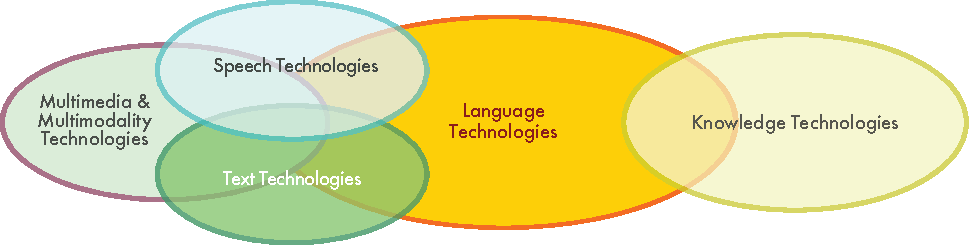
\includegraphics[width=\textwidth]{../_media/english/language_technologies}
  \caption{Language technologies}
  \label{fig:ltincontext_en}
  \colorrule{grey3}{\textwidth}{1.5pt}
\end{figure*}

\subsection{Application Architectures}

Software applications for language processing typically consist of several components that mirror different aspects of language. While such applications tend to be very complex, figure~\ref{fig:textprocessingarch_en} shows a highly simplified architecture of a typical text processing system. The first three modules handle the structure and meaning of the text input:

\begin{enumerate}
\item Pre-processing: cleans the data, analyses or removes formatting, detects the input languages, and so on.
\item Grammatical analysis: finds the verb, its objects, modifiers and other sentence elements; detects the sentence structure.
\item Semantic analysis: performs disambiguation (i.\,e., computes the appropriate meaning of words in a given context); resolves anaphora (i.\,e., which pronouns refer to which nouns in the sentence); represents the meaning of the sentence in a machine-readable way.
\end{enumerate}

After analysing the text, task-specific modules can perform other operations, such as automatic summarisation and database look-ups.

In the remainder of this section, we firstly introduce the core application areas for language technology, and follow this with a brief overview of the state of LT research and education today, and a description of past and present research programmes. Finally, we present an expert estimate of core LT tools and resources for Basque in terms of various dimensions such as availability, maturity and quality. 
The general situation of LT for the Basque language is summarised in
figure~\ref{fig:lrlttable_baen} (p.~\pageref{fig:lrlttable_baen}) at the end of this chapter. This table lists all tools and
resources that are boldfaced in the text.
LT support for Basque is also compared to other languages that are part of this series.


%    Typical software applications for language processing consist of several components that mirror different aspects of language and of the task they implement. Figure ~\ref{fig:textprocessingarch_en} displays a highly simplified architecture that can be found in a text processing system. The first three modules deal with the structure and meaning of the text input:
%    \begin{itemize}
%      \item Pre-processing: cleaning up the data, removing formatting, detecting the input language, etc. 
%      \item Grammatical analysis: finding the verb, its objects, modifiers and other sentence element; detecting the sentence structure.
%      \item Semantic analysis: disambiguation (Which meaning of “apple” is the right one in the given context?), resolving anaphora and referring expressions like “she”, “the car”, etc.; representing the meaning of the sentence in a machine-readable way.
%\end{itemize}

\begin{figure*}[b]
  \colorrule{grey3}{\textwidth}{1.5pt}
  \center
  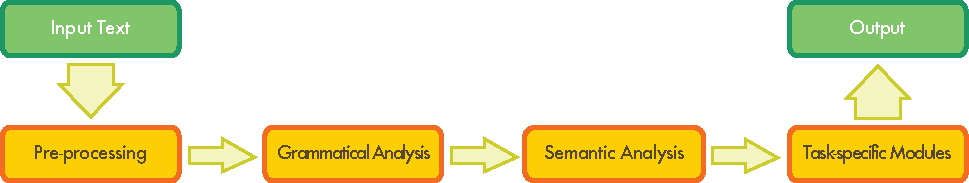
\includegraphics[width=\textwidth]{../_media/english/text_processing_app_architecture}
  \caption{A typical text processing architecture}
  \label{fig:textprocessingarch_en}
  \colorrule{grey3}{\textwidth}{1.5pt}
\end{figure*}
   
% Task-specific modules then perform many different operations such as automatic summarisation of an input text, database lookups and many others. Below, we will illustrate core application areas and highlight their core modules. Again, the architectures of the applications are highly simplified and idealised, to illustrate the complexity of Language Technology (LT) applications in a generally understandable way. The most important tools and resources involved are underlined in the text and can also be found in the table at the end of the chapter.  The sections discussing the core application areas also contain an overview of the industries active in the respective field in Basque.

%After introducing the core application areas, we will give a short overview of the situation in LT research and education, concluding with an overview of past and ongoing research programs. At the end of this section, we will present an expert estimation on the situation regarding core LT tools and resources on a number of dimensions such as availability, maturity, or quality. This table gives a good overview on the situation of LT for Basque.

\subsection{Core Application Areas}

    In this section, we focus on the most important LT tools and resources, and give an overview of LT activities in Basque. Tools and resources that are set in bold in the text can also be found in the table at the end of this chapter.

\subsubsection{Language Checking}
    Anyone using a word processing tool such as Microsoft Word has come across a 
%\textbf{spell checking} 
spell checking component that indicates spelling mistakes and proposes corrections. Forty years after the first spelling correction program by Ralph Gorin, language checkers nowadays do not simply compare the list of extracted words against a dictionary of correctly spelled words, but have become increasingly sophisticated. 
Using language-dependent algorithms for \textbf{grammatical analysis}, they detect errors related to morphology (e.\,g., plural formation) as well as syntax–related errors, such as a missing verb or a conflict of verb-subject agreement (e.\,g., \textit{she *write a letter}). However, most spell checkers will not find any errors in the following text \cite{zar1}:
%In addition to language-dependent algorithms for handling 
%\textbf{morphology} (e.g. plural formation), some are now capable of recognising syntax–related errors, such as a missing verb or a verb that does not agree with %its subject in person and number, e.g. in ‘She *write a letter.’ However, most available spell checkers (including Microsoft Word) will find no errors in the %following first verse of a poem by Jerrold H. Zar (1992):
 
\hspace{10pt}\textit{Eye have a spelling chequer,}

\hspace{10pt}\textit{It came with my Pea Sea.}

\hspace{10pt}\textit{It plane lee marks four my revue}

\hspace{10pt}\textit{Miss Steaks I can knot sea.}

For handling this type of errors, analysis of the 
%\textbf{context} 
context is needed in many cases, e.g., in Basque, for deciding if the ergative marker has to be used, as in:

\hspace{10pt}\textit{Liburua neskak dauka }

\hspace{10pt}\textit{[The girl has the book]}

\hspace{10pt}\textit{Irakurlea neska da.}

\hspace{10pt}\textit{[The reader is a girl.] }

\begin{figure*}[htb]
  \colorrule{grey3}{\textwidth}{1.5pt}
  \center
  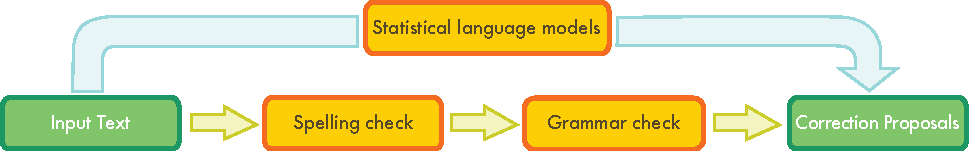
\includegraphics[width=\textwidth]{../_media/english/language_checking}
  \caption{Language checking (top: statistical; bottom: rule-based)}
  \label{fig:langcheckingaarch_en}
  \colorrule{grey3}{\textwidth}{1.5pt}
\end{figure*}

Language checking(see figure~\ref{fig:langcheckingaarch_en}) either requires the formulation of language-specific 
\textbf{grammars}, i.e. a high degree of expertise and manual labour, or the use of a so-called statistical 
%\textbf{language model}
language model.  Such models calculate the probability of a particular word occurring in a specific environment (i.e., the preceding and following words). For example, \textit{neskak dauka} is a much more probable word sequence than \textit{neska dauka}. A statistical language model can be automatically derived using a large amount of (correct) language data (i.e. a 
%\textbf{corpus})
corpus. Up to now, these approaches have mostly been developed and evaluated on English language data. However, they do not necessarily transfer straightforwardly to Basque with its richer inflection and agglutinative morphology. In fact, language modelling for Basque poses enormous difficulties due to the impossibility of collecting all possible word-forms.  

The use of Language Checking is not limited to word processing tools, but it is also applied in authoring support systems. Accompanying the rising number of technical products, the amount of technical documentation has rapidly increased over the last decades. Fearing customer complaints about wrong usage and damage claims resulting from bad or badly understood instructions, companies have begun to focus increasingly on the quality of technical documentation, and at the same time targeting the international market. Advances in natural language processing lead to the development of authoring support software, which assists the writer of technical documentation to use vocabulary and sentence structures consistent with certain rules and (corporate) terminology restrictions. 

\boxtext{Language checking is not limited to word processors but also applies to authoring systems}

The most used Spell Checker for Basque is the so-called ‘Xuxen \cite{BAS-Nota24}’, which was developed by the university research group IXA (ixa.si.ehu.es) and is supplied by the SME ‘Eleka Ingenieritza Linguistikoa’. This Spell Checker is not limited to the use of a lexicon as it is common practice for English or other less-inflected languages. On the contrary, morphological analysis is performed. The newest version of this spell checker also performs grammar and style corrections. This version also includes code developed by the company ‘Hizkia’ \cite{BAS-Nota25} and the institution ‘UZEI’ \cite{BAS-Nota26}. 

Besides spell checkers and authoring support, Language Checking is also important in the field of computer-assisted language learning and is applied to automatically correct queries sent to Web Search engines, e.g. Google’s ‘Did you mean…’ suggestions. 

\subsubsection{Web Search}
\begin{figure*}[htb]
  \colorrule{grey3}{\textwidth}{1.5pt}
  \center
  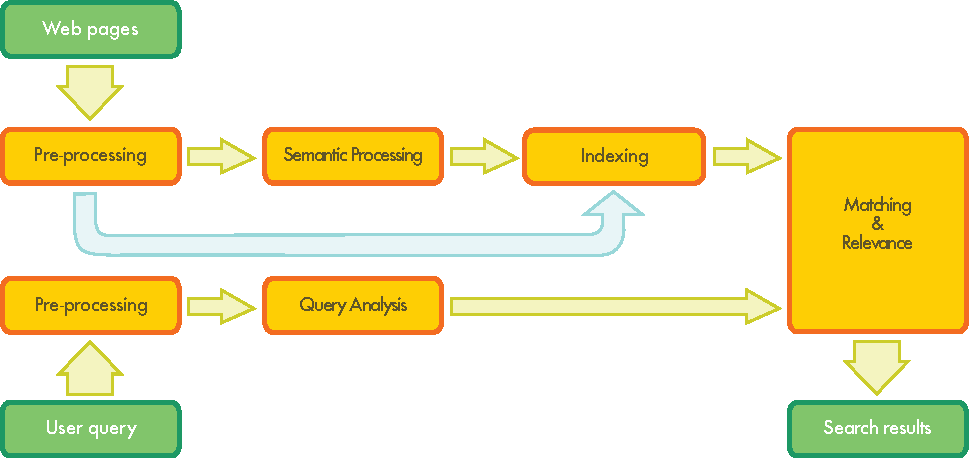
\includegraphics[width=\textwidth]{../_media/english/web_search_architecture}
  \caption{Web search architecture}
  \label{fig:websearcharch_en}
  \colorrule{grey3}{\textwidth}{1.5pt}
 \end{figure*}
 
    Search on the web, in intranets or in digital libraries, is probably the most widely used and yet underdeveloped Language Technology today. The search engine Google, which started in 1998, is nowadays used for about 80\% of all search queries world-wide \cite{BAS-Nota27}.
 
Neither the search interface nor the presentation of the retrieved results has significantly changed since the first version. In the current version, Google offers a spelling correction for misspelled words and also, in 2009, they incorporated basic semantic search capabilities into their algorithmic mix \cite{BAS-Nota28}, which can improve search accuracy by analysing the meaning of the query terms in context. The success story of Google shows that with a lot of data at hand and efficient techniques for indexing these data, a mainly statistically-based approach can lead to satisfactory results.
 
%However, for a more sophisticated request for information, integrating deeper linguistic knowledge is essential. In the research labs, experiments using %machine-readable thesauri and ontological language resources like WordNet have shown improvements by allowing the possibility of finding a page on the %basis of synonyms of the search terms. Again, these developments require of language specific resources. A Basque WordNet ‘BasWN’ has been developed %by the research group IXA at the University of the Basque Country and is commercially available through ELRA. 

%NEW!
For more sophisticated information requests, it is essential to integrate deeper linguistic knowledge to facilitate text interpretation. Experiments using \textbf{lexical resources} such as machine-readable thesauri or ontological language resources like WordNet have demonstrated improvements in finding pages using synonyms of the search terms. Again, these developments require language-specific resources. A Basque WordNet ‘BasWN’ has been developed by the research group IXA at the University of the Basque Country and is commercially available through ELRA. 

\boxtext{The next generation of search engines\\ will have to include much more sophisticated language technology}

%The next generation of search engines will have to include much more sophisticated Language Technology. If a search query consists of a question or %another type of sentence rather than a list of keywords, retrieving relevant answers to this query requires an analysis of this sentence on a syntactic and %semantic level as well as the availability of an index that allows for a fast retrieval of the relevant documents. 

The next generation of search engines will have to include much more sophisticated language technology, especially to deal with search queries consisting of a question or other sentence type rather than a list of keywords. For the query, \textit{Give me a list of all companies that were taken over by other companies in the last five years}, a syntactic as well as \textbf{semantic analysis} is required. The system also needs to provide an index to quickly retrieve relevant documents. A satisfactory answer will require syntactic parsing to analyse the grammatical structure of the sentence and determine that the user wants companies that have been acquired, rather than companies that have acquired other companies. 

%For example, imagine a user inputs the query ‘Give me a list of all companies that were taken over by other companies in the last five years’. For a %satisfactory answer, syntactic \textbf{parsing}  needs to be applied to analyse the grammatical structure of the sentence and determine that the user is %looking for companies that have been taken over and not companies that took over others. Also, the expression \textit{last five years} needs to be %processed in order to find out which years it refers to. For the expression \textit{last five years}, the system needs to determine the relevant range of years, taking into account the present year.

Finally, the processed query needs to be matched against a huge amount of unstructured data in order to find the piece or pieces of information the user is looking for. This is commonly referred to as 
%\textbf{information retrieval}
information retrieval and involves the search for and ranking of relevant documents. In addition, generating a list of companies, we also need to extract the information that a particular string of words in a document refers to a company name. This kind of information is made available by so-called 
%\textbf{named-entity recognisers}
named-entity recognisers. 

Even more demanding is the attempt to match a query to documents written in a different language. For 
%\textbf{cross-lingual information retrieval}
cross-lingual information retrieval, we have to automatically translate the query to all possible source languages and transfer the retrieved information back to the target language. The increasing percentage of data available in non-textual formats drives the demand for services enabling 
%\textbf{multimedia information retrieval}
multimedia information retrieval, i.e., information search on images, audio, and video data. For audio and video files, this involves a \textbf{speech recognition} module to convert speech content into text or a phonetic representation, to which user queries can be matched.

Focus on development for these companies lies on providing add-ons and advanced search engines for special-interest portals by exploiting topic-relevant semantics. Due to the still high demands in processing power, such search engines are only economically usable on relatively small \textbf{text corpora}. Processing time easily exceeds that of a common statistical search engine as, e.g., provided by Google by a magnitude of thousands. These search engines also have high demand in topic-specific domain modelling, making it not feasible to use these mechanisms on web scale.

In the Basque Autonomous Community, the small company ‘Eleka Ingeniaritza Linguistikoa’ has been very active in the development of applications and web based services for Basque. They usually integrate LT research results and resources such as lemmatisers and lexical databases of the IXA group and Elhuyar Foundation. The multilingual search engine \textit{elebila} considers the Basque language specifics and integrates various linguistic tools and resources to offer high quality search results for Basque. Another example is the tool called Miatu (‘Examine’ in Basque), a library offering functionality to search in special purpose indexed databases using lemmatisers and other morphology analysis tools. It has been used to develop the science related web portal www.zientzia.net and the educational content portal www.ikasbil.net.

\subsubsection{Speech Interaction}
\begin{figure*}[htb]
  \colorrule{grey3}{\textwidth}{1.5pt}
  \center
  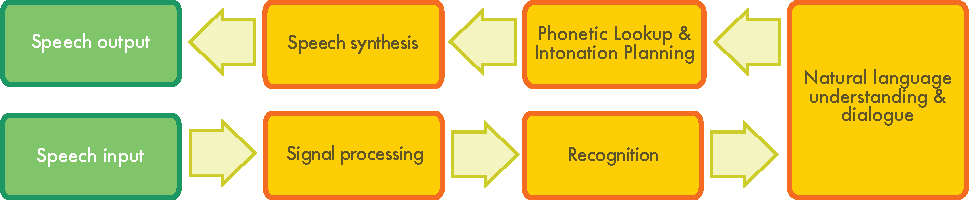
\includegraphics[width=\textwidth]{../_media/english/simple_speech-based_dialogue_architecture}
  \caption{Speech-based dialogue system}
  \label{fig:dialoguearch_en}
  \colorrule{grey3}{\textwidth}{1.5pt}
\end{figure*}

Speech Interaction technology is the basis for the creation of interfaces that allow a user to interact with machines using spoken language rather than, e.g., a graphical display, a keyboard, and a mouse. Today, such voice user interfaces (VUIs) are usually employed for partially or fully automating service offerings provided by companies to their customers, employees, or partners via the telephone. Business domains that rely heavily on VUIs are banking, logistics, public transportation, and telecommunications. Other usages of Speech Interaction technology are interfaces to particular devices, e.g. in-car navigation systems, and the employment of spoken language as an alternative to the input/output modalities of graphical user interfaces, e.g. in smartphones.

At its core, Speech Interaction comprises the following four differrent technologies:

    \begin{itemize}
      \item Automatic \textbf{speech recognition} (ASR) is responsible for determining which words were actually spoken given a sequence of sounds uttered by a user.
      \item Syntactic analysis and 
%\textbf{semantic interpretation} 
semantic interpretation deal with analysing the syntactic structure of a user’s utterance and interpretting the latter according to the purpose of the respective system.
      \item Dialogue management is required for determining, on the part of the system the user interacts with, which action shall be taken given the user’s input and the functionality of the system.
      \item \textbf{Speech synthesis} (Text-to-Speech, TTS) technology is employed for transforming the wording of that utterance into sounds that will be output to the user. 

    \end{itemize}

%One of the major challenges is to have an ASR system recognise the words uttered by a user as precisely as possible. This requires either a restriction of %the range of possible user utterances to a limited set of keywords, or the manual creation of 
%\textbf{language models} 
%language models that cover a large range of natural language user utterances. Whereas the former results in a rather rigid and inflexible usage of a VUI %and possibly causes a poor user acceptance, the creation, tuning and maintenance of language models may increase the costs significantly. However, VUIs %that employ language models and initially allow a user to flexibly express their intent – evoked, e.g., by a ‘How may I help you’ greeting – show both a %higher automation rate and a higher user acceptance and may therefore be considered as advantageous over a less flexible directed dialogue approach.

%NEW!
One of the major challenges of ASR systems is to accurately recognise the words a user utters. This means restricting the range of possible user utterances to a limited set of keywords, or manually creating language models that cover a large range of natural language utterances. Using machine learning techniques, language models can also be generated automatically from \textbf{speech corpora}, i.\,e., large collections of speech audio files and text transcriptions. Restricting utterances usually forces people to use the voice user interface in a rigid way and can damage user acceptance; but the creation, tuning and maintenance of rich language models will significantly increase costs. VUIs that employ language models and initially allow a user to express their intent more flexibly -- prompted by a \textit{How may I help you?} greeting -- are better accepted by users.

\boxtext{Speech interaction is the basis for interfaces that allow a user to interact with spoken language}

For the output part of a VUI, companies tend to use utterances pre-recorded by professional – ideally corporate – speakers a lot. For static utterances, in which the wording does not depend on the particular contexts of use or the personal data of the given user, this will result in a rich user experience. However, the more dynamic content an utterance needs to consider, the more the user experience may suffer from a poor prosody resulting from concatenating different parts of audio files. In contrast, today’s TTS systems prove superior, though optimisable, regarding the prosodic naturalness of dynamic utterances.  

Regarding the market for Speech Interaction technology, the last decade underwent a strong standardisation of the interfaces between the different technology components, as well as by standards for creating particular software artefacts for a given application. There also has been strong market consolidation within the last ten years, particularly in the field of ASR and TTS. Here, the national markets in the G20 countries – i.e. economically strong countries with a considerable population - are dominated by less than 5 players worldwide, with Nuance and Loquendo being the most prominent ones in Europe. Since 2007, thanks to the support given by the Basque Government, Basque language is included in the catalogue of products of Nuance. However, the offer in ASR is limited to small to medium size vocabulary applications and no dictation product is available. For TTS, just one female voice is available. On the Spanish market, the Catalan SME Verbio Speech Technologies \cite{BAS-Nota29}  also offers Basque both for ASR and TTS, with more than one voice.  Still, no commercial dictation system exists for Basque. 

Regarding dialogue management technology and know-how, mar-kets are strongly dominated by national players, which are usually SMEs. Most of the companies on the Spanish TTS market are essentially application developers. Key players in the Spanish market are: Indsys \cite{BAS-Nota30}  (Intelligent Dialogue Systems), Fonetic \cite{BAS-Nota31}, Ydilo \cite{BAS-Nota32}  and NaturalVox \cite{BAS-Nota33}. Some of them have a limited offer in Basque. Free TTS software for the Basque language is also offered by the research group Aholab \cite{BAS-Nota34} of the University of the Basque Country (UPV/EHU).

Looking beyond today’s state of technology, there will be significant changes due to the spread of smart phones as a new platform for managing customer relationships – in addition to the telephone, Internet, and email channels. This tendency will also affect the employment of technology for speech interaction. On one hand, demand for telephony-based VUIs will decrease, in the long run. On the other hand, the usage of spoken language as a user-friendly input modality for smart phones will gain significant importance. This tendency is supported by the observable improvement of speaker independent speech recognition accuracy for speech dictation services that are already offered as centralised services to smart phone users. Given this ‘outsourcing’ of the recognition task to the infrastructure of applications, the application-specific employment of linguistic core technologies will supposedly gain importance compared to the present situation. 

\subsubsection{Machine Translation}
    The idea of using digital computers for translation of natural languages came up in 1946 by A. D. Booth and was followed by substantial funding for research in this area in the 1950s and beginning again in the 1980s. Nevertheless, \textbf{Machine Translation} (MT) still fails to fulfil the high expectations it gave rise to in its early years. 
    
\boxtext{At its basic level, Machine Translation simply substitutes words in one natural language with words in another language}

\begin{figure*}[htb]
  \colorrule{grey3}{\textwidth}{1.5pt}
  \center
  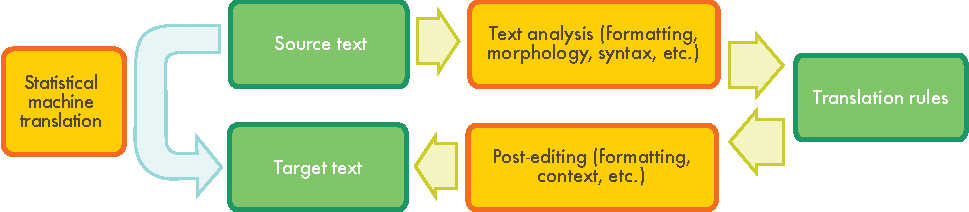
\includegraphics[width=\textwidth]{../_media/english/machine_translation}
  \caption{Machine translation (left: statistical; right: rule-based)}
  \label{fig:mtarch_en}
  \colorrule{grey3}{\textwidth}{1.5pt}
\end{figure*}

At its basic level, MT simply substitutes words in one natural language by words in another. This can be useful in subject domains with a very restricted, formulaic language, e.g., weather reports. However, for a good translation of less standardised texts, larger text units (phrases, sentences, or even whole passages) need to be matched to their closest counterparts in the target language. The major difficulty here lies in the fact that human language is ambiguous, which yields challenges on multiple levels, e.g., 
%\textbf{word sense disambiguation} 
word sense disambiguation at the lexical level (‘Jaguar’ can mean a car or an animal) or on other levels as in:

\textit{Egon garenetan ez dugu topatu}

\textit{[Each time we were there we have not seen him/her] or }

\textit{[In every place we were we have not seen him/her]}

\textit{Aitak semeari bere bizikleta eman dio}

\textit{[The father has given his bicycle to his son]}

One way of approaching the task is based on linguistic rules. For translations between closely related languages, a direct translation may be feasible in cases like in the second example above. But often rule-based (or knowledge-driven) systems analyse the input text and create an intermediary, symbolic representation, from which the text in the target language is generated. The success of these methods is highly dependent on the availability of extensive lexicons with morphological, syntactic, and semantic information, and large sets of grammar rules carefully designed by a skilled linguist.

Beginning in the late 1980s, as computational power increased and became less expensive, more interest was shown in statistical models for MT. The parameters of these statistical models are derived from the analysis of bilingual text 
%\textbf{corpora}
corpora, such as the Europarl 
\textbf{parallel corpus}, which contains the proceedings of the European Parliament in 21 European languages. Given enough data, statistical MT works well enough to derive an approximate meaning of a foreign language text. However, unlike knowledge-driven systems, statistical (or data-driven) MT often generates ungrammatical output. On the other hand, besides the advantage that less human effort is required for grammar writing, data-driven MT can also cover particularities of the language that go missing in knowledge-driven systems, for example idiomatic expressions. 

As the strengths and weaknesses of knowledge- and data-driven MT are complementary, researchers nowadays unanimously target hybrid approaches combining methodologies of both. This can be done in several ways. One is to use both knowledge- and data-driven systems and have a selection module decide on the best output for each sentence. However, for longer sentences, no result will be perfect. A better solution is to combine the best parts of each sentence from multiple outputs, which can be fairly complex, as corresponding parts of multiple alternatives are not always obvious and need to be aligned. 

For Basque, MT is particularly challenging. The rich morphology, the high degree of inflection and the agglutinative character of the language makes dictionary analysis and dictionary coverage difficult. Additionally, due to the order of the sentence components, \textbf{parallel corpora} are difficult to manage. 

\textit{Matxin} is a Transfer-based MT system from Spanish into Basque developed by IXA Group at the University of the Basque Country (UPV/EHU). It is an open, reusable and interoperable framework useful even for other language-pairs (matxin.sourceforge.org). It uses other open source codes such as Freeling, and reuses Basque morphology for morphological generation. IXA Group has also created an improved Statistical Machine Translation system for Basque Spanish that deals with morphological segmentation and word reordering (EUSMT. \url{http://ixa2.si.ehu.es/openmt-demo/}).  For the development of these MT systems, there is strong collaboration between the university research group, the local SME \textit{Eleka Ingeniaritza Linguistikoa} and the \textit{Elhuyar Foundation}, which provides considerable amounts of linguistic resources. This SME has also developped the translator Standard Basque \textit{batua} - Western dialect \textit{bizkaiera}. Also, a Basque to Spanish initial system has been developed by the Transducens Group at Universitat d’Alacant, using the platform Apertium.  Google's Translator offers an alpha version for Basque.

Leading international MT developer Lucy Software has an important subsidiary in Spain, Lucy Iberica \cite{BAS-Nota35}, former Trans\-len\-dium. This company was selected in 2008 by the Basque Government to develop a Spanish-Basque translation system and again in 2011 to continue the work. 

Provided good adaptation in terms of user-specific terminology and workflow integration, there is a wide consensus that the use of MT can increase productivity significantly. The quality of MT systems is still considered to have huge improvement potential. Challenges include the adaptability of the language resources to a given subject domain or user area and the integration into existing workflows with term bases and translation memories. In addition, many language pairs are still missing.

%NEW!
Evaluation campaigns help to compare the quality of MT systems, their approaches and the status of the systems for different language pairs. Figure~\ref{fig:euromatrix_de} (p.~\pageref{fig:euromatrix_de}), which was prepared during the Euromatrix+ project, shows the pair-wise performances obtained for 22 of the 23 EU languages (Irish was not compared). The results are ranked according to a BLEU score, which indicates higher scores for better translations \cite{bleu1}. A human translator would normally achieve around 80 points. The best results (in green and blue) were achieved by languages that benefit from a considerable research effort in coordinated programmes and the existence of many parallel corpora (e.\,g., English, French, Dutch, Spanish and German). The languages with poorer results are shown in red. These either lack such development efforts or are structurally very different from other languages (e.\,g., Hungarian, Maltese, Finnish).

\subsection{Other Application Areas}
    Building Language Technology applications involves a range of subtasks that do not always surface at the level of interaction with the user,  but provide significant service functionalities ‘under the hood’ of the system. Therefore, they constitute important research issues that have become individual sub-disciplines of Computational Linguistics in academia. 

Question answering has become an active area of research, for which annotated corpora have been built and scientific competitions have been started. The idea is to move from keyword-based search (to which the engine responds with a whole collection of potentially relevant documents) to the scenario of the user asking a concrete question and the system providing a single answer. For example:

\begin{itemize}
\item[] \textit{Question: How old was Neil Armstrong when he stepped on the moon?}
\item[] \textit{Answer: 38.}
\end{itemize}

While this is obviously related to the aforementioned core area Web Search, question answering nowadays is primarily an umbrella term for research questions such as what \textit{types} of questions should be distinguished and how should they be handled, how can a set of documents that potentially contain the answer be analysed and compared (do they give conflicting answers?), and how can specific information - the answer - be reliably extracted from a document, without unduly ignoring the context. 

\boxtext{Language technology applications often provide significant service functionalities behind the scenes of larger software systems}

This is in turn related to the information extraction (IE) task, an area that was extremely popular and influential at the time of the ‘statistical turn’ in Computational Linguistics, in the early 1990s. IE aims at identifying specific pieces of information in specific classes of documents; this could e.g. be the detection of the key players in company takeovers as reported in newspaper stories. Another scenario that has been worked on is reports on terrorist incidents, where the problem is to map the text to a template specifying the perpetrator, the target, time and location of the incident, and the results of the incident. Domain-specific template-filling is the central characteristic of IE, which for this reason is another example of a ‘behind the scenes’ technology that constitutes a well-demarcated research area but for practical purposes then needs to be embedded into a suitable application environment. 

Two ‘borderline’ areas, which sometimes play the role of stand-alone application and sometimes that of supportive, ‘under the hood’ component are %\textbf{text summariza\-tion} 
text summariza\-tion and \textbf{text generation}. Summarisation, obviously, refers to the task of making a long text short, and is offered for instance as a functionality within MS Word. It works largely on a statistical basis, by first identifying ‘important’ words in a text (that is, for example, words that are highly frequent in this text but markedly less frequent in general language use) and then determining those sentences that contain many important words. These sentences are then marked in the document, or extracted from it, and are taken to constitute the summary. In this scenario, which is by far the most popular one, summarisation equals sentence extraction: the text is reduced to a subset of its sentences. All commercial summarisers make use of this idea. An alternative approach, to which some research is devoted, is to actually synthesise \textit{new sentences}, i.e., to build a summary of sentences that need not show up in that form in the source text. This requires a certain amount of deeper understanding of the text and therefore is much less robust. All in all, a text generator is in most cases not a stand-alone application but embedded into a larger software environment, such as into the clinical information system where patient data is collected, stored and processed, and report generation is just one of many functionalities.

\boxtext{For Basque and for most languages, research in most text technologies is much less developed than for English}

For Basque, the situation in all these research areas is much less developed than it is for English, where question answering, information extraction, and summarisation have since the 1990s been the subject of numerous open competitions, primarily those organised by DARPA/NIST in the United States. These have significantly improved the state of the art, but the focus has always been on English; some competitions have added multilingual tracks, but Basque was never a targeted language. Accordingly, there are hardly available annotated corpora or other resources for these tasks. Summarisation systems, when using purely statistical methods, are often to a good extent language-independent, and thus some research prototypes are available. For text generation, reusable components have traditionally been limited to the surface realisation modules (the "generation grammars"); again, most available software is for English.

\subsection{Language Technology in Education}
   Language Technology is a highly interdisciplinary field, involving the expertise of linguists, computer scientists, mathematicians, philosophers, psycholinguists, and neuroscientists, among others. Consequently, the current basic training of a computational linguist may be performed in Spain within the framework of a degree in Philology or Linguistics, which includes Computational Linguistics as a core subject, or by Computational Science faculties. Among the Universities that offer the first option: Universitat de Barcelona, Universitat Pompeu Fabra, Universitat Oberta de Catalunya and Universidade de Vigo. On the other hand, main computational science faculties offering Computational Linguistic as subject are: Universidad Politécnica de Madrid, Universidad Carlos III, Universidad Autónoma de Madrid, Universitat d’Alacant, Universidad Nacional de Educación a Distancia and Universidad del País Vasco / Euskal Herriko Unibertsitatea. Other cases, such as the Universidad Complutense combine both.

Graduate courses offer a more targeted professional training. There are several doctoral programs which offer masters or subjects related to language and speech processing. A complete doctoral program on Language Processing is offered by Universidad del País Vasco / Euskal Herriko Unibertsitatea, also totally offered in Basque. Modules in Language Technology are also offered to students of other master or PhD courses, particularly in Speech Processing (e.g. Master TICRM of the UPV/EHU). 

There are several research groups spread across the 3 universities of the Basque Autonomous Community, working on speech processing, speech synthesis and conversion, speech and speaker recognition, language recognition, natural language processing, text-to-text translation and speech-to-speech translation. All of them are members of the Sociedad Española para el Procesamiento del Lenguaje Natural (SEPLN, Spanish Society for Natural Language Processing), a non-profit organisation with over 300 members, both from academia and industry, which was created in 1984 with the purpose to promote and spread activities related to teaching, research and development of NLP, on both national and international level. SEPLN organises seminaries, symposiums and conferences and promotes collaboration with national and international institutions.

SEPLN organises an annual conference, which is attended yearly by an increasing number of researchers working on NLP, both from Spain and abroad. The association also edits a periodical journal and maintains a web server with information about issues related to the natural language processing and an open forum for members.

The Spanish Network on Speech Technology (RTTH) \cite{BAS-Nota36}  is a common forum where researchers (presently more than 25o researchers) in Speech Technology gather to combine efforts and share experiences in order to:
\begin{itemize}

       \item Promote research in speech technology to attract new young researchers in this field through training, student exchanges, scholarships and awards.
       
       \item Attract investments for business research by finding new applications that offer new business opportunities.  
      
      \item Progress in building partnerships and integration of network members to maintain Spain's leadership in the investigation of Spanish, and also enhance co-official languages such as Catalan, Euskara and Galician.

\end{itemize}

RTTH has been promoting every other year the “Jornadas en Tecnología del Habla” since 2000. This workshop pursues the aims of being a meeting point to present and discuss the results of the research on speech and language technologies on Iberian languages. They also aim at promoting industry/university collaboration. A wide variety of activities: technical papers presentations, keynote lectures, presentation of project reports and laboratories activities, demos, and recent PhD thesis presentations are defined.

\subsection{Language Technology Programs}
    Technology programs for the Basque language have been supported mainly by the Basque and the Spanish Government. 

The Spanish Ministries of Education and Science and Innovation have supported research in the field of information technologies through national research programs. These programs have impelled numerous research projects and collaboration with international research centres and companies. The basis of technology development and commercial applications for automated processing of the Basque language has been partly created as a result of these projects.

Since 2000 up till today, the Spanish Government supported within the National Plan of Research and Technology several projects in the area of Multilingual Speech Technologies: TEHAM, AVIVAVOZ, and BUCEADOR. Their main purpose was to improve the quality of Speech Recognition, Speech Translation and Text to Speech Synthesis in all the official languages spoken in Spain: Basque, Galician, Catalan and Spanish.

The Centre for the Development of Industrial Technology (CDTI) is a Spanish public organisation, under the Ministry of Science and Innovation, whose objective is to help Spanish companies to increase their technological profile. CDTI evaluates and finances R\&D projects through programmes such as CENIT (finalised in 2010) and AVANZA.

The Basque Government supports research and innovation through the “Plan de Ciencia y Tecnología” (PCTI). Within this plan, several bodies and research and innovation agencies have been created in the last years: \textit{The Basque Council for Science, Technology and Innovation} (the highest political body leading actions to promote and develop research and innovation), \textit{InnoBasque} (The Basque Agency for Innovation) and \textit{IkerBasque} (Basque Foundation for Science), whose main instrument is the attraction of talented researchers to the Basque Science and Technology system.  Important instruments of the PCTI plan are the calls for research and innovation projects: the program \textit{ETORTEK}, addressed to the agents of\textit{ Basque Network for Science, Technology and Innovation}, and the program \textit{ETORGAI}, addressed to private companies. 

In the last \textit{PCTI2010}, as had already been in previous plans, Language Tecnologies have been identified as one strategic field. As such, during the last 10 years, the projects \textit{HIZKING21, ANHITZ}, and presently \textit{BERBATEK} \cite{BAS-Nota37}  have been carried out under the \textit{ETORTEK} program. Most of the existing resources and tools for Basque have been obtained through these projects.
  
\subsection{Availability of Tools and Resources}

    Table ~\ref{fig:lrlttable_baen} provides an overview of the current situation of Language Technology support for Basque. Several leading experts rated the existing tools and resources based on educated estimations using seven criteria (each ranging from 0 to 6):

\begin{figure*}[htb]
\centering
%\begin{tabular}{>{\columncolor{orange1}}p{.33\linewidth}ccccccc} % ORIGINAL
\begin{tabular}{>{\columncolor{orange1}}p{.33\linewidth}@{\hspace*{6mm}}c@{\hspace*{6mm}}c@{\hspace*{6mm}}c@{\hspace*{6mm}}c@{\hspace*{6mm}}c@{\hspace*{6mm}}c@{\hspace*{6mm}}c}
\rowcolor{orange1}
 \cellcolor{white}&\begin{sideways}\makecell[l]{Quantity}\end{sideways}
&\begin{sideways}\makecell[l]{\makecell[l]{Availability} }\end{sideways} &\begin{sideways}\makecell[l]{Quality}\end{sideways}
&\begin{sideways}\makecell[l]{Coverage}\end{sideways} &\begin{sideways}\makecell[l]{Maturity}\end{sideways} &\begin{sideways}\makecell[l]{Sustainability}\end{sideways} &\begin{sideways}\makecell[l]{Adaptability}\end{sideways} \\ \addlinespace
\multicolumn{8}{>{\columncolor{orange2}}l}{Language Technology: Tools, Technologies and Applications} \\ \addlinespace

Speech Recognition &2&1&1&1&4&3&2 \\ \addlinespace
Speech Synthesis &2&3&4&4&4&3&3 \\ \addlinespace
Grammatical analysis &4&2.5&4&4&4&2.5&2.5 \\ \addlinespace
Semantic analysis &1&1.5&2&1&1&1&1\\ \addlinespace
Text generation &1&0&0&0&0&0&0\\ \addlinespace
Machine translation &3&5&2&3&3&2&2\\ \addlinespace

\multicolumn{8}{>{\columncolor{orange2}}l}{\textcolor{black}{Language Resources (Resources, Data and Knowledge Bases)}} \\ \addlinespace

Text corpora &2&4&3&2&3&4&2.5\\ \addlinespace
Speech corpora &3&2&3&2&3&3&2\\ \addlinespace
Parallel corpora &2&4&2&2&2&2&1\\ \addlinespace
Lexical resources &4&4&4&5&5&4&3\\ \addlinespace
Grammars &2&2&2&2&2&2&2\\

\end{tabular}
\caption{State of language technology support for Basque}
\label{fig:lrlttable_baen}
\end{figure*}

    In this White Paper Series, a first effort has been made to assess the overall situation of many European languages with respect to language technology support in a way that allows for high level comparison and identification of gaps and needs.

For Basque, key results regarding technologies and resources include the following:

    \begin{itemize}
      \item Speech processing developments currently show a more mature situation for speech synthesis than for speech recognition. More efforts have to be done in the development of language models that account for the special morphology of Basque.   
      \item Everyday applications that integrate speech technology such as voice-based interfaces to mobile phones, car navigation systems or spoken dialog systems are rarely available in Basque. 
      \item The spelling checker is one of the most powerful tools in the ongoing standardisation of Basque and the most representative of the effective LT tools created to promote the use of Basque. 
      \item Standard resources for Basque have adopted TEI and XML standards as a basis for linguistic annotation at the different levels of processing, and also to the definition of a general methodology for written corpus annotation. However, several resources lack standardisation, i.e., even if they exist, sustainability is not always given; concerted programs and initiatives are needed to standardise data and interchange formats.
      \item Text semantics is more difficult to process than word and sentence semantics. There is a Wordnet for Basque, and promising algorithms to examine similarity between words and to extract facts from text have been developed. 
    \end{itemize}
    
    From this, it is clear that more efforts need to be directed into the creation of resources for Basque and into research, innovation, and development. The need for large amounts of data and the high complexity of language technology systems make it also mandatory to develop new infrastructures for sharing and cooperation.

\subsection{Cross-language comparison}

\begin{figure*}[tb]
  \small
  \centering
  \begin{tabular}
  { % defines color for each column.
  >{\columncolor{corange5}}p{.13\linewidth}@{\hspace{.040\linewidth}}
  >{\columncolor{corange4}}p{.13\linewidth}@{\hspace{.040\linewidth}}
  >{\columncolor{corange3}}p{.13\linewidth}@{\hspace{.040\linewidth}}
  >{\columncolor{corange2}}p{.13\linewidth}@{\hspace{.040\linewidth}}
  >{\columncolor{corange1}}p{.13\linewidth} 
  }
  \multicolumn{1}{>{\columncolor{white}}c@{\hspace{.040\linewidth}}}{\textbf{Excellent}} & 
  \multicolumn{1}{@{}>{\columncolor{white}}c@{\hspace{.040\linewidth}}}{\textbf{Good}} &
  \multicolumn{1}{@{}>{\columncolor{white}}c@{\hspace{.040\linewidth}}}{\textbf{Moderate}} &
  \multicolumn{1}{@{}>{\columncolor{white}}c@{\hspace{.040\linewidth}}}{\textbf{Fragmentary}} &
  \multicolumn{1}{@{}>{\columncolor{white}}c}{\textbf{Weak/no}} \\ 
  \multicolumn{1}{>{\columncolor{white}}c@{\hspace{.040\linewidth}}}{\textbf{support}} & 
  \multicolumn{1}{@{}>{\columncolor{white}}c@{\hspace{.040\linewidth}}}{\textbf{support}} &
  \multicolumn{1}{@{}>{\columncolor{white}}c@{\hspace{.040\linewidth}}}{\textbf{support}} &
  \multicolumn{1}{@{}>{\columncolor{white}}c@{\hspace{.040\linewidth}}}{\textbf{support}} &
  \multicolumn{1}{@{}>{\columncolor{white}}c}{\textbf{support}} \\ \addlinespace
  
& \vspace*{0.5mm}English
& \vspace*{0.5mm}
Czech \newline 
Dutch \newline 
Finnish \newline 
French \newline 
German \newline   
Italian \newline  
Portuguese \newline 
Spanish \newline
& \vspace*{0.5mm}\textbf{Basque} \newline 
Bulgarian \newline 
Catalan \newline 
Danish \newline 
Estonian \newline 
Galician\newline 
Greek \newline  
Hungarian  \newline
Irish \newline  
Norwegian \newline 
Polish \newline 
Serbian \newline 
Slovak \newline 
Slovene \newline 
Swedish \newline
& \vspace*{0.5mm}
Croatian \newline 
Icelandic \newline  
Latvian \newline 
Lithuanian \newline 
Maltese \newline 
Romanian\\
\end{tabular}
\caption{Speech processing: state of language technology support for 30 European languages}
\label{fig:speech_cluster_en}
\end{figure*}

\begin{figure*}[tb]
  \small
  \centering
  \begin{tabular}
  { % defines color for each column.
  >{\columncolor{corange5}}p{.13\linewidth}@{\hspace{.040\linewidth}}
  >{\columncolor{corange4}}p{.13\linewidth}@{\hspace{.040\linewidth}}
  >{\columncolor{corange3}}p{.13\linewidth}@{\hspace{.040\linewidth}}
  >{\columncolor{corange2}}p{.13\linewidth}@{\hspace{.040\linewidth}}
  >{\columncolor{corange1}}p{.13\linewidth} 
  }
  \multicolumn{1}{>{\columncolor{white}}c@{\hspace{.040\linewidth}}}{\textbf{Excellent}} & 
  \multicolumn{1}{@{}>{\columncolor{white}}c@{\hspace{.040\linewidth}}}{\textbf{Good}} &
  \multicolumn{1}{@{}>{\columncolor{white}}c@{\hspace{.040\linewidth}}}{\textbf{Moderate}} &
  \multicolumn{1}{@{}>{\columncolor{white}}c@{\hspace{.040\linewidth}}}{\textbf{Fragmentary}} &
  \multicolumn{1}{@{}>{\columncolor{white}}c}{\textbf{Weak/no}} \\ 
  \multicolumn{1}{>{\columncolor{white}}c@{\hspace{.040\linewidth}}}{\textbf{support}} & 
  \multicolumn{1}{@{}>{\columncolor{white}}c@{\hspace{.040\linewidth}}}{\textbf{support}} &
  \multicolumn{1}{@{}>{\columncolor{white}}c@{\hspace{.040\linewidth}}}{\textbf{support}} &
  \multicolumn{1}{@{}>{\columncolor{white}}c@{\hspace{.040\linewidth}}}{\textbf{support}} &
  \multicolumn{1}{@{}>{\columncolor{white}}c}{\textbf{support}} \\ \addlinespace
  
& \vspace*{0.5mm} English 
& \vspace*{0.5mm} 
French \newline 
Spanish
& \vspace*{0.5mm}
Catalan \newline 
Dutch \newline 
German \newline 
Hungarian \newline
Italian \newline 
Polish \newline 
Romanian \newline 
& \vspace*{0.5mm}\textbf{Basque} \newline 
Bulgarian \newline 
Croatian \newline 
Czech \newline
Danish \newline 
Estonian \newline 
Finnish \newline 
Galician \newline 
Greek \newline 
Icelandic \newline 
Irish \newline 
Latvian \newline 
Lithuanian \newline 
Maltese \newline 
Norwegian \newline 
Portuguese \newline 
Serbian \newline 
Slovak \newline 
Slovene \newline 
Swedish \newline 
\end{tabular}
\caption{Machine translation: state of language technology support for 30 European languages}
\label{fig:mt_cluster_en}
\end{figure*}

\begin{figure*}[tb]
  \small
  \centering
  \begin{tabular}
  { % defines color for each column.
  >{\columncolor{corange5}}p{.13\linewidth}@{\hspace{.040\linewidth}}
  >{\columncolor{corange4}}p{.13\linewidth}@{\hspace{.040\linewidth}}
  >{\columncolor{corange3}}p{.13\linewidth}@{\hspace{.040\linewidth}}
  >{\columncolor{corange2}}p{.13\linewidth}@{\hspace{.040\linewidth}}
  >{\columncolor{corange1}}p{.13\linewidth} 
  }
  \multicolumn{1}{>{\columncolor{white}}c@{\hspace{.040\linewidth}}}{\textbf{Excellent}} & 
  \multicolumn{1}{@{}>{\columncolor{white}}c@{\hspace{.040\linewidth}}}{\textbf{Good}} &
  \multicolumn{1}{@{}>{\columncolor{white}}c@{\hspace{.040\linewidth}}}{\textbf{Moderate}} &
  \multicolumn{1}{@{}>{\columncolor{white}}c@{\hspace{.040\linewidth}}}{\textbf{Fragmentary}} &
  \multicolumn{1}{@{}>{\columncolor{white}}c}{\textbf{Weak/no}} \\ 
  \multicolumn{1}{>{\columncolor{white}}c@{\hspace{.040\linewidth}}}{\textbf{support}} & 
  \multicolumn{1}{@{}>{\columncolor{white}}c@{\hspace{.040\linewidth}}}{\textbf{support}} &
  \multicolumn{1}{@{}>{\columncolor{white}}c@{\hspace{.040\linewidth}}}{\textbf{support}} &
  \multicolumn{1}{@{}>{\columncolor{white}}c@{\hspace{.040\linewidth}}}{\textbf{support}} &
  \multicolumn{1}{@{}>{\columncolor{white}}c}{\textbf{support}} \\ \addlinespace

& \vspace*{0.5mm}English
& \vspace*{0.5mm}
  Dutch \newline 
  French \newline 
  German \newline 
  Italian \newline 
  Spanish
& \vspace*{0.5mm}\textbf{Basque} \newline 
  Bulgarian \newline 
  Catalan \newline 
  Czech \newline 
  Danish \newline 
  Finnish \newline 
  Galician \newline 
  Greek \newline 
  Hungarian \newline 
  Norwegian \newline 
  Polish \newline 
  Portuguese \newline 
  Romanian \newline 
  Slovak \newline 
  Slovene \newline 
  Swedish \newline 
& \vspace*{0.5mm}
  Croatian \newline 
  Estonian \newline 
  Icelandic \newline 
  Irish \newline 
  Latvian \newline 
  Lithuanian \newline 
  Maltese \newline 
  Serbian \\
  \end{tabular}
\caption{Text analysis: state of language technology support for 30 European languages}
\label{fig:text_cluster_en}
\end{figure*}

\begin{figure*}[tb]
  \small
  \centering
  \begin{tabular}
  { % defines color for each column.
  >{\columncolor{corange5}}p{.13\linewidth}@{\hspace{.040\linewidth}}
  >{\columncolor{corange4}}p{.13\linewidth}@{\hspace{.040\linewidth}}
  >{\columncolor{corange3}}p{.13\linewidth}@{\hspace{.040\linewidth}}
  >{\columncolor{corange2}}p{.13\linewidth}@{\hspace{.040\linewidth}}
  >{\columncolor{corange1}}p{.13\linewidth} 
  }
  \multicolumn{1}{>{\columncolor{white}}c@{\hspace{.040\linewidth}}}{\textbf{Excellent}} & 
  \multicolumn{1}{@{}>{\columncolor{white}}c@{\hspace{.040\linewidth}}}{\textbf{Good}} &
  \multicolumn{1}{@{}>{\columncolor{white}}c@{\hspace{.040\linewidth}}}{\textbf{Moderate}} &
  \multicolumn{1}{@{}>{\columncolor{white}}c@{\hspace{.040\linewidth}}}{\textbf{Fragmentary}} &
  \multicolumn{1}{@{}>{\columncolor{white}}c}{\textbf{Weak/no}} \\ 
  \multicolumn{1}{>{\columncolor{white}}c@{\hspace{.040\linewidth}}}{\textbf{support}} & 
  \multicolumn{1}{@{}>{\columncolor{white}}c@{\hspace{.040\linewidth}}}{\textbf{support}} &
  \multicolumn{1}{@{}>{\columncolor{white}}c@{\hspace{.040\linewidth}}}{\textbf{support}} &
  \multicolumn{1}{@{}>{\columncolor{white}}c@{\hspace{.040\linewidth}}}{\textbf{support}} &
  \multicolumn{1}{@{}>{\columncolor{white}}c}{\textbf{support}} \\ \addlinespace
    
& \vspace*{0.5mm}English
& \vspace*{0.5mm} 
    Czech \newline 
    Dutch \newline 
    French \newline 
    German \newline 
    Hungarian \newline
    Italian \newline
    Polish \newline
    Spanish \newline
    Swedish \newline 
& \vspace*{0.5mm} \textbf{Basque}\newline 
    Bulgarian\newline 
    Catalan \newline 
    Croatian \newline 
    Danish \newline 
    Estonian \newline 
    Finnish \newline 
    Galician \newline 
    Greek \newline 
    Norwegian \newline 
    Portuguese \newline 
    Romanian \newline 
    Serbian \newline 
    Slovak \newline 
    Slovene \newline
&  \vspace*{0.5mm}
    Icelandic \newline 
    Irish \newline 
    Latvian \newline 
    Lithuanian \newline 
    Maltese  \\
  \end{tabular}
  \caption{Speech and text resources: State of support for 30 European languages}  
  \label{fig:resources_cluster_en}
\end{figure*}

 The current state of LT support varies considerably from one language community to another. In order to compare the situation between languages, this section will present an evaluation based on two sample application areas (machine translation and speech processing) and one underlying technology (text analysis), as well as basic resources needed for building LT applications. The languages were clustered using the following five-point scale: 

\begin{enumerate}
\item Excellent support
\item Good support
\item Moderate support
\item Fragmentary support
\item Weak or no support
\end{enumerate}

LT support was measured according to the following criteria:\\
\textbf{Speech Processing:} Quality of existing speech recognition technologies, quality of existing speech synthesis technologies, coverage of domains, number and size of existing speech corpora, amount and variety of available speech-based applications.

\textbf{Machine Translation:} Quality of existing MT technologies, number of language pairs covered, coverage of linguistic phenomena and domains, quality and size of existing parallel corpora, amount and variety of available MT applications.

\textbf{Text Analysis:} Quality and coverage of existing text analysis technologies (morphology, syntax, semantics), coverage of linguistic phenomena and domains, amount and variety of available applications, quality and size of existing (annotated) text corpora, quality and coverage of existing lexical resources (e.g., WordNet) and grammars.

\textbf{Resources:} Quality and size of existing text corpora, speech corpora and parallel corpora, quality and coverage of existing lexical resources and grammars.

%\textit{Cluster description (for Text Analysis and Resources)}
%    \begin{itemize}
%      \item Cluster 1 (excellent LT support): Technologies/resources exist that are in widespread use and cover practically all linguistic phenomena (vocabulary, compounds, grammar, metaphors etc.) of a language.
%      \item Cluster 2 (very good support): Technologies/resources exist that are used in a variety of applications and cover the most important linguistic phenomena. 
%      \item Cluster 3 (good support): Technologies/resources exist that cover a reasonable amount of linguistic phenomena and are used in applications that are usually domain-specific.
%      \item Cluster 4 (medium support): Research prototypes/resources exist, but quality and coverage varies.
%      \item Cluster 5 (low to almost no support): From the drawing board to rudimentary prototypes (very limited quality and coverage, toy systems)
%    \end{itemize}
    
Figures~\ref{fig:speech_cluster_en} to~\ref{fig:resources_cluster_en} show that, thanks to LT funding programs from the Spanish and Basque governments in recent decades, the Basque language is equipped as most of other European languages. It compares well with languages spoken by a bigger number of speakers despite these are official languages of EU countries. This is mainly due to coordinated efforts of research groups and small developers of LT tools. But LT resources and tools for Basque clearly do not yet reach the quality, size and coverage of comparable resources and tools for the Spanish language, which is in a good position in almost all LT areas. There are still some gaps in Basque language resources and tools with regard to high quality applications. 

    For speech processing, current technologies perform well enough to be successfully integrated into a limited number of industrial applications such as IVR spoken dialogue systems, although there is still a gap to fill for dictation systems, even in a constrained domain. Machine Translation systems do not get a good performance yet, due to the fact that Basque is very different from the Indo-European languages. Deeper statistical classifiers are needed compared to other language pairs with similar origin, such as Catalan-Spanish or Galician-Spanish. There is a clear need for resources and technologies to cover a wider range of linguistic aspects and to allow a deep semantic analysis of the input text. By improving the quality and coverage of these basic resources and technologies, we shall be able to open up new opportunities for tackling a vast range of advanced application areas, including high-quality machine translation and continuous speech recognition.  

\subsection{Conclusions}

    \emph{In this series of white papers, we have made an important initial effort to assess language technology support for 30 European languages, and provide a high-level comparison across these languages. By identifying the gaps, needs and deficits, the European language technology community and related stakeholders are now in a position to design a large scale research and development programme aimed at building a truly multilingual, technology-enabled Europe.}

    We have seen that there are huge differences between Europe’s languages. While there are good quality software and resources available for some languages and application areas, others (usually “smaller” languages) have substantial gaps. Many languages lack basic technologies for text analysis and the essential resources for developing these technologies. Others have basic tools and resources but are as yet unable to invest in semantic processing. We therefore still need to make a large-scale effort to attain the ambitious goal of providing high-quality machine translation between all European languages.

   The situation of Basque concerning language technology support gives rise to cautious optimism. There is a viable LT research community in the Basque Country, which has been mainly supported by Spanish and Basque research programmes. A number of resources and state-of-the-art technologies have been produced and distributed for Basque. However, the scope of the resources and the range of tools are still very limited when compared to the resources and tools for the Spanish language (and obviously for the English language) and they are simply not sufficient in quality and quantity to develop the kind of technologies required to support a truly multilingual knowledge society.

    The Basque language technology industry is well established and a significant number of SME are active in this sector, although mostly for written technologies.  Their products have been and still are effective tools supporting the standardisation process and promoting the use of Basque.  Basque has not been included in the catalogue of large companies, except for a few specific actions, and usually supported by the Basque Government. 

There are several research groups working in speech and language processing since 1988. If Basque is now an exception to the correlation between language size and LR scarcity is due to the coordinated efforts of those research groups. Research and development for less resourced languages should be faced following high standardisation criteria, open-source coding and reusing   language foundations, tools and applications. 

    Our findings show that the only alternative is to make a substantial effort to create LT resources for Basque, and use them to drive forward research, innovation and development. The need for large amounts of data and the extreme complexity of language technology systems makes it vital to develop a new infrastructure and a more coherent research organisation to spur greater sharing and cooperation. Open source initiatives and the 2.0 communities can be important instruments for a rapid and sustainable development of tools and resources for less resourced languages.

   There is also a lack of continuity in research and development funding. Short-term coordinated programmes tend to alternate with periods of sparse or zero funding. In addition, there is an overall lack of coordination with programmes in other EU countries and at the European Commission level. We can therefore conclude that there is a desperate need for a large, coordinated initiative focused on overcoming the differences in language technology readiness for European languages as a whole.

    META-NET’s long-term goal is to introduce high-quality language technology for all languages in order to achieve political and economic unity through cultural diversity. The technology will help tear down existing barriers and build bridges between Europe’s languages. This requires all stakeholders - in politics, research, business, and society - to unite their efforts for the future. 
\end{multicols}

\clearpage


% --------------------------------------------------------------------------
\ssection[About META-NET]{About META-NET}

\begin{multicols}{2}
META-NET is a Network of Excellence funded by the European Commission \cite{rehm2011}. The network currently consists of 54 members from 33 European countries. META-NET forges META, the Multilingual Europe Technology Alliance, a growing community of language technology professionals and organisations in Europe. META-NET fosters the technological foundations for a truly multilingual European information society that:

\begin{itemize}
\item makes communication and cooperation possible across languages;
\item grants all Europeans equal access to information and knowledge regardless of their language; 
\item builds upon and advances functionalities of networked information technology.
\end{itemize}

The network supports a Europe that unites as a single digital market and information space. It stimulates and promotes multilingual technologies for all European languages. These technolo¬gies support automatic translation, content production, information processing and knowledge management for a wide variety of subject domains and applications. They also enable intuitive language-based interfaces to technology ranging from household electronics, machinery and vehicles to computers and robots.

Launched on 1 February 2010, META-NET has already conducted various activities in its three lines of action META-VISION, META-SHARE and META¬-RESEARCH. 

\textbf{META-VISION} fosters a dynamic and influential stakeholder community that unites around a shared vi¬sion and a common strategic research agenda (SRA). The main focus of this activity is to build a coher¬ent and cohesive LT community in Europe by bring¬ing together representatives from highly fragmented and diverse groups of stakeholders. The present White Paper was prepared together with volumes for 29 other languages. The shared technology vision was developed in three sectorial Vision Groups. The META Technology Council was established in order to discuss and to prepare the SRA based on the vision in close interaction with the entire LT community. 

\textbf{META-SHARE} creates an open, distributed facility for exchanging and sharing resources. The peer-to-peer network of repositories will contain language data, tools and web services that are documented with high-quality metadata and organised in standardised cate¬gories. The resources can be readily accessed and uni¬formly searched. The available resources include free, open source materials as well as restricted, commercially available, fee-based items. 

\textbf{META-RESEARCH} builds bridges to related technol¬ogy fields. This activity seeks to leverage advances in other fields and to capitalise on innovative research that can benefit language technology. In particular, the action line focuses on conducting leading-edge research in machine translation, collect¬ing data, preparing data sets and organising language re-sources for evaluation purposes; compiling inventories of tools and methods; and organising workshops and training events for members of the community.


\textbf{\centerline{office@meta-net.eu -- http://www.meta-net.eu}}
\end{multicols}

%\vfill


\cleardoublepage

\appendix
\addtocontents{toc}{\protect\bigskip}

\phantomsection\bsection[Aipamenak -- References]{Aipamenak --- References}
\bibliographystyle{unsrt} % What is the difference between "unsrt" und "is-unsrt"?
%\bibliographystyle{is-unsrt}
\bibliography{basque_references}
  
\cleardoublepage

\phantomsection\bsection[META-NETeko Kideak -- META-NET Members]{META-NETeko Kideak --- META-NET Members}
\label{metanetmembers}

\small

\begin{longtable}{@{}llp{113mm}@{}}
  Alemania & \textcolor{grey1}{Germany} & Language Technology Lab, DFKI: Hans Uszkoreit, Georg Rehm\\ \addlinespace
  & & Human Language Technology and Pattern Recognition, RWTH Aachen University: Hermann Ney \\ \addlinespace
  & & Department of Computational Linguistics, Saarland University: Manfred Pinkal\\ \addlinespace 
  Austria & \textcolor{grey1}{Austria} & Zentrum für Translationswissenschaft, Universität Wien: Gerhard Budin\\ \addlinespace 
  Belgika & \textcolor{grey1}{Belgium} & Computational Linguistics and Psycholinguistics Research Centre, University of Antwerp: Walter Daelemans\\ \addlinespace
  & & Centre for Processing Speech and Images, University of Leuven: Dirk van Compernolle \\ \addlinespace
  Bulgaria & \textcolor{grey1}{Bulgaria} & Institute for Bulgarian Language, Bulgarian Academy of Sciences: Svetla Koeva \\ \addlinespace
  Danimarka &  \textcolor{grey1}{Denmark} & Centre for Language Technology, University of Copenhagen: \newline Bolette Sandford Pedersen, Bente Maegaard\\ \addlinespace
Erresuma Batua & \textcolor{grey1}{UK} & 
  School of Computer Science, University of Manchester: Sophia Ananiadou \\ \addlinespace 
  & & Institute for Language, Cognition and Computation, Center for Speech Technology Research, University of Edinburgh: Steve Renals \\ \addlinespace 
  & & Research Institute of Informatics and Language Processing, University of Wolverhampton: Ruslan Mitkov \\ \addlinespace 
  Errumania & \textcolor{grey1}{Romania} & Research Institute for Artificial Intelligence, Romanian Academy of Sciences:\newline Dan Tufiș \\ \addlinespace
  & & Faculty of Computer Science, University Alexandru Ioan Cuza of Iași: Dan Cristea \\ \addlinespace
  Eslovakia & \textcolor{grey1}{Slovakia} & Ľudovít Štúr Institute of Linguistics, Slovak Academy of Sciences: Radovan Garabík \\ \addlinespace 
  Eslovenia & \textcolor{grey1}{Slovenia} & Jozef Stefan Institute: Marko Grobelnik \\ \addlinespace 
  Espainia & \textcolor{grey1}{Spain} & Barcelona Media: Toni Badia, Maite Melero \\ \addlinespace 
  & & Institut Universitari de Lingüística Aplicada, Universitat Pompeu Fabra: Núria Bel \\ \addlinespace 
  & & Aholab Signal Processing Laboratory, University of the Basque Country:\newline Inma Hernaez Rioja \\ \addlinespace 
  & & Center for Language and Speech Technologies and Applications, Universitat Politècnica de Catalunya:  Asunción Moreno \\ \addlinespace 
  & & Department of Signal Processing and Communications, University of Vigo:\newline Carmen García Mateo \\ \addlinespace 
  Estonia & \textcolor{grey1}{Estonia} & Institute of Computer Science, University of Tartu: Tiit Roosmaa, Kadri Vider\\ \addlinespace
  Finlandia & \textcolor{grey1}{Finland} & Computational Cognitive Systems Research Group, Aalto University: Timo Honkela\\ \addlinespace
  & & Department of Modern Languages, University of Helsinki: Kimmo Koskenniemi, Krister Lindén \\ \addlinespace
  Frantzia & \textcolor{grey1}{France} & Centre National de la Recherche Scientifique, Laboratoire d'Informatique pour la Mécanique et les Sciences de l'Ingénieur: Joseph Mariani \\ \addlinespace
  & & Evaluations and Language Resources Distribution Agency: Khalid Choukri\\ \addlinespace 
  Grezia & \textcolor{grey1}{Greece} & R.C. “Athena”, Institute for Language and Speech Processing: Stelios Piperidis\\ \addlinespace
  Herbehereak & \textcolor{grey1}{Netherlands} & Utrecht Institute of Linguistics, Utrecht University: Jan Odijk\\ \addlinespace 
  & & Computational Linguistics, University of Groningen: Gertjan van Noord\\ \addlinespace
  Hungaria & \textcolor{grey1}{Hungary} & Research Institute for Linguistics, Hungarian Academy of Sciences: Tamás Váradi\\  \addlinespace
  & & Department of Telecommunications and Media Informatics, Budapest University of Technology and Economics: Géza Németh and Gábor Olaszy\\ \addlinespace
  Irlanda & \textcolor{grey1}{Ireland} & School of Computing, Dublin City University: Josef van Genabith\\ \addlinespace
  Islandia & \textcolor{grey1}{Iceland} & School of Humanities, University of Iceland: Eiríkur Rögnvaldsson\\ \addlinespace
  Italia & \textcolor{grey1}{Italy} & Consiglio Nazionale delle Ricerche, Istituto di Linguistica Computazionale “Antonio Zampolli”: Nicoletta Calzolari\\ \addlinespace
  & & Human Language Technology Research Unit, Fondazione Bruno Kessler:\newline Bernardo Magnini\\ \addlinespace 
  Kroazia & \textcolor{grey1}{Croatia} & Institute of Linguistics, Faculty of Humanities and Social Science, University of Zagreb: Marko Tadić \\ \addlinespace
  Letonia & \textcolor{grey1}{Latvia} & Tilde: Andrejs Vasiļjevs\\ \addlinespace 
  & & Institute of Mathematics and Computer Science, University of Latvia: Inguna Skadiņa\\ \addlinespace
  Lituania & \textcolor{grey1}{Lithuania} & Institute of the Lithuanian Language: Jolanta Zabarskaitė\\ \addlinespace
  Luxenburgo & \textcolor{grey1}{Luxembourg} & Arax Ltd.: Vartkes Goetcherian\\ \addlinespace
  Malta & \textcolor{grey1}{Malta} & Department Intelligent Computer Systems, University of Malta: Mike Rosner\\ \addlinespace
  Norvegia & \textcolor{grey1}{Norway} & Department of Linguistic, Literary and Aesthetic Studies, University of Bergen: Koenraad De Smedt\\ \addlinespace 
  & & Department of Informatics, Language Technology Group, University of Oslo:\newline Stephan Oepen \\ \addlinespace
  Polonia & \textcolor{grey1}{Poland} & Institute of Computer Science, Polish Academy of Sciences: Adam Przepiórkowski, Maciej Ogrodniczuk \\ \addlinespace
  & & University of Łódź: Barbara Lewandowska-Tomaszczyk, Piotr Pęzik\\ \addlinespace
  & & Department of Computer Linguistics and Artificial Intelligence, Adam Mickiewicz University: Zygmunt Vetulani \\ \addlinespace
  Portugal & \textcolor{grey1}{Portugal} & University of Lisbon: António Branco, Amália Mendes \\ \addlinespace
  & & Spoken Language Systems Laboratory, Institute for Systems Engineering and Computers: Isabel Trancoso \\ \addlinespace
  Serbia & \textcolor{grey1}{Serbia} & University of Belgrade, Faculty of Mathematics: Duško Vitas, Cvetana Krstev,\newline Ivan Obradović \\ \addlinespace
  & & Pupin Institute: Sanja Vranes \\ \addlinespace  
  Suedia & \textcolor{grey1}{Sweden} & Department of Swedish, University of Gothenburg: Lars Borin \\ \addlinespace 
  Suitza & \textcolor{grey1}{Switzerland} & Idiap Research Institute: Hervé Bourlard \\ \addlinespace 
  Txekiar Errepublika & \textcolor{grey1}{Czech Republic} & Institute of Formal and Applied Linguistics, Charles University in Prague: Jan Hajič \\ \addlinespace
  Zipre & \textcolor{grey1}{Cyprus} & Language Centre, School of Humanities: Jack Burston
\end{longtable}
\normalsize

\renewcommand*{\figureformat}{}
\renewcommand*{\captionformat}{}

\begin{figure*}[htbp]
  \colorrule{grey3}{\textwidth}{1.5pt}
  \center
  %\fbox{-- META-NET group picture omitted to keep the size of the PDF file small. --}
%  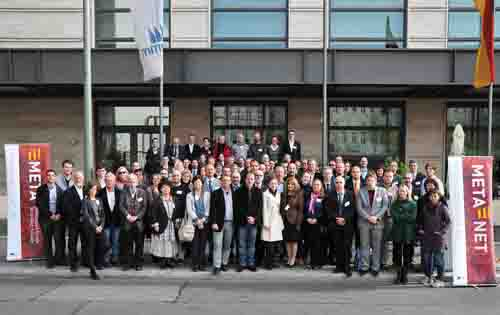
\includegraphics[width=\textwidth]{../_media/meta-net_team.jpg}
  \caption{Hizkuntza-teknologietako 100 bat adituk --META-NETen aurkezten diren herrialde eta hizkuntzetako ordezkariak-- Liburu Zurien bildumaren ondorio eta mezurik garrantzitsuenak aztertu eta finkatu zituzten, Berlinen, Alemanian, izandako bilera batean, 2011ko urriaren 21 eta 22an. ---
 \textcolor{grey1}{About 100 language technology experts -- representatives of the countries and languages represented in META-NET -- discussed and finalised the key results and messages of the White Paper Series at a META-NET meeting in Berlin, Germany, on October 21/22, 2011.}}
  \medskip
  \colorrule{grey3}{\textwidth}{1.5pt}
\end{figure*}

\cleardoublepage

\phantomsection\bsection[META-NETen liburu zurien bilduma -- The META-NET White Paper Series]{META-NETen liburu zurien bilduma --- The META-NET\ \ \ \ \ \ White Paper Series}
\label{whitepaperseries}

\vspace*{-5mm}
\centering
  \setlength{\tabcolsep}{2em}
  \begin{tabularx}{\textwidth}{lllll} \toprule\addlinespace
  %\begin{tabulary}{170mm}{LLL} \toprule
  Alemana & German & Deutsch\\
  Bulgariera & Bulgarian & български \\
  Daniera & Danish & dansk\\
  Errumaniera & Romanian & română\\  
  Eslovakiera & Slovak & slovenčina\\
  Esloveniera & Slovene & slovenščina\\
  Espainiera & Spanish & español\\
  Estoniera & Estonian & eesti\\
  Euskara & Basque & euskara\\
  Finlandiera & Finnish & suomi\\
  Frantsesa & French & français\\
  Galiziera & Galician & galego\\
  Grekera & Greek & ελληνικά\\
  Hungariera & Hungarian & magyar\\ 
  Ingelesa & English & English\\
  Irlandera & Irish & Gaeilge\\
  Islandiera & Icelandic & íslenska\\
  Italiera & Italian & italiano\\
  Katalana & Catalan & català\\
  Kroaziera & Croatian & hrvatski\\
  Letoniera & Latvian & latviešu valoda\\
  Lituaniera & Lithuanian & lietuvių kalba\\
  Maltera & Maltese & Malti\\
  Nederlandera & Dutch & Nederlands\\ 
  Norvegiera Bokmål & Norwegian Bokmål & bokmål\\
  Norvegiera Nynorsk & Norwegian Nynorsk & nynorsk\\
  Poloniera & Polish & polski\\
  Portugalera & Portuguese & português\\
  Serbiera & Serbian & српски\\
  Suediera & Swedish & svenska\\
  Txekiera & Czech & čeština\\  \addlinespace \bottomrule
\end{tabularx}
